\documentclass[12pt]{extarticle}
\usepackage[paperwidth=18in,paperheight=7.5in]{geometry}
\usepackage{amsmath}
\usepackage{hyperref}
\usepackage{multirow}
\usepackage{pdfpages}
\usepackage[utf8]{inputenc}
\title{Kaon mixing: chiral and continuum extrapolations}
\author{R Mukherjee}
\date{\today}
\begin{document}
\maketitle
\tableofcontents
\clearpage
\begin{figure}
\centering
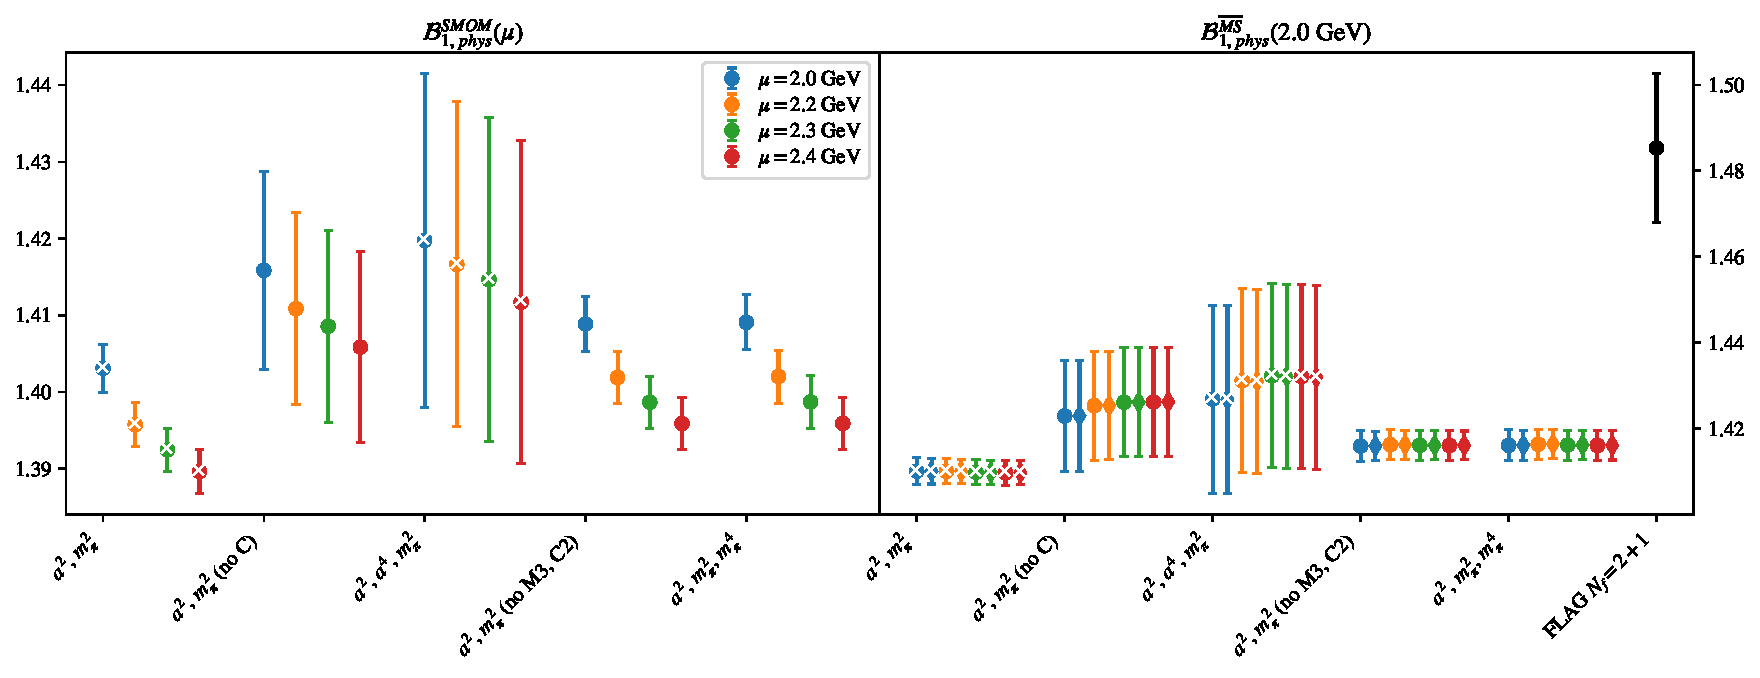
\includegraphics[page=1, width=1.1\textwidth]{VVpAA/SUSY/fit_summary_bag.pdf}
\caption{$\mathcal{B}_{1}$\\(left) $\mathcal{B}_{phys}$ in RI/SMOM scheme from fit variations (fits with $p$-value $<0.05$ marked with ``$\times$"). \\(right) $\mathcal{B}_{phys}$ in $\overline{MS}$ computed using $\mathcal{B}^{\overline{MS}} = R^{\overline{MS}\leftarrow SMOM}(2.0)\sigma_{npt}(2.0,\mu) \mathcal{B}^{SMOM}(\mu)$.}
\end{figure}
\clearpage
\begin{figure}
\centering
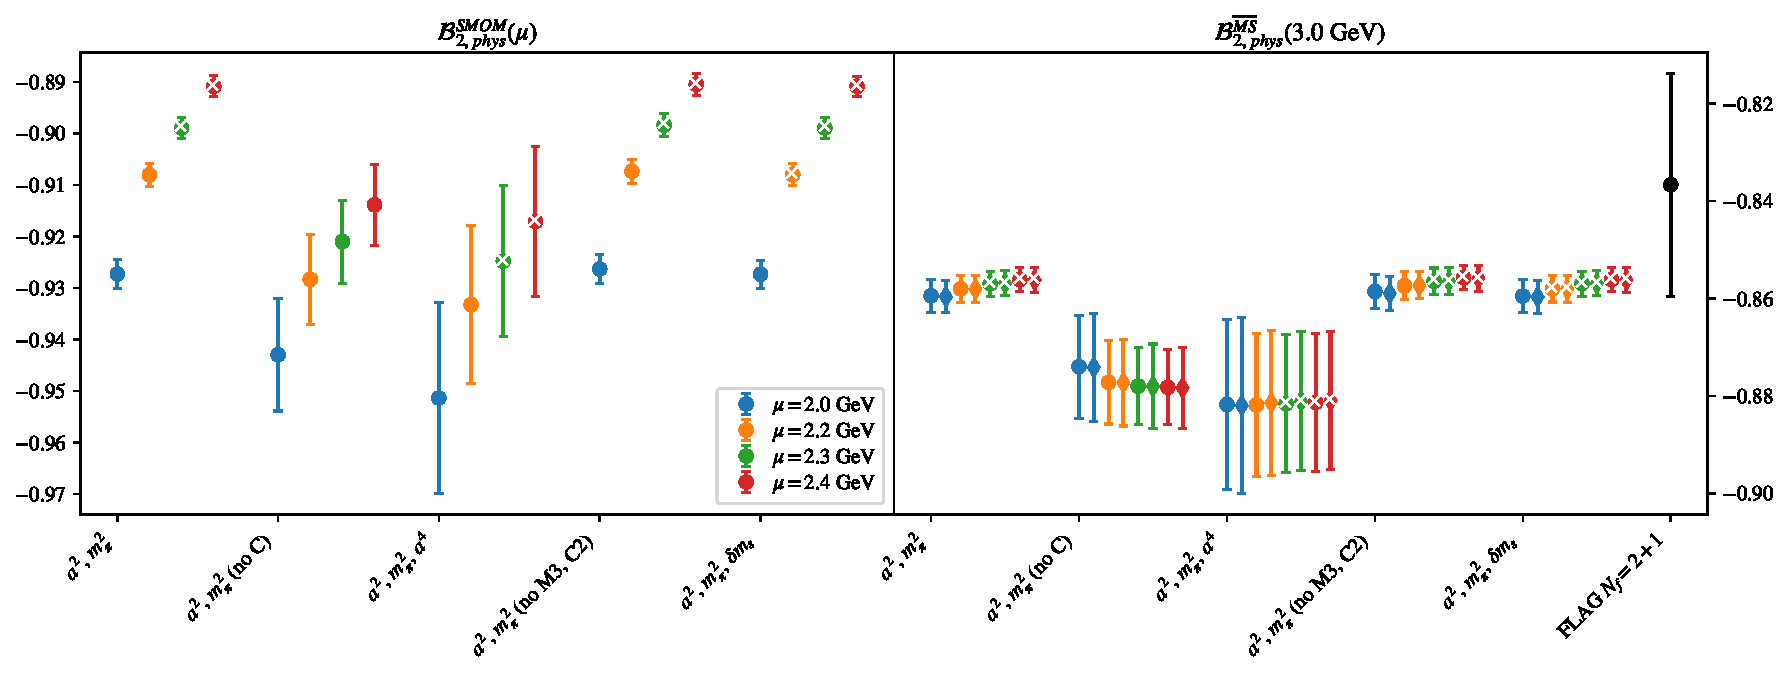
\includegraphics[page=1, width=1.1\textwidth]{VVmAA/SUSY/fit_summary_bag.pdf}
\caption{$\mathcal{B}_{2}$\\(left) $\mathcal{B}_{phys}$ in RI/SMOM scheme from fit variations (fits with $p$-value $<0.05$ marked with ``$\times$"). \\(right) $\mathcal{B}_{phys}$ in $\overline{MS}$ computed using $\mathcal{B}^{\overline{MS}} = R^{\overline{MS}\leftarrow SMOM}(3.0)\sigma_{npt}(3.0,\mu) \mathcal{B}^{SMOM}(\mu)$.}
\end{figure}
\clearpage
\begin{figure}
\centering
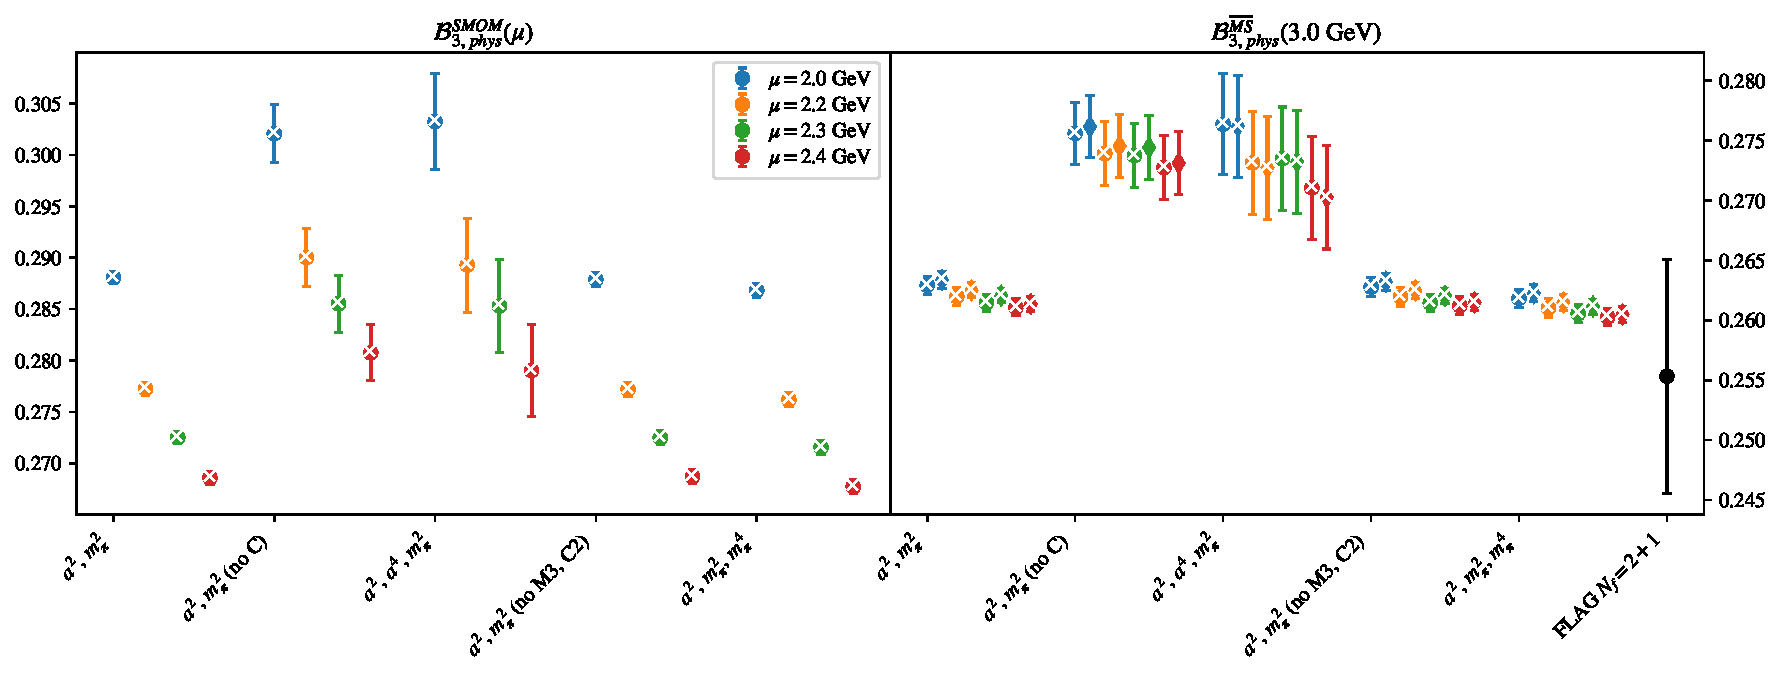
\includegraphics[page=1, width=1.1\textwidth]{SSmPP/SUSY/fit_summary_bag.pdf}
\caption{$\mathcal{B}_{3}$\\(left) $\mathcal{B}_{phys}$ in RI/SMOM scheme from fit variations (fits with $p$-value $<0.05$ marked with ``$\times$"). \\(right) $\mathcal{B}_{phys}$ in $\overline{MS}$ computed using $\mathcal{B}^{\overline{MS}} = R^{\overline{MS}\leftarrow SMOM}(3.0)\sigma_{npt}(3.0,\mu) \mathcal{B}^{SMOM}(\mu)$.}
\end{figure}
\clearpage
\begin{figure}
\centering
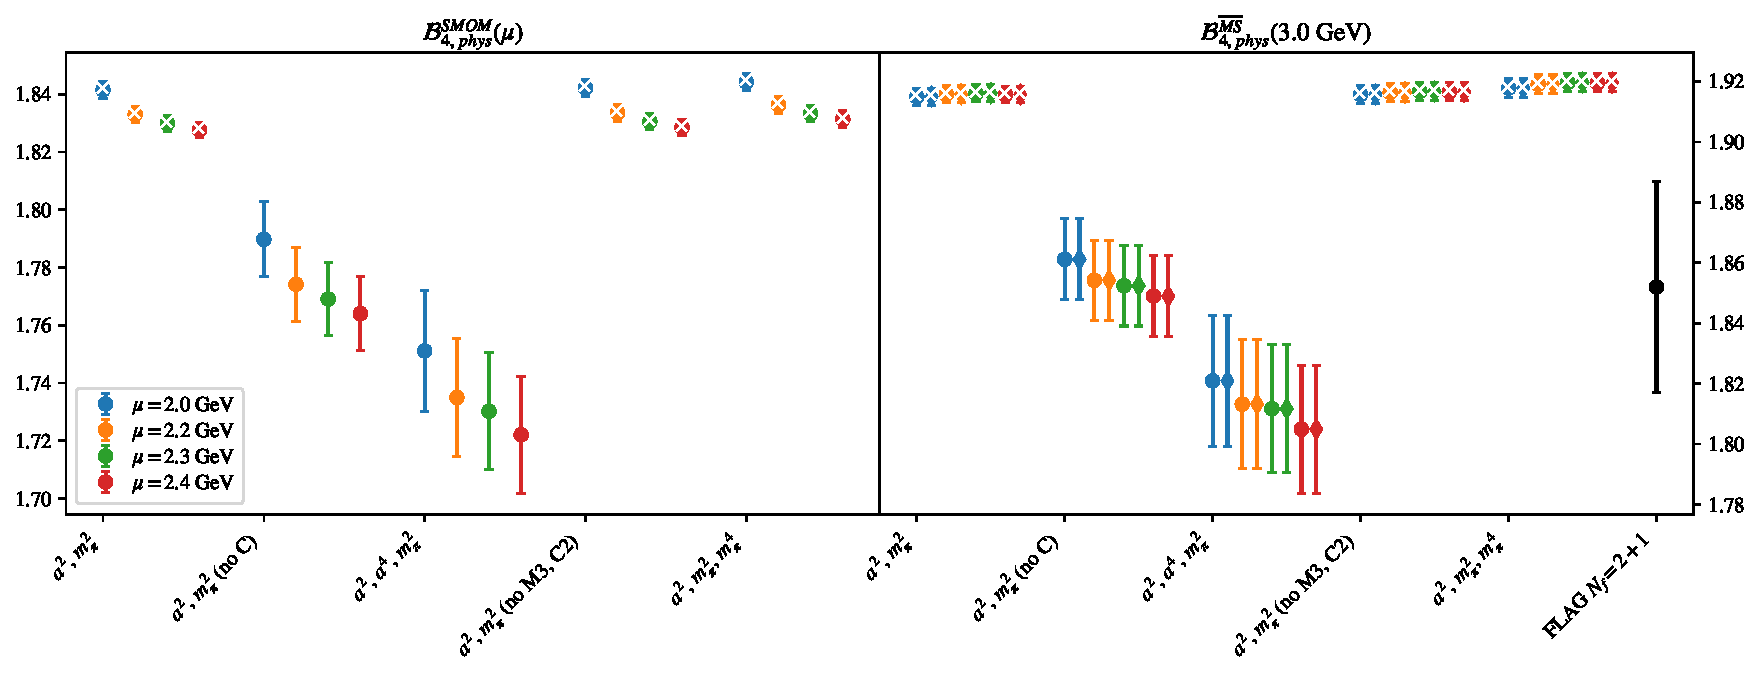
\includegraphics[page=1, width=1.1\textwidth]{SSpPP/SUSY/fit_summary_bag.pdf}
\caption{$\mathcal{B}_{4}$\\(left) $\mathcal{B}_{phys}$ in RI/SMOM scheme from fit variations (fits with $p$-value $<0.05$ marked with ``$\times$"). \\(right) $\mathcal{B}_{phys}$ in $\overline{MS}$ computed using $\mathcal{B}^{\overline{MS}} = R^{\overline{MS}\leftarrow SMOM}(3.0)\sigma_{npt}(3.0,\mu) \mathcal{B}^{SMOM}(\mu)$.}
\end{figure}
\clearpage
\begin{figure}
\centering
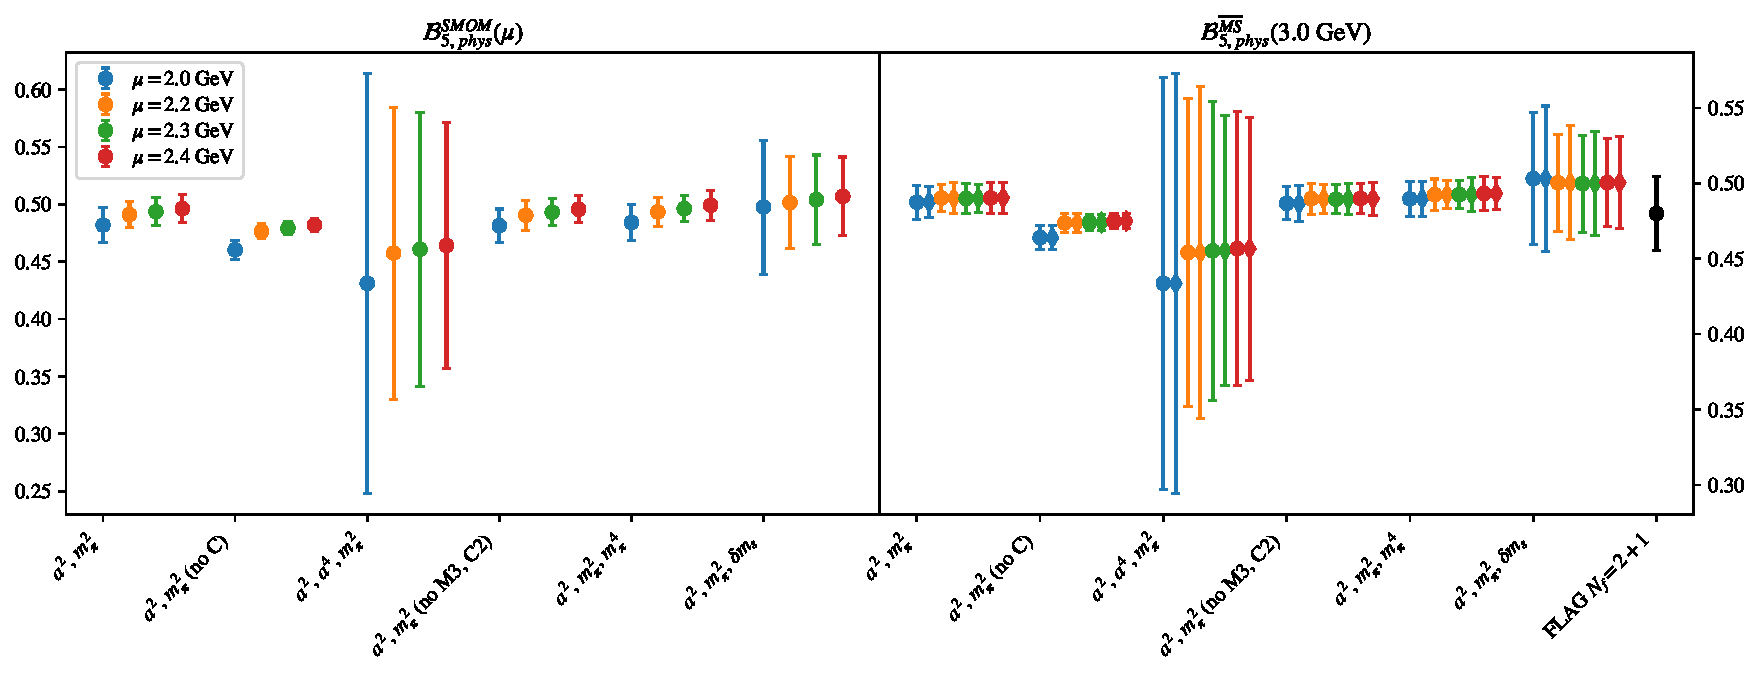
\includegraphics[page=1, width=1.1\textwidth]{TT/SUSY/fit_summary_bag.pdf}
\caption{$\mathcal{B}_{5}$\\(left) $\mathcal{B}_{phys}$ in RI/SMOM scheme from fit variations (fits with $p$-value $<0.05$ marked with ``$\times$"). \\(right) $\mathcal{B}_{phys}$ in $\overline{MS}$ computed using $\mathcal{B}^{\overline{MS}} = R^{\overline{MS}\leftarrow SMOM}(3.0)\sigma_{npt}(3.0,\mu) \mathcal{B}^{SMOM}(\mu)$.}
\end{figure}
\clearpage
\section{$\mathcal{B}_1$}
\begin{table}[h!]
\begin{center}
\begin{tabular}{|c|c|c|c|c|c|c|}
\hline
$\mu$ (GeV) & $a^2$, $m_\pi^2$& $a^2$, $m_\pi^2$ (no C)& $a^2$, $a^4$, $m_\pi^2$& $a^2$, $m_\pi^2$ (no M3, C2)& $a^2$, $m_\pi^2$, $m_\pi^4$& $a^2$, $m_\pi^2$, $\delta m_s$\\
\hline
2.0& \hyperlink{VVpAA/SUSY/a2m2_20.pdf.1}{\textbf{1.4024(27)}: 2.268 (0.045)} & \hyperlink{VVpAA/SUSY/a2m2noC_20.pdf.1}{\textbf{1.415(12)}: 0.844 (0.43)} & \hyperlink{VVpAA/SUSY/a2a4m2_20.pdf.1}{\textbf{1.415(21)}: 2.744 (0.027)} & \hyperlink{VVpAA/SUSY/a2m2mcut_20.pdf.1}{\textbf{1.4080(32)}: 0.217 (0.885)} & \hyperlink{VVpAA/SUSY/a2m2m4_20.pdf.1}{\textbf{1.4080(33)}: 0.963 (0.426)} & \hyperlink{VVpAA/SUSY/a2m2delm_20.pdf.1}{\textbf{1.4000(34)}: 2.378 (0.05)}\\
2.2& \hyperlink{VVpAA/SUSY/a2m2_22.pdf.1}{\textbf{1.3950(27)}: 2.615 (0.023)} & \hyperlink{VVpAA/SUSY/a2m2noC_22.pdf.1}{\textbf{1.410(12)}: 0.984 (0.374)} & \hyperlink{VVpAA/SUSY/a2a4m2_22.pdf.1}{\textbf{1.412(21)}: 3.101 (0.015)} & \hyperlink{VVpAA/SUSY/a2m2mcut_22.pdf.1}{\textbf{1.4011(32)}: 0.356 (0.785)} & \hyperlink{VVpAA/SUSY/a2m2m4_22.pdf.1}{\textbf{1.4009(33)}: 1.215 (0.302)} & \hyperlink{VVpAA/SUSY/a2m2delm_22.pdf.1}{\textbf{1.3922(33)}: 2.606 (0.034)}\\
2.3& \hyperlink{VVpAA/SUSY/a2m2_23.pdf.1}{\textbf{1.3916(27)}: 2.839 (0.014)} & \hyperlink{VVpAA/SUSY/a2m2noC_23.pdf.1}{\textbf{1.408(12)}: 1.059 (0.347)} & \hyperlink{VVpAA/SUSY/a2a4m2_23.pdf.1}{\textbf{1.410(21)}: 3.339 (0.01)} & \hyperlink{VVpAA/SUSY/a2m2mcut_23.pdf.1}{\textbf{1.3979(32)}: 0.447 (0.719)} & \hyperlink{VVpAA/SUSY/a2m2m4_23.pdf.1}{\textbf{1.3977(33)}: 1.393 (0.234)} & \hyperlink{VVpAA/SUSY/a2m2delm_23.pdf.1}{\textbf{1.3885(33)}: 2.759 (0.026)}\\
2.4& \hyperlink{VVpAA/SUSY/a2m2_24.pdf.1}{\textbf{1.3887(27)}: 2.946 (0.012)} & \hyperlink{VVpAA/SUSY/a2m2noC_24.pdf.1}{\textbf{1.406(12)}: 1.112 (0.329)} & \hyperlink{VVpAA/SUSY/a2a4m2_24.pdf.1}{\textbf{1.408(21)}: 3.462 (0.008)} & \hyperlink{VVpAA/SUSY/a2m2mcut_24.pdf.1}{\textbf{1.3951(32)}: 0.469 (0.704)} & \hyperlink{VVpAA/SUSY/a2m2m4_24.pdf.1}{\textbf{1.3949(32)}: 1.449 (0.215)} & \hyperlink{VVpAA/SUSY/a2m2delm_24.pdf.1}{\textbf{1.3856(33)}: 2.846 (0.023)}\\
\hline
\end{tabular}
\caption{Physical point value from chiral and continuum extrapolation at renormalisation scale $\mu$. Entries are \textbf{value(error)}: $\chi^2/\text{DOF}$ ($p$-value).}
\end{center}
\end{table}
\begin{table}[h!]
\begin{center}
\begin{tabular}{|c c|c|c|c|c|c|c|}
\hline
$\mu$ (GeV) &  & $a^2$, $m_\pi^2$& $a^2$, $m_\pi^2$ (no C)& $a^2$, $a^4$, $m_\pi^2$& $a^2$, $m_\pi^2$ (no M3, C2)& $a^2$, $m_\pi^2$, $m_\pi^4$& $a^2$, $m_\pi^2$, $\delta m_s$\\
\hline
\multirow{2}{0.5in}{2.0} & $\alpha$ & 0.0975(73)& 0.052(53)& 0.014& 0.0838(83)& 0.0844(83)& 0.1030(87)\\
 & $\beta$ & 0.00288(16)& 0.00231(32)& 0.00289(16)& 0.00206(32)& 0.00034(95)& 0.00296(17)\\
\hline
\multirow{2}{0.5in}{2.2} & $\alpha$ & 0.1014(73)& 0.044(53)& -0.012& 0.0868(83)& 0.0877(83)& 0.1080(87)\\
 & $\beta$ & 0.00282(15)& 0.00222(31)& 0.00284(15)& 0.00196(31)& 0.00019(94)& 0.00291(16)\\
\hline
\multirow{2}{0.5in}{2.3} & $\alpha$ & 0.1033(73)& 0.039(53)& -0.023& 0.0880(83)& 0.0892(83)& 0.1104(86)\\
 & $\beta$ & 0.00280(15)& 0.00218(31)& 0.00283(15)& 0.00192(31)& 0.00011(94)& 0.00291(16)\\
\hline
\multirow{2}{0.5in}{2.4} & $\alpha$ & 0.1041(73)& 0.039(52)& -0.025& 0.0884(83)& 0.0896(83)& 0.1114(86)\\
 & $\beta$ & 0.00279(15)& 0.00216(30)& 0.00282(15)& 0.00190(31)& 0.0& 0.00290(16)\\
\hline
\end{tabular}
\caption{Fit values of coefficients in $Q = Q_{phys} + \mathbf{\alpha} a^2 + \mathbf{\beta}\left(\frac{m_\pi^2}{f_\pi^2}-\frac{m_{\pi,PDG}^2}{f_\pi^2}\right) + \ldots$.}
\end{center}
\end{table}
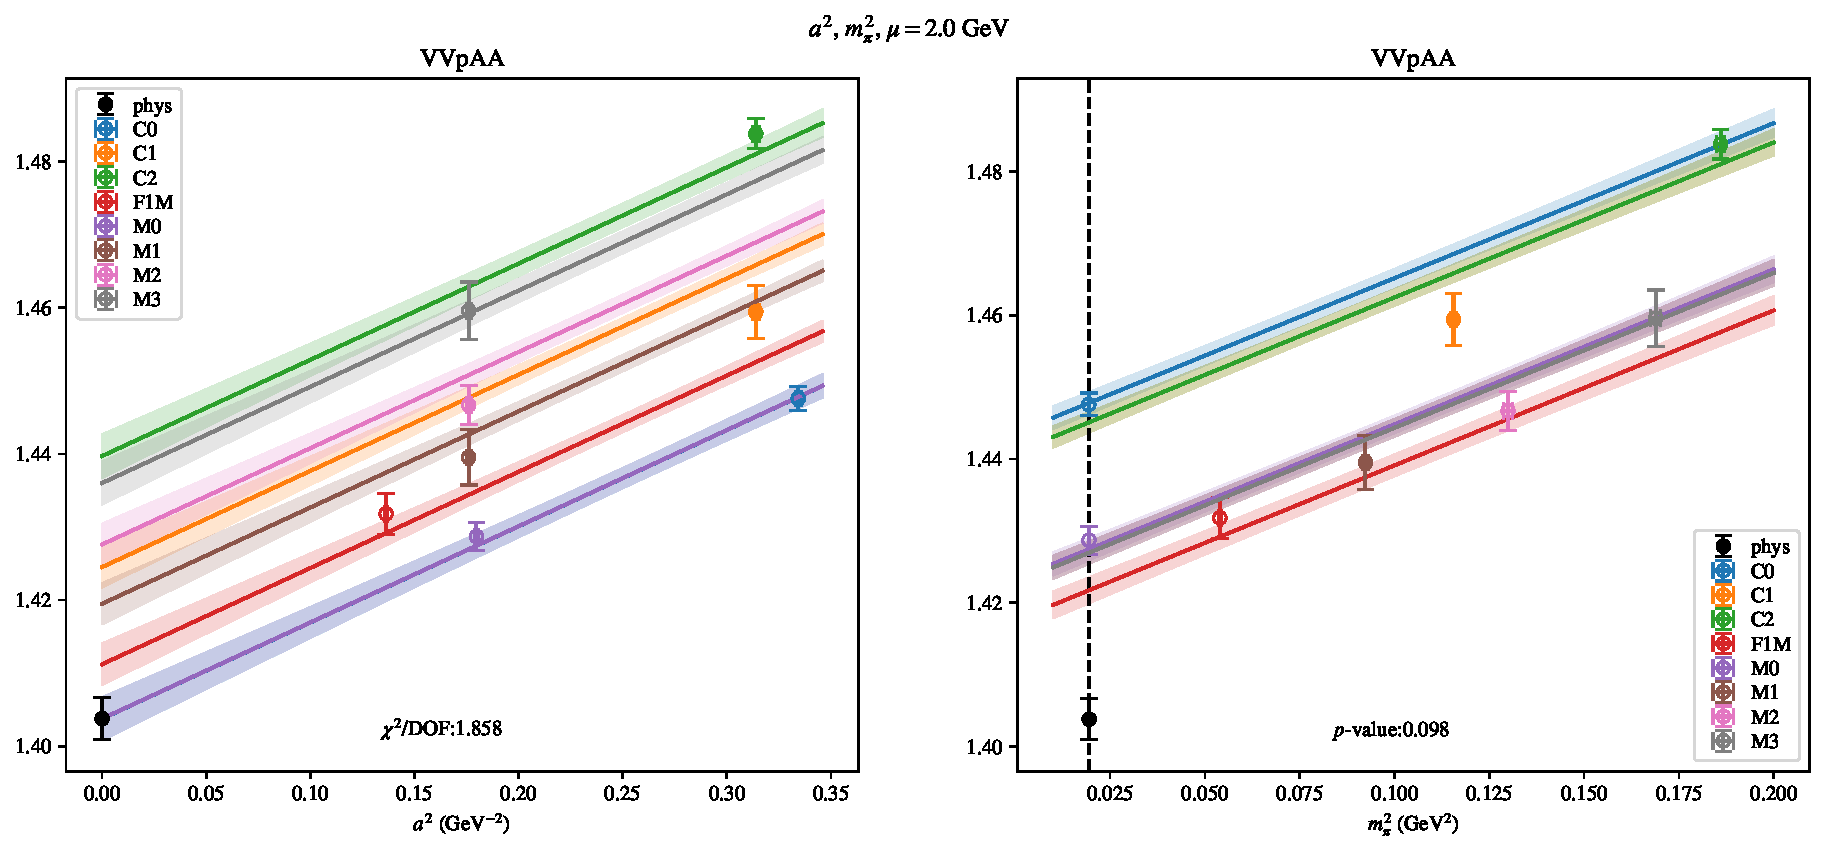
\includepdf[link, pages=-]{VVpAA/SUSY/a2m2_20.pdf}
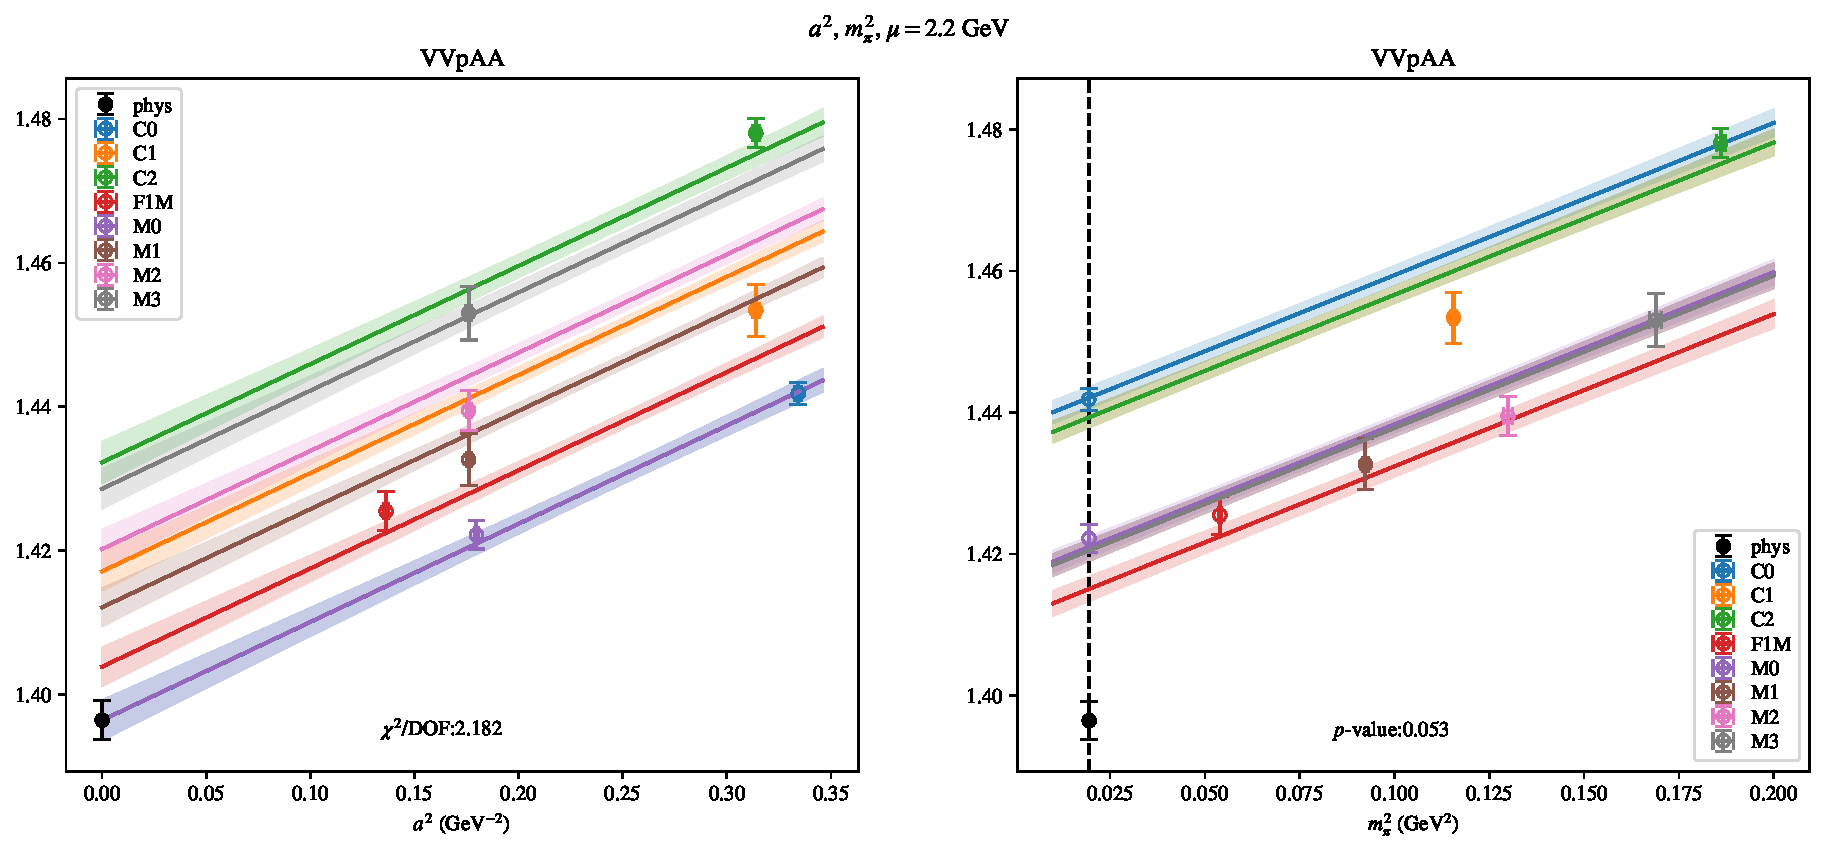
\includepdf[link, pages=-]{VVpAA/SUSY/a2m2_22.pdf}
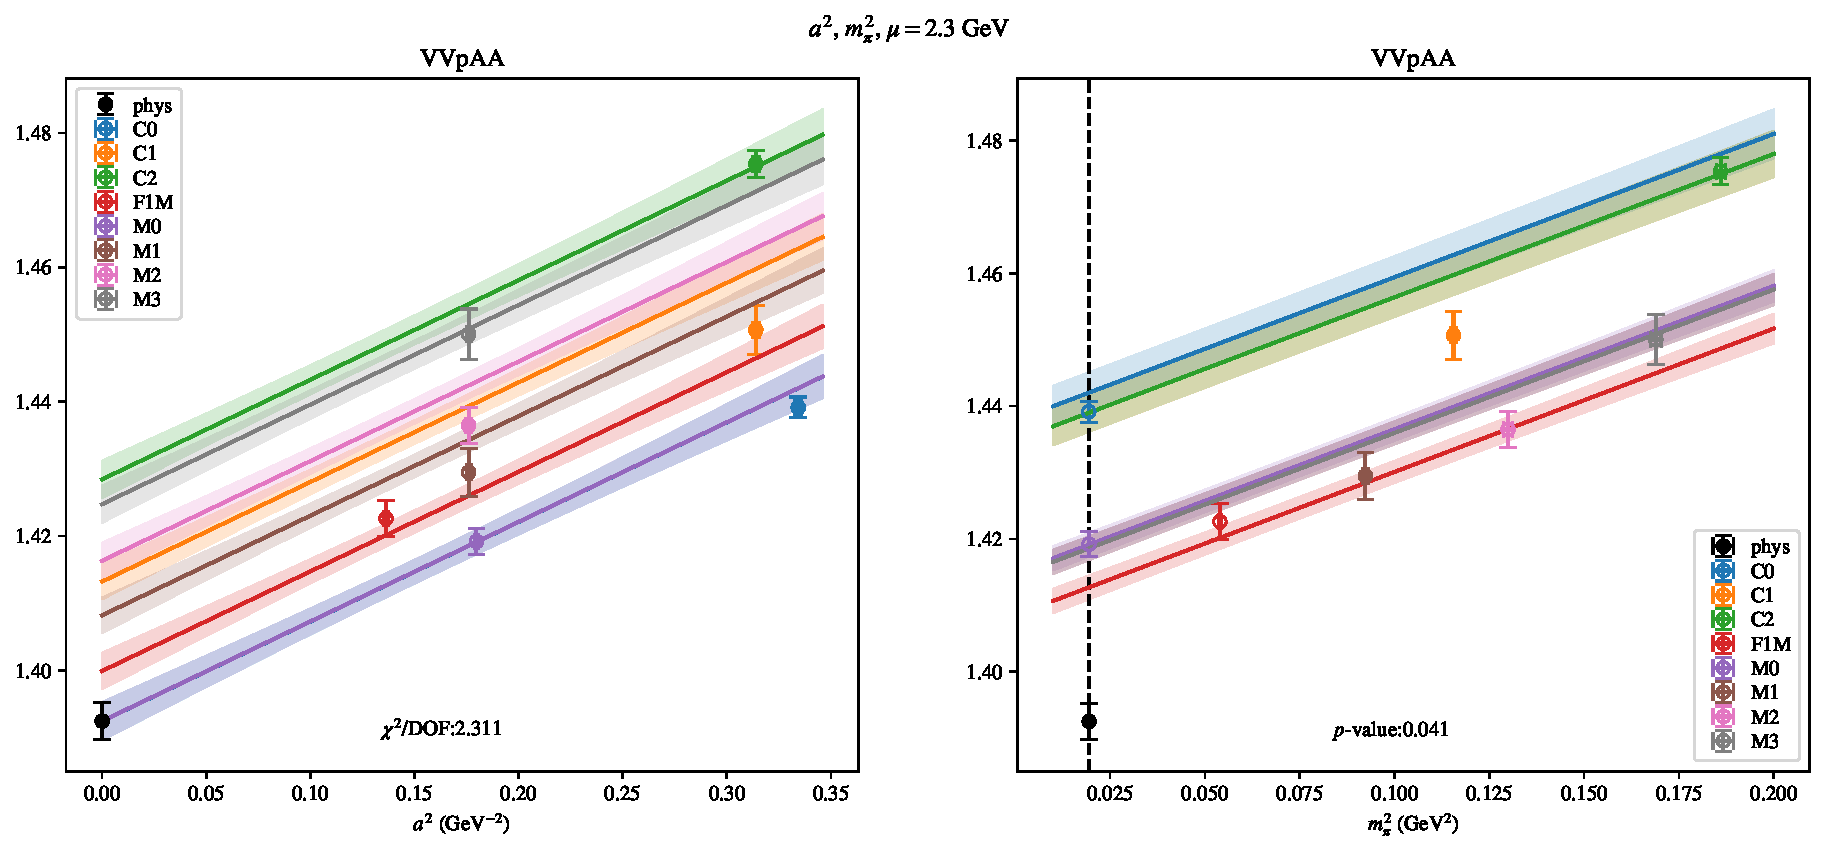
\includepdf[link, pages=-]{VVpAA/SUSY/a2m2_23.pdf}
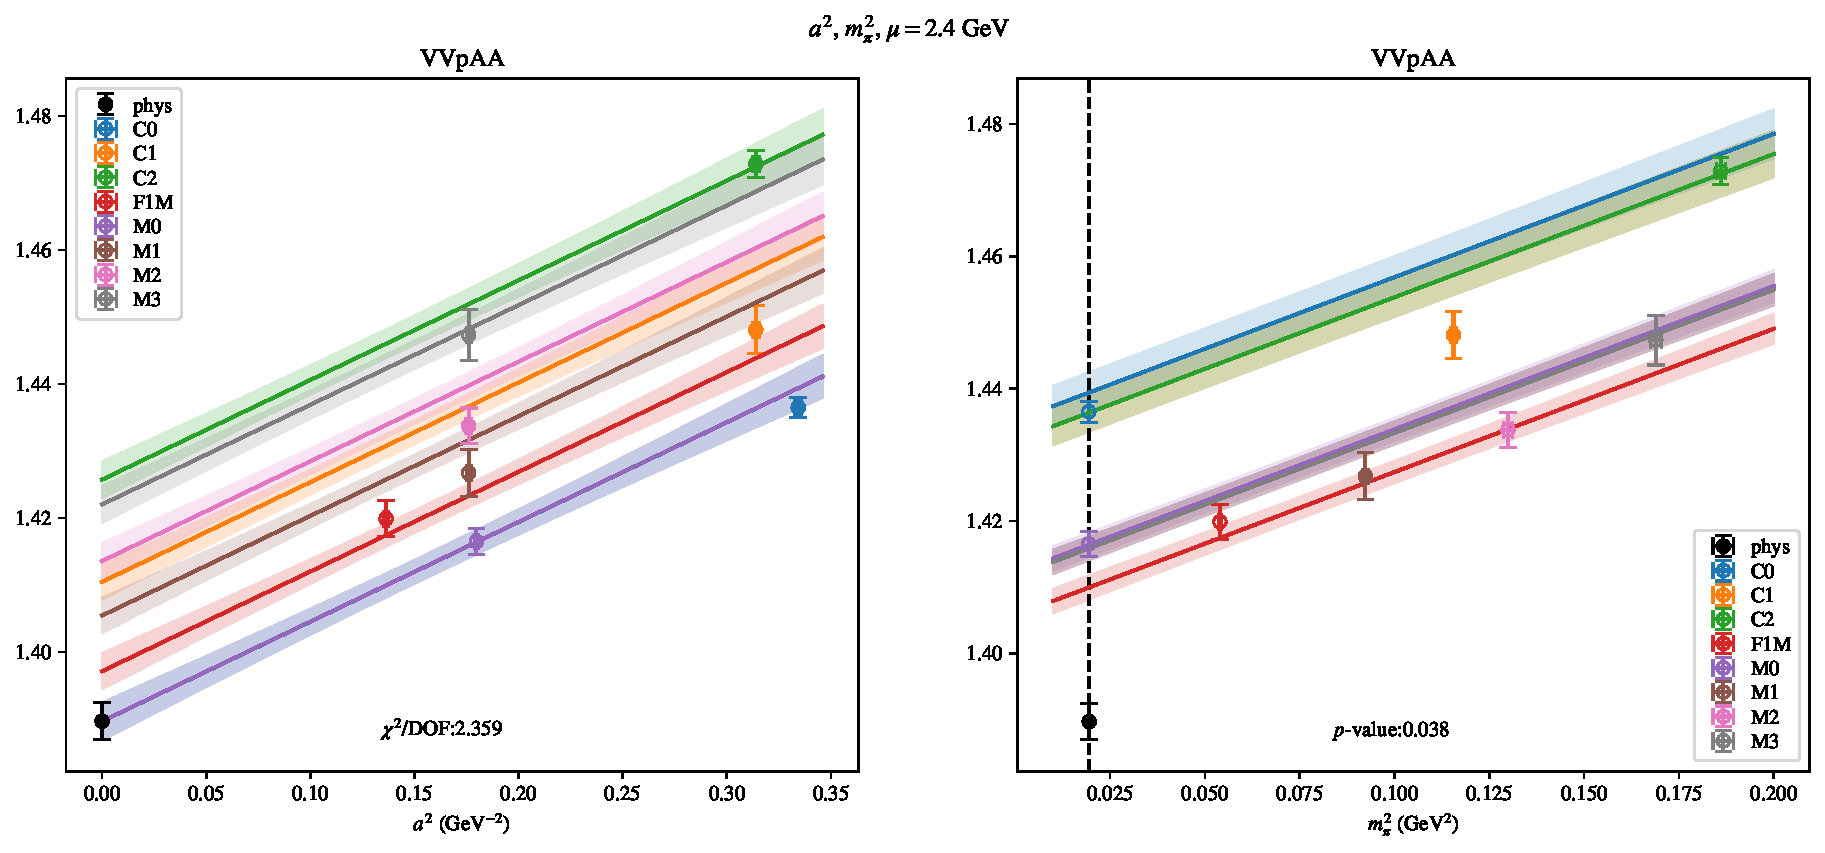
\includepdf[link, pages=-]{VVpAA/SUSY/a2m2_24.pdf}
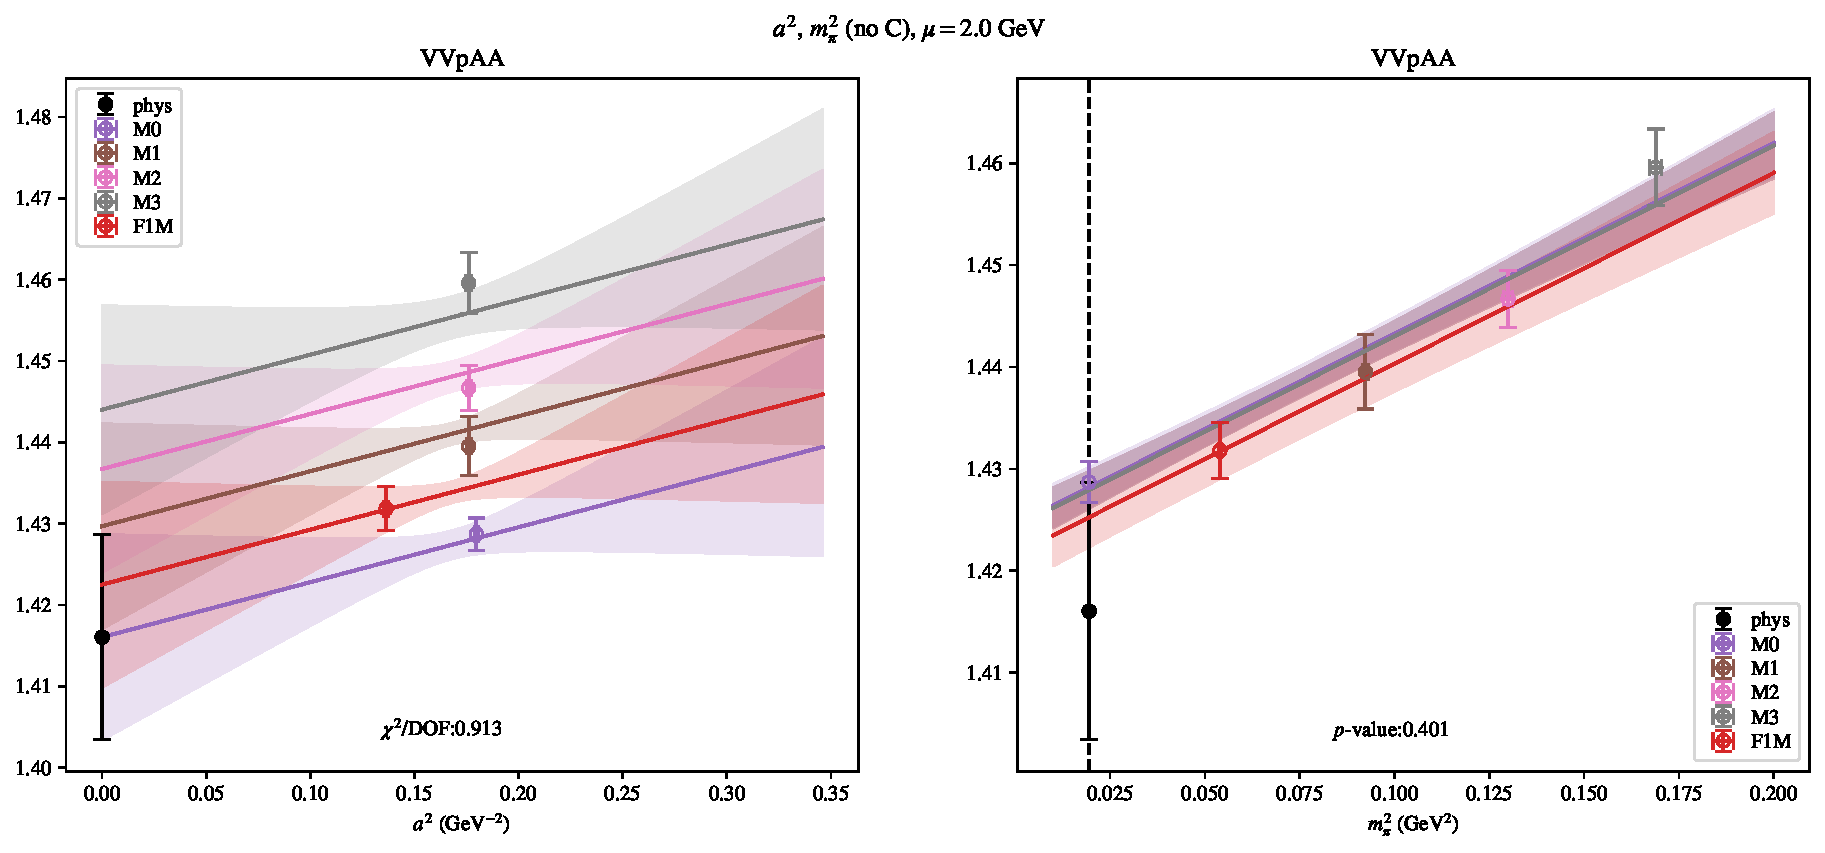
\includepdf[link, pages=-]{VVpAA/SUSY/a2m2noC_20.pdf}
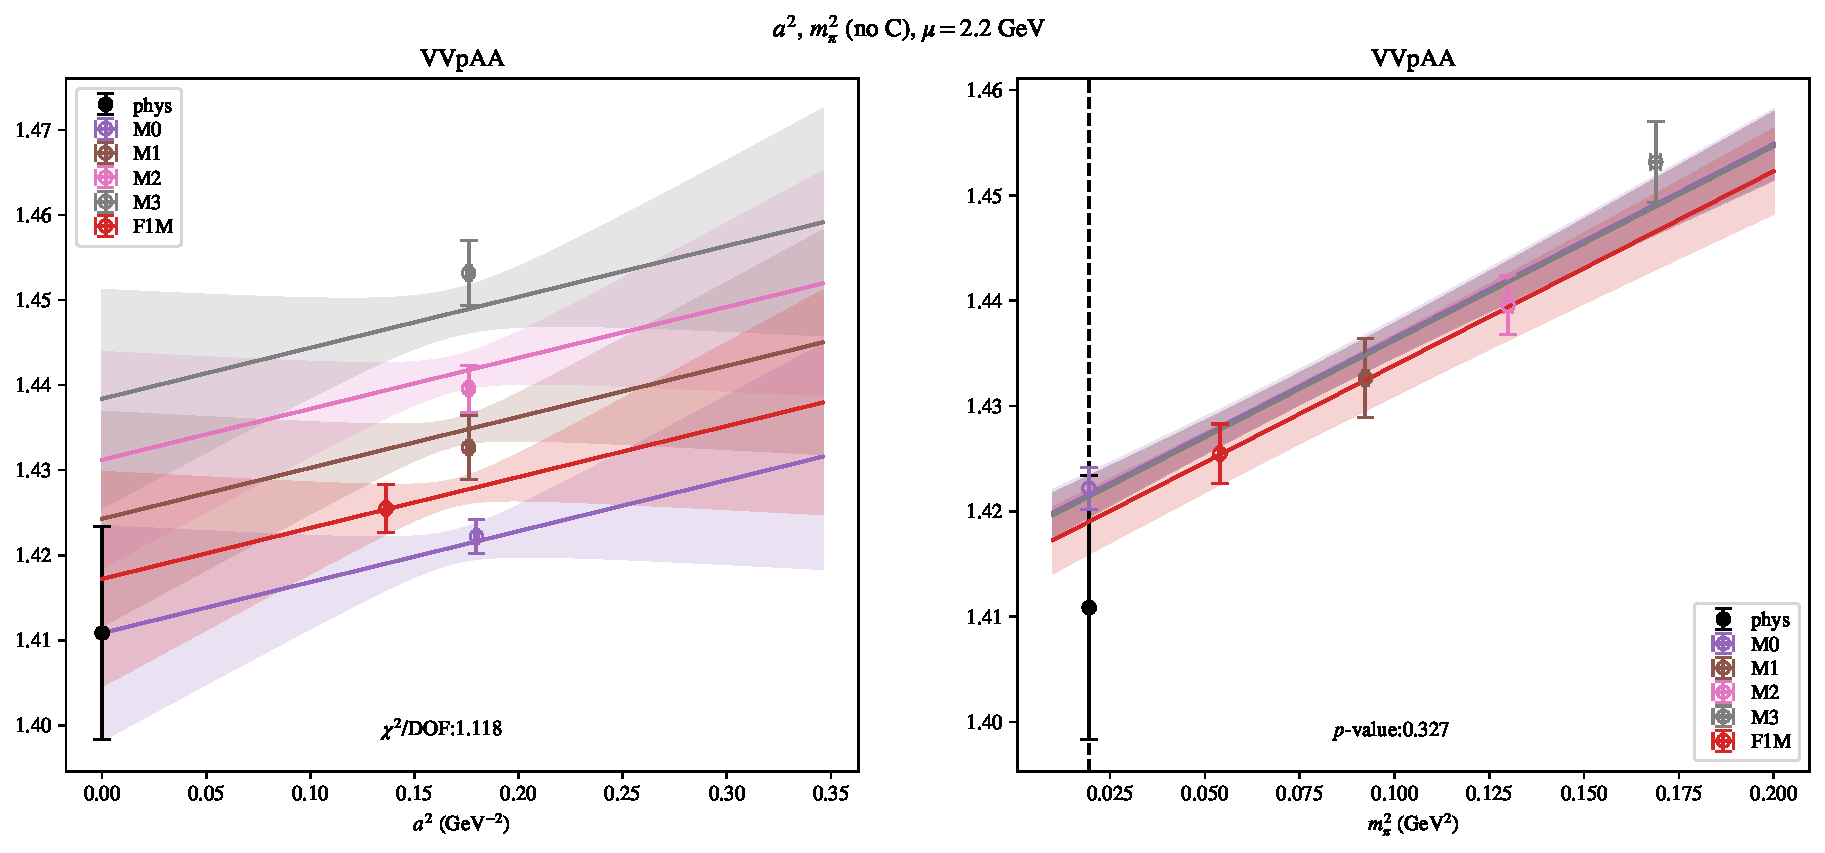
\includepdf[link, pages=-]{VVpAA/SUSY/a2m2noC_22.pdf}
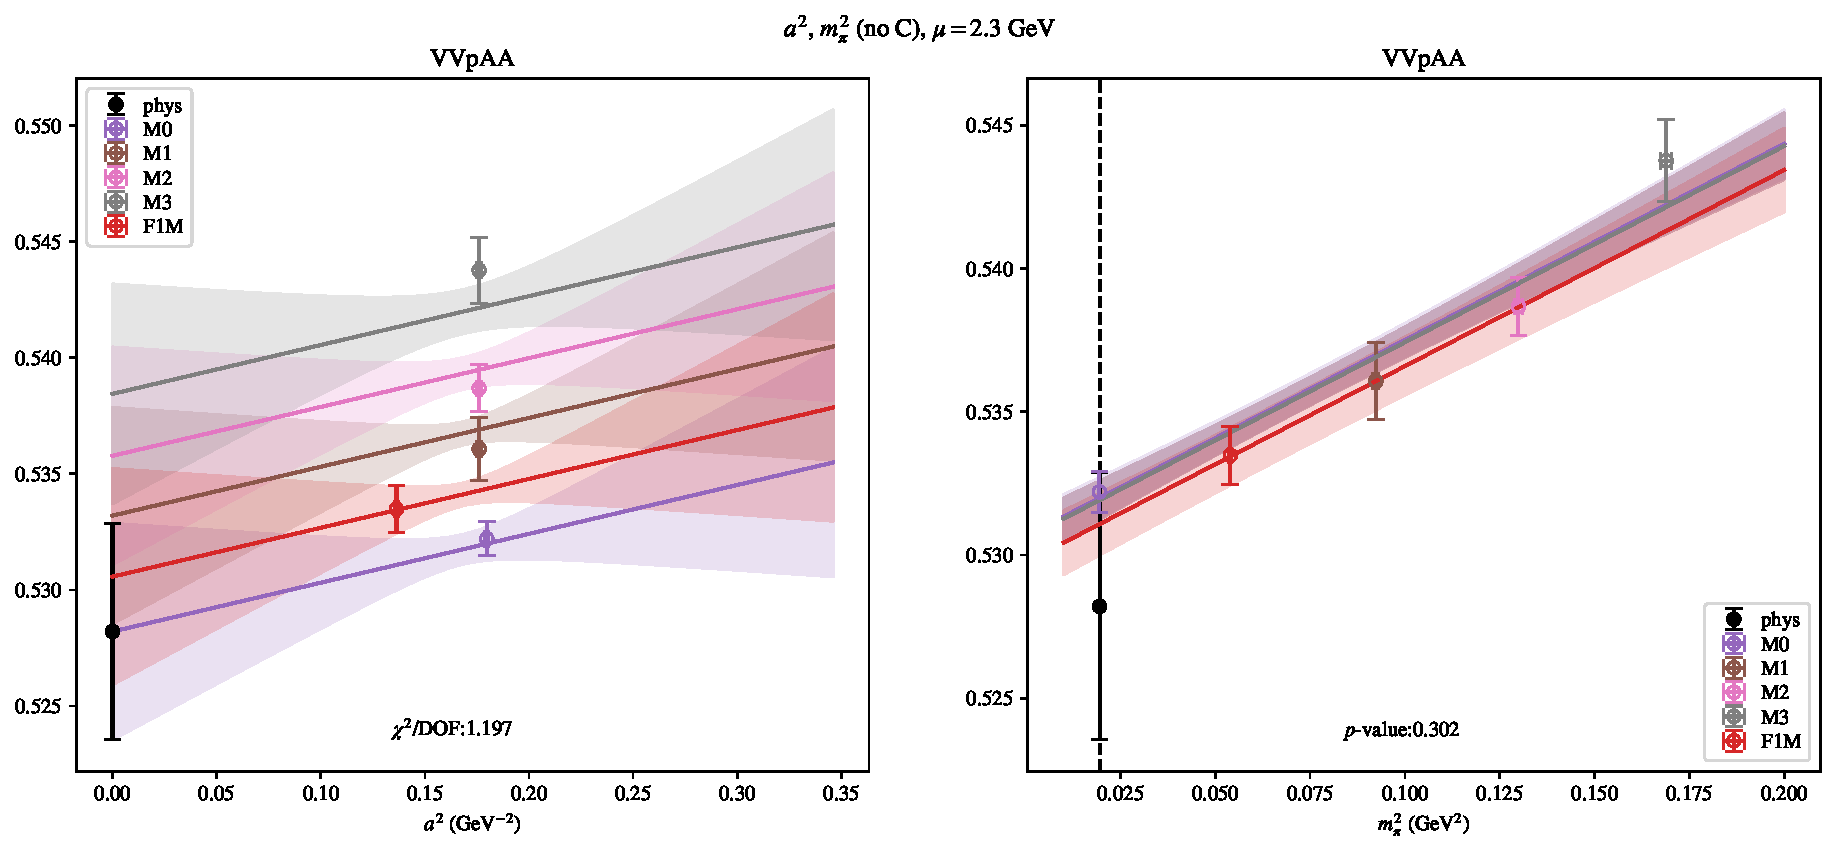
\includepdf[link, pages=-]{VVpAA/SUSY/a2m2noC_23.pdf}
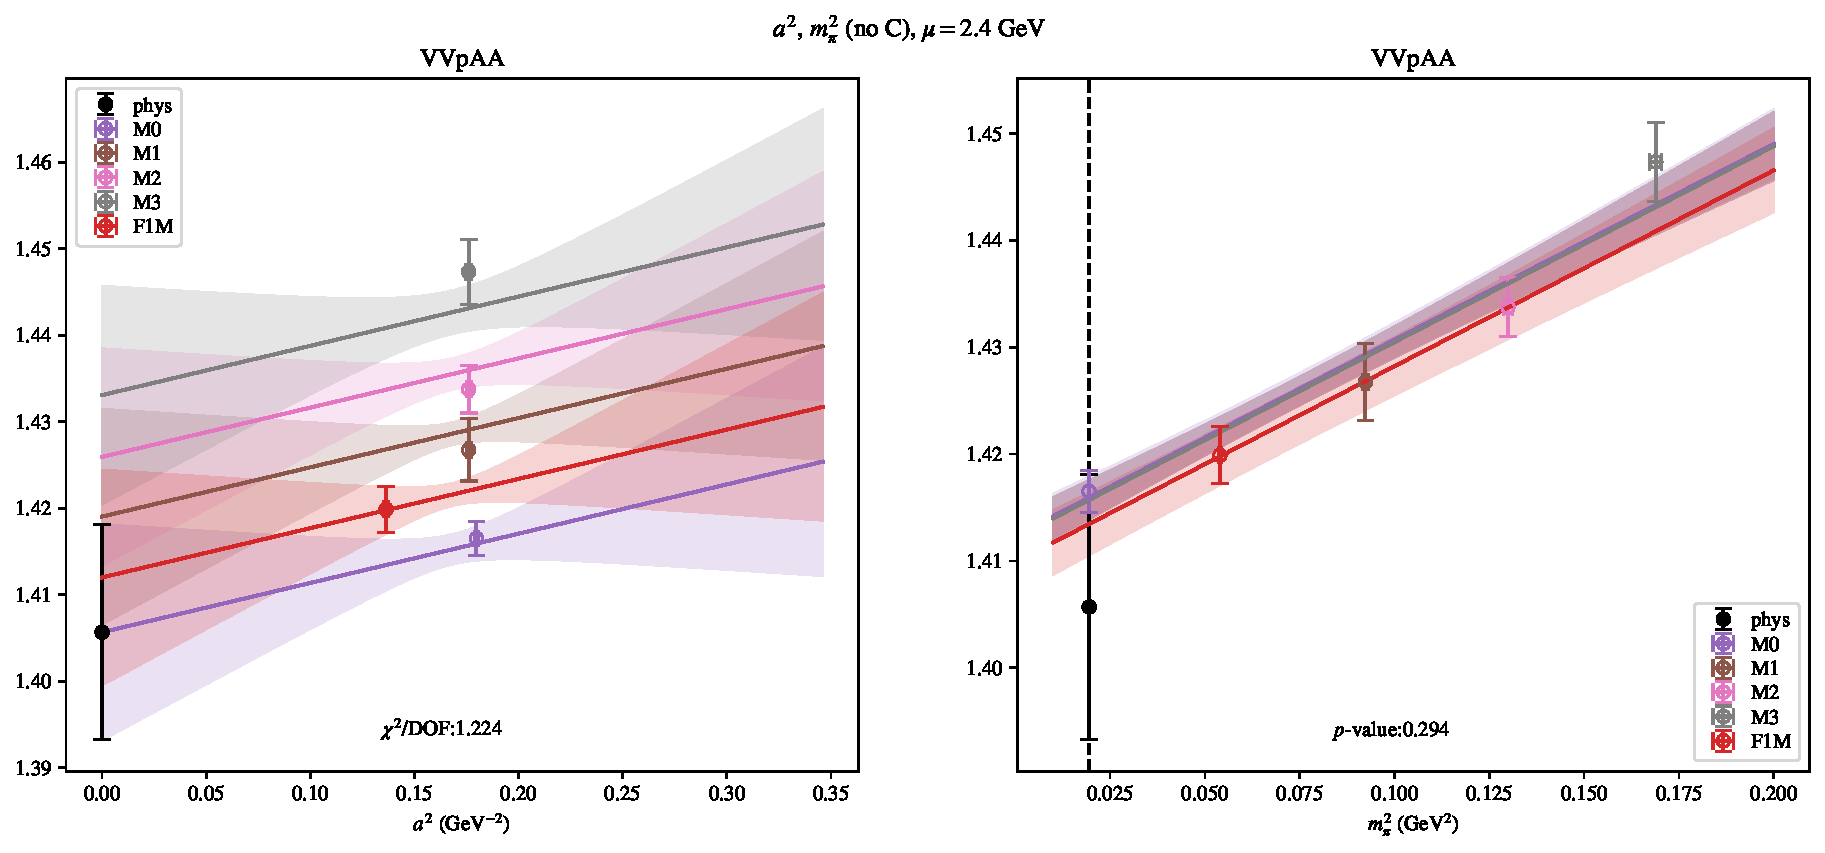
\includepdf[link, pages=-]{VVpAA/SUSY/a2m2noC_24.pdf}
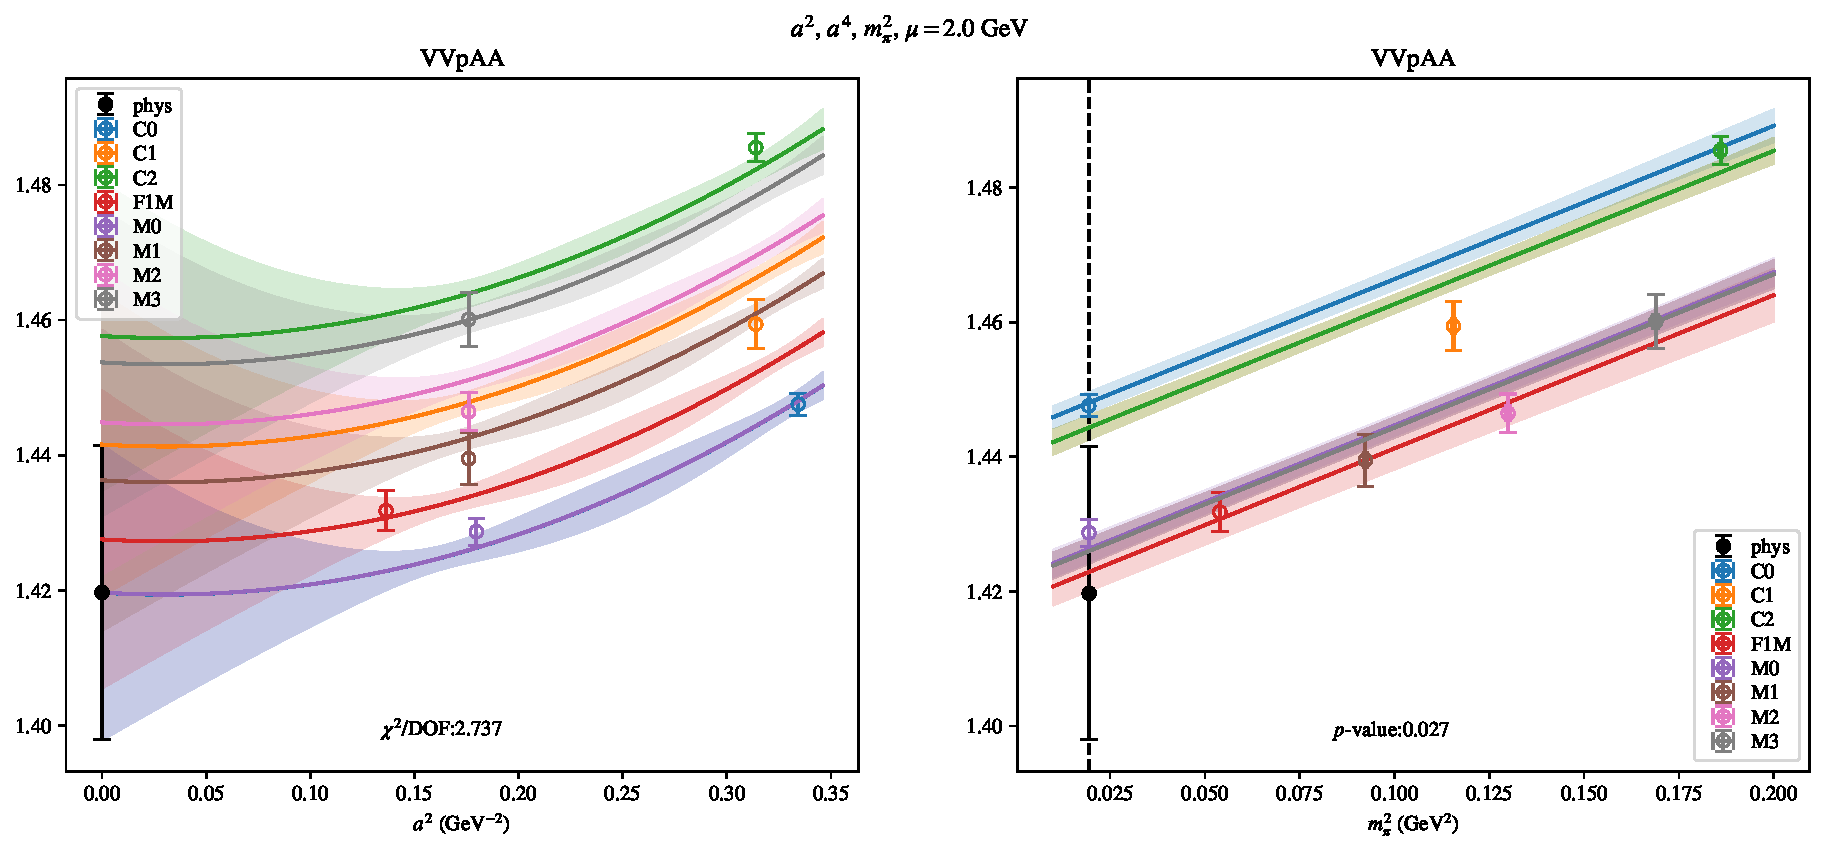
\includepdf[link, pages=-]{VVpAA/SUSY/a2a4m2_20.pdf}
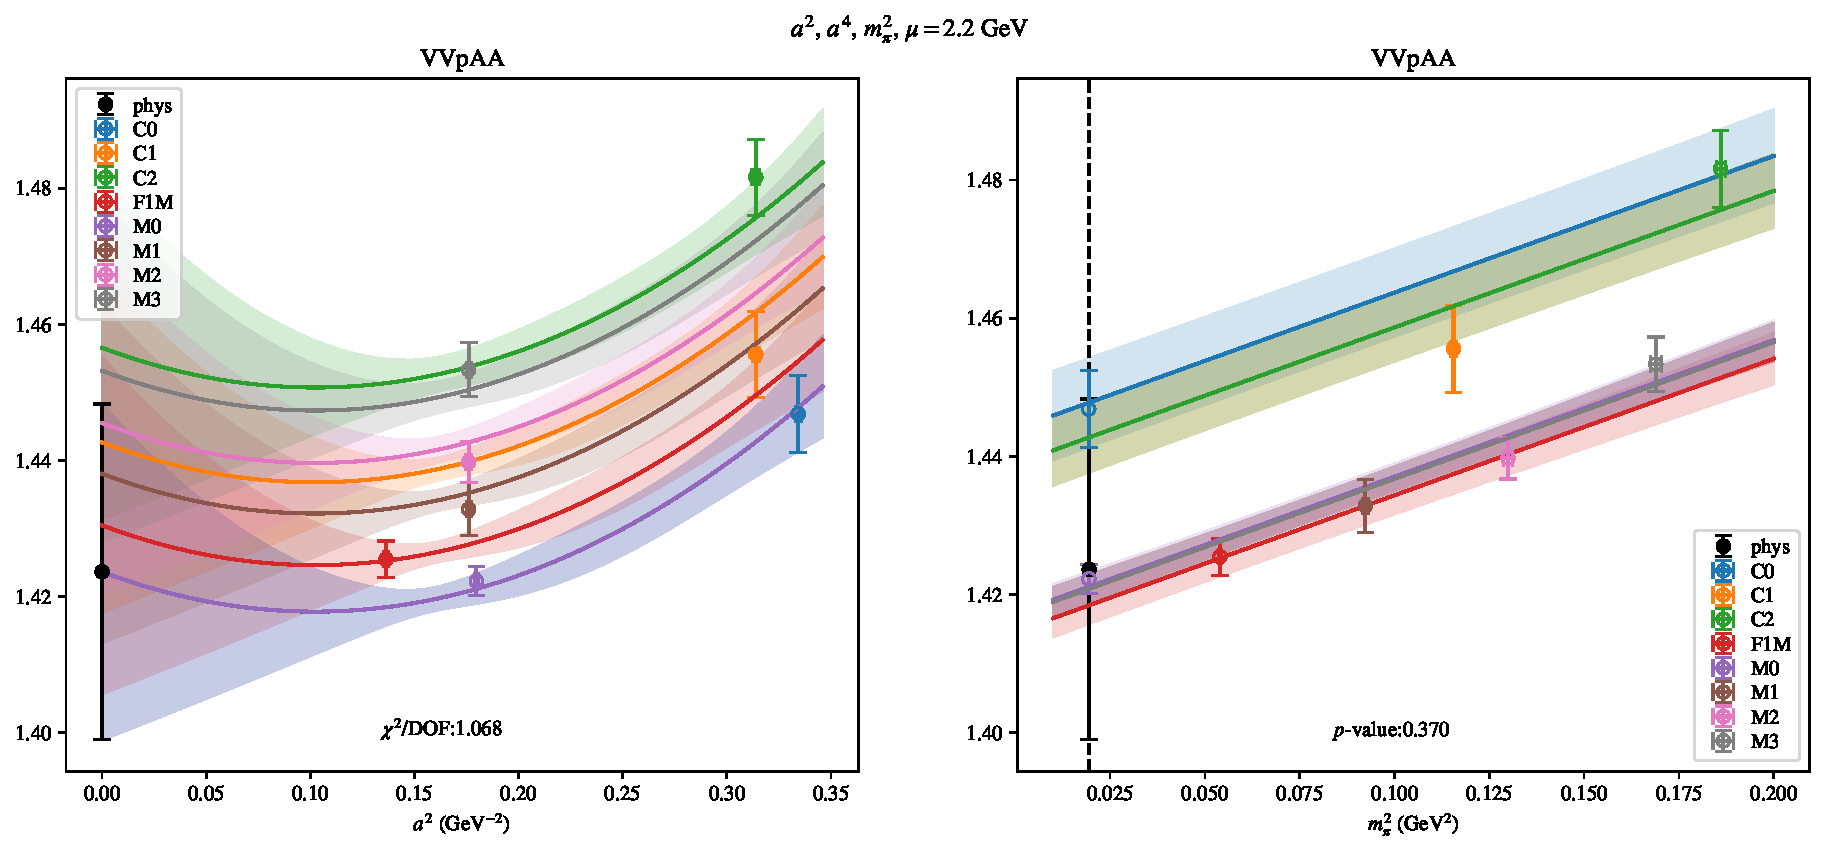
\includepdf[link, pages=-]{VVpAA/SUSY/a2a4m2_22.pdf}
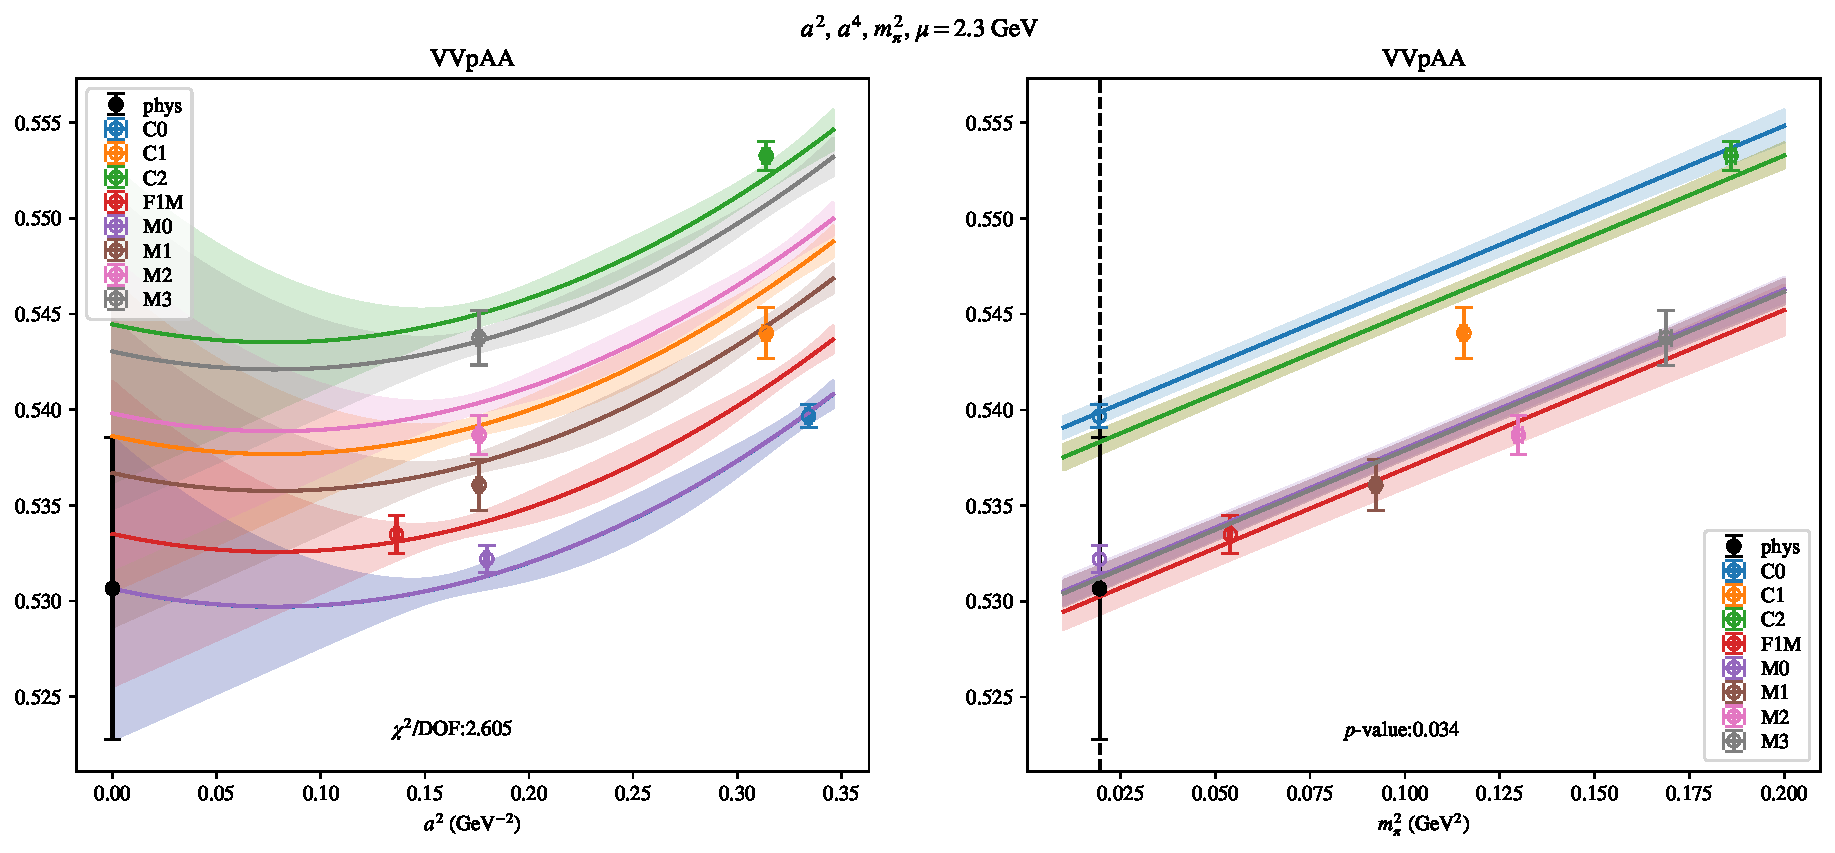
\includepdf[link, pages=-]{VVpAA/SUSY/a2a4m2_23.pdf}
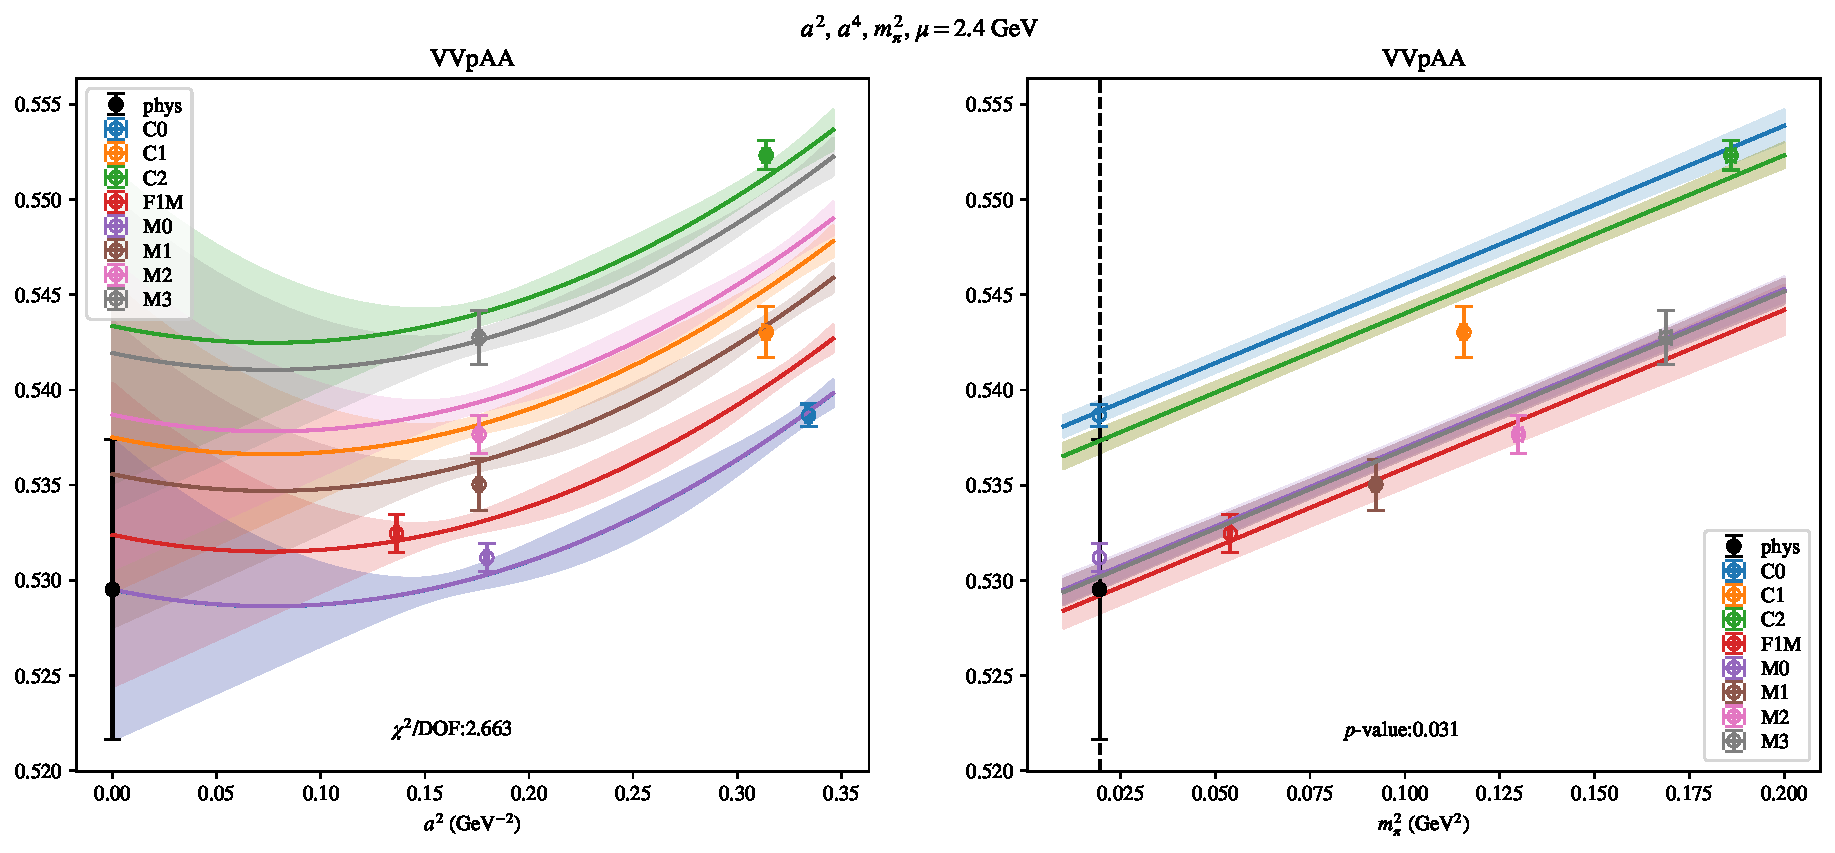
\includepdf[link, pages=-]{VVpAA/SUSY/a2a4m2_24.pdf}
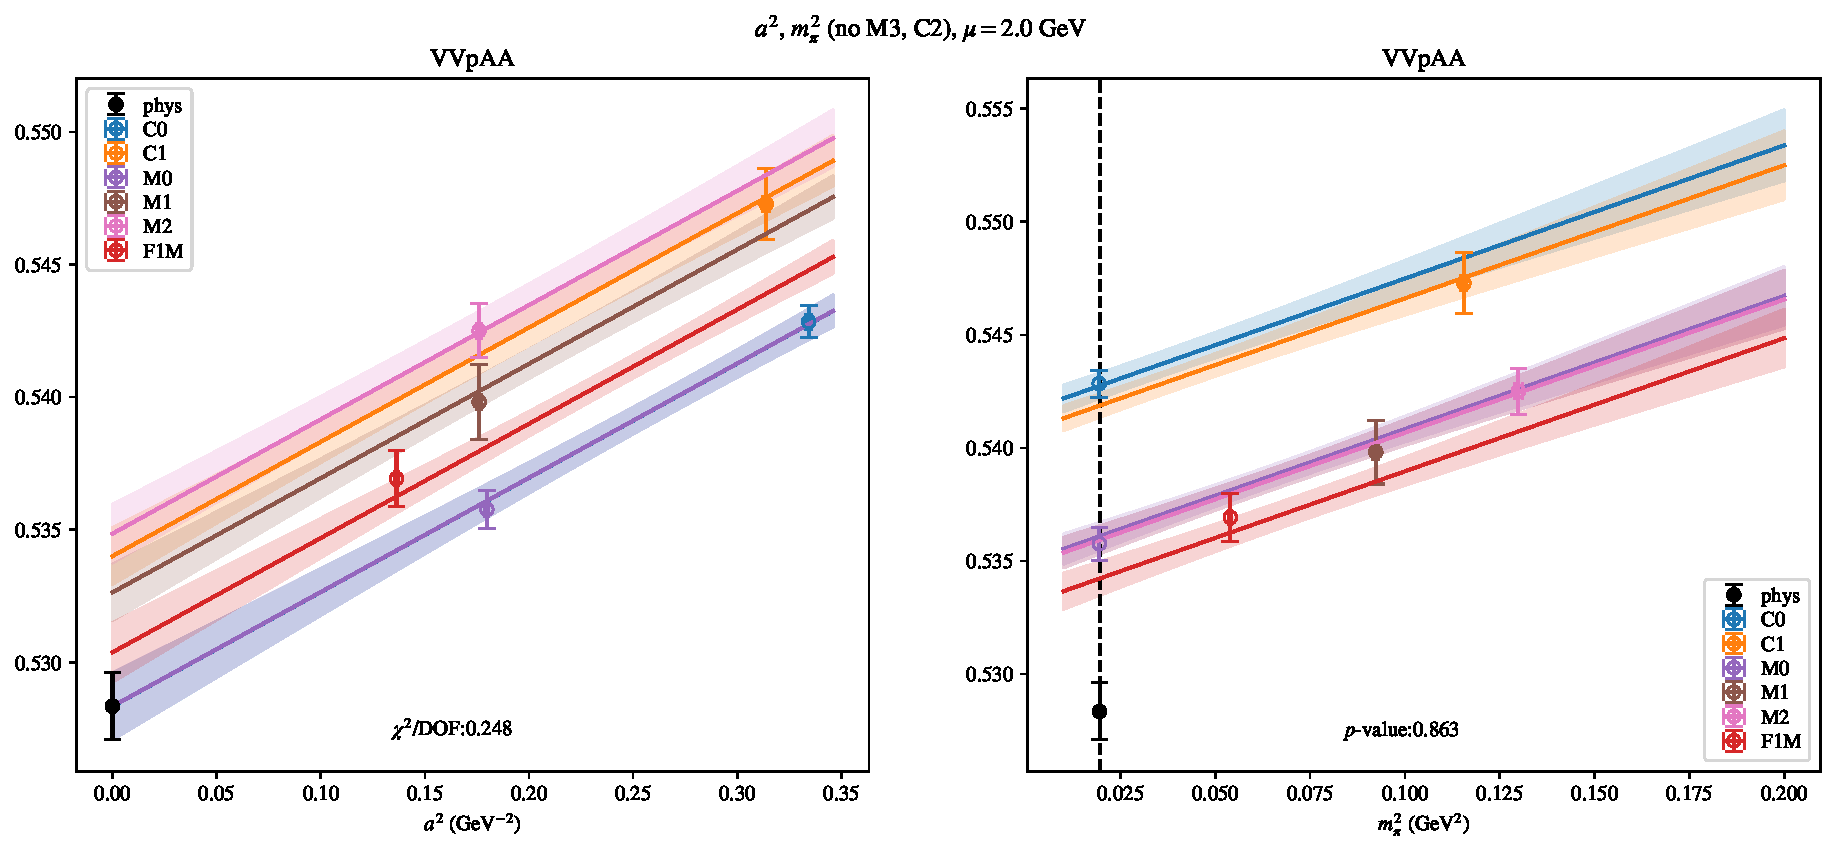
\includepdf[link, pages=-]{VVpAA/SUSY/a2m2mcut_20.pdf}
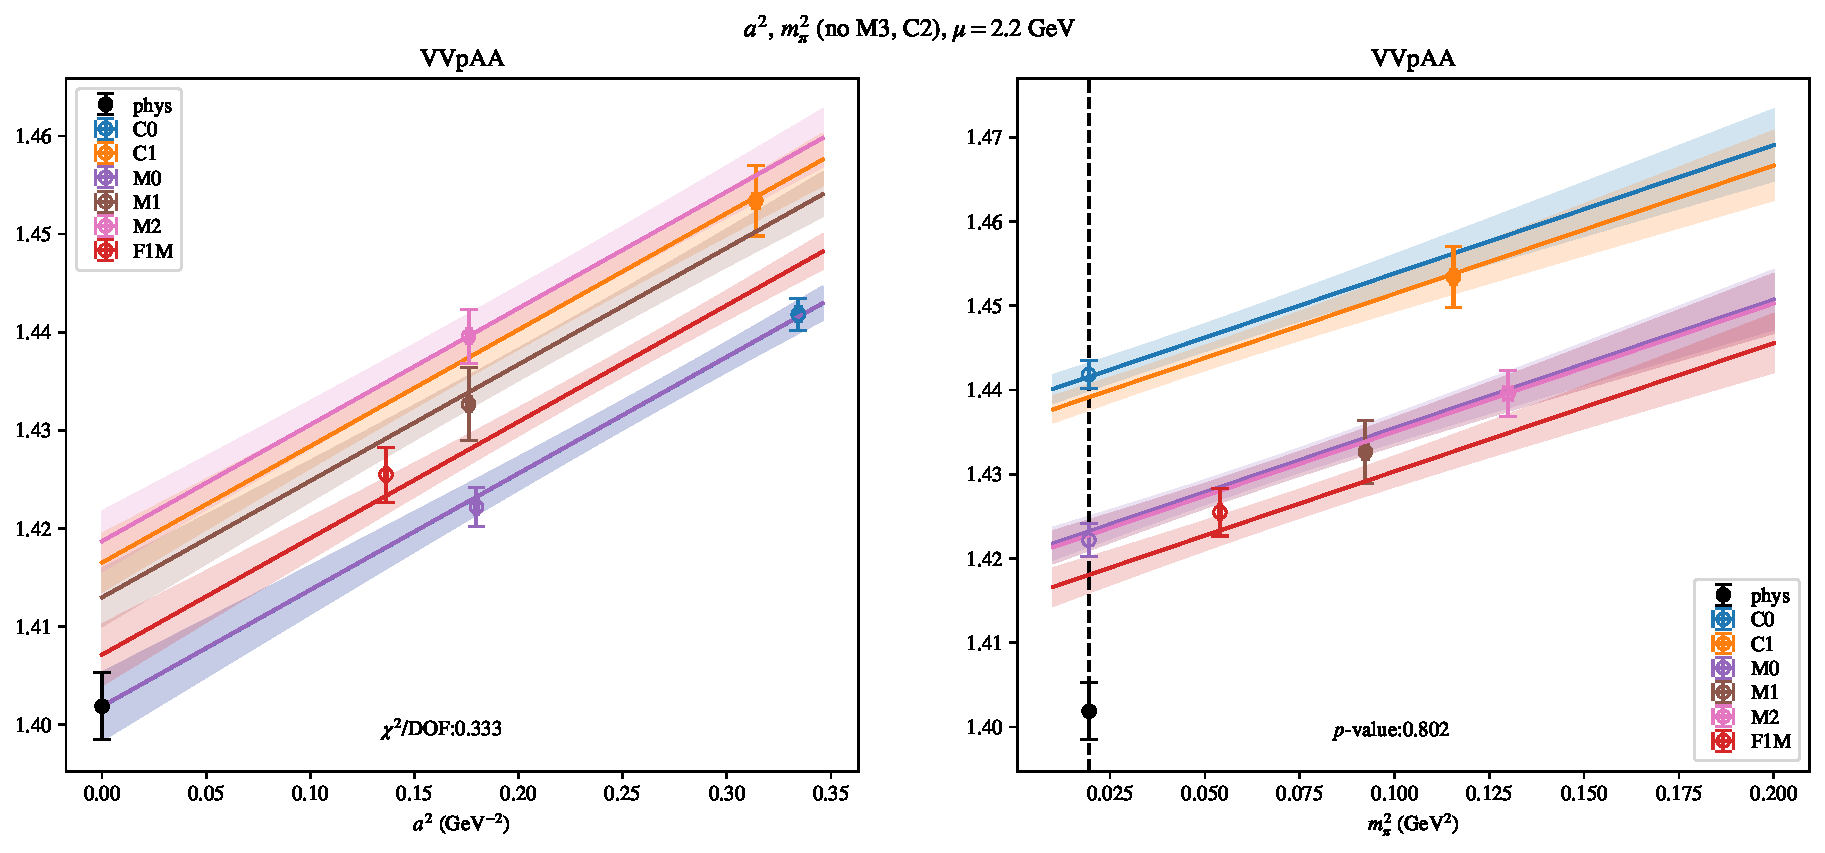
\includepdf[link, pages=-]{VVpAA/SUSY/a2m2mcut_22.pdf}
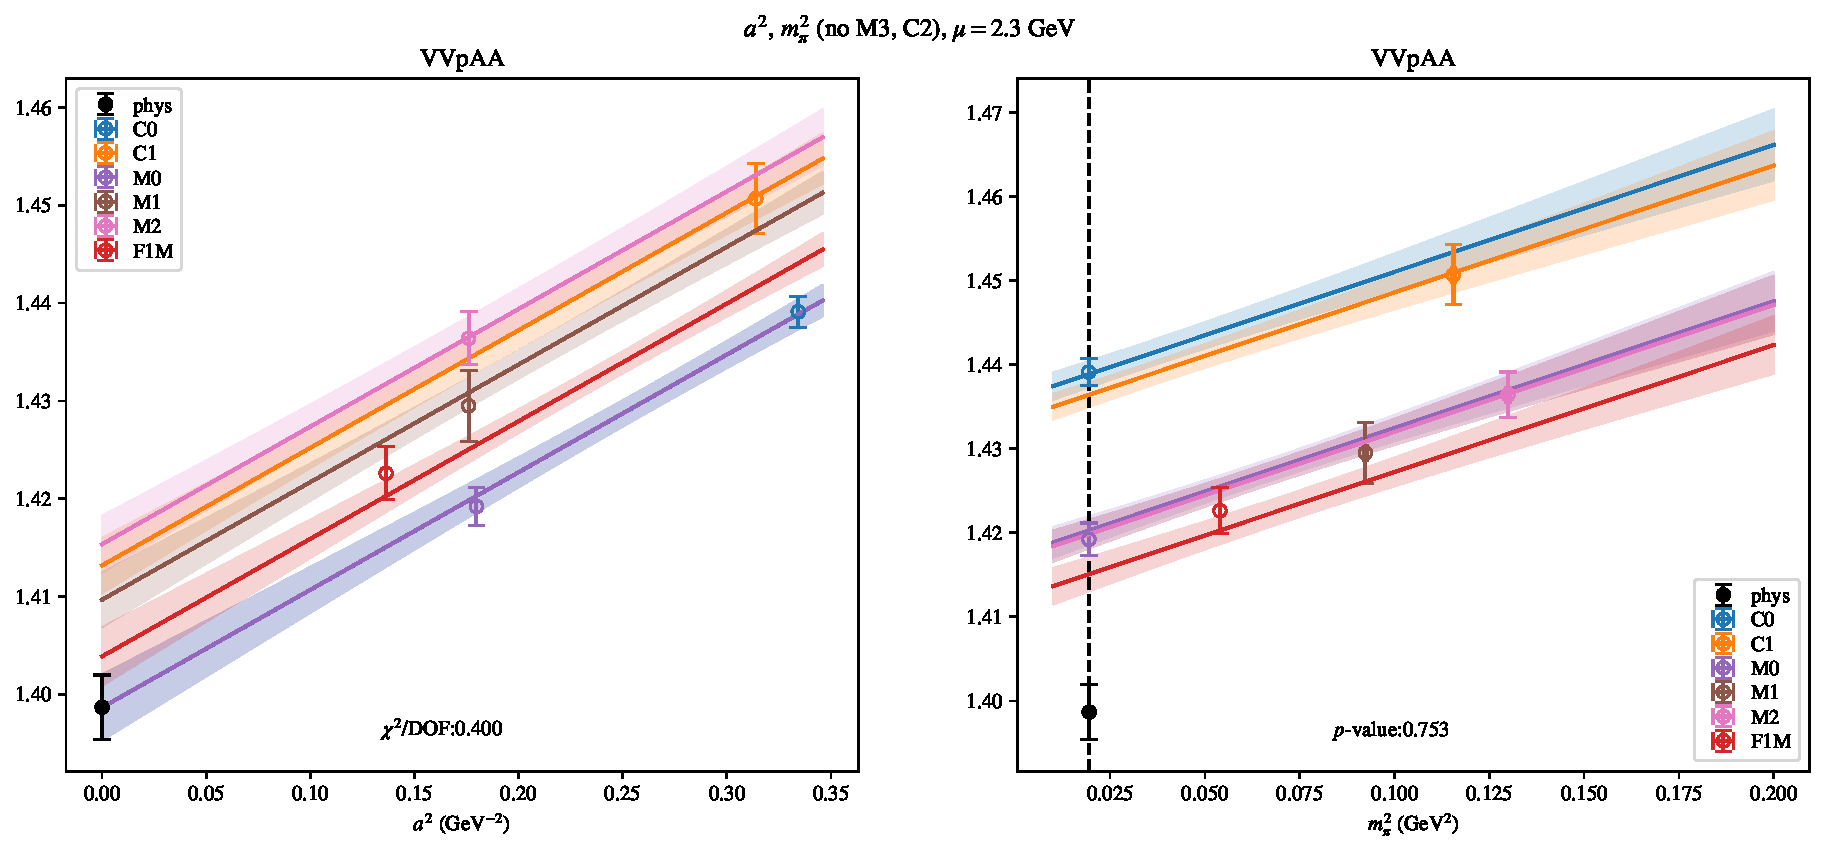
\includepdf[link, pages=-]{VVpAA/SUSY/a2m2mcut_23.pdf}
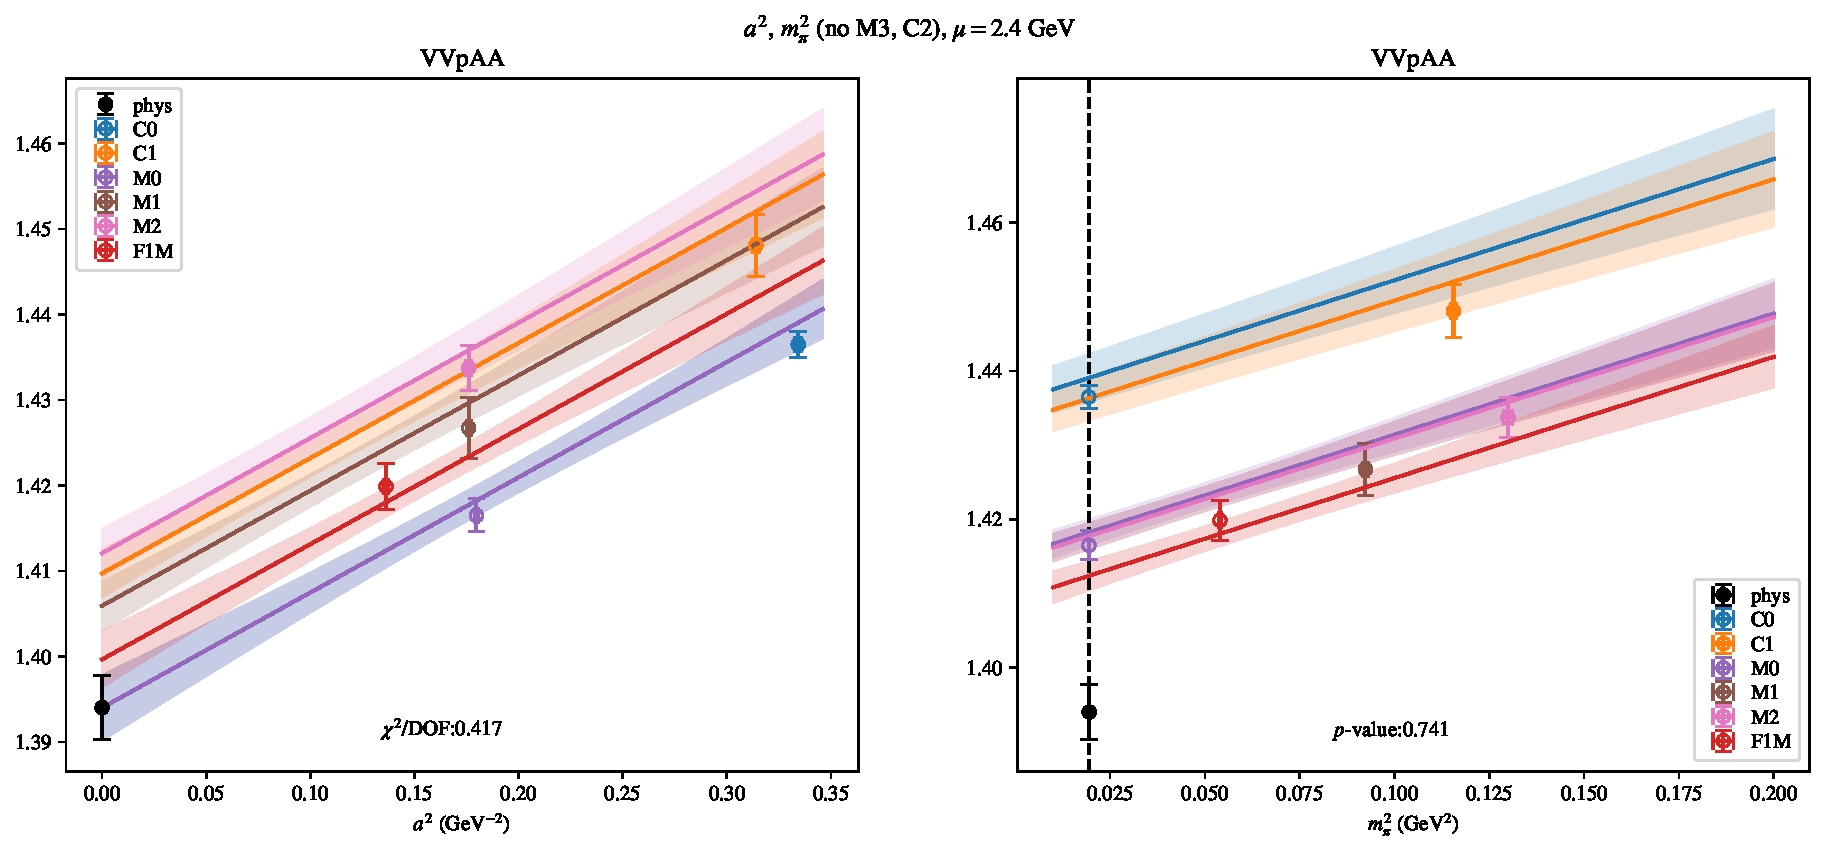
\includepdf[link, pages=-]{VVpAA/SUSY/a2m2mcut_24.pdf}
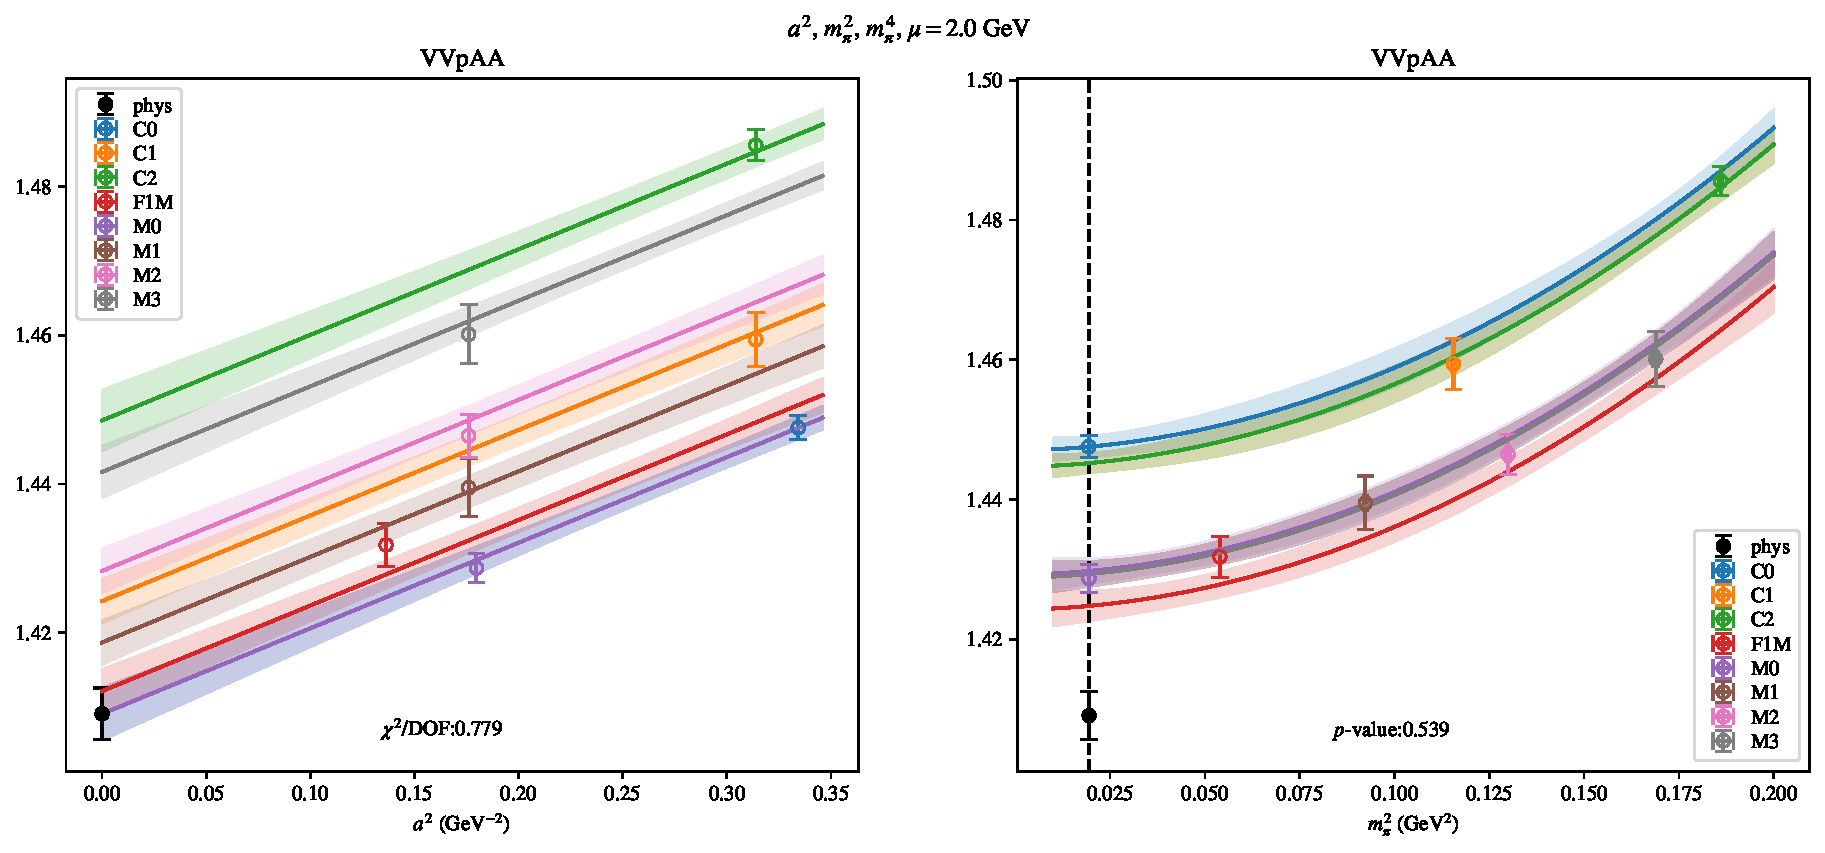
\includepdf[link, pages=-]{VVpAA/SUSY/a2m2m4_20.pdf}
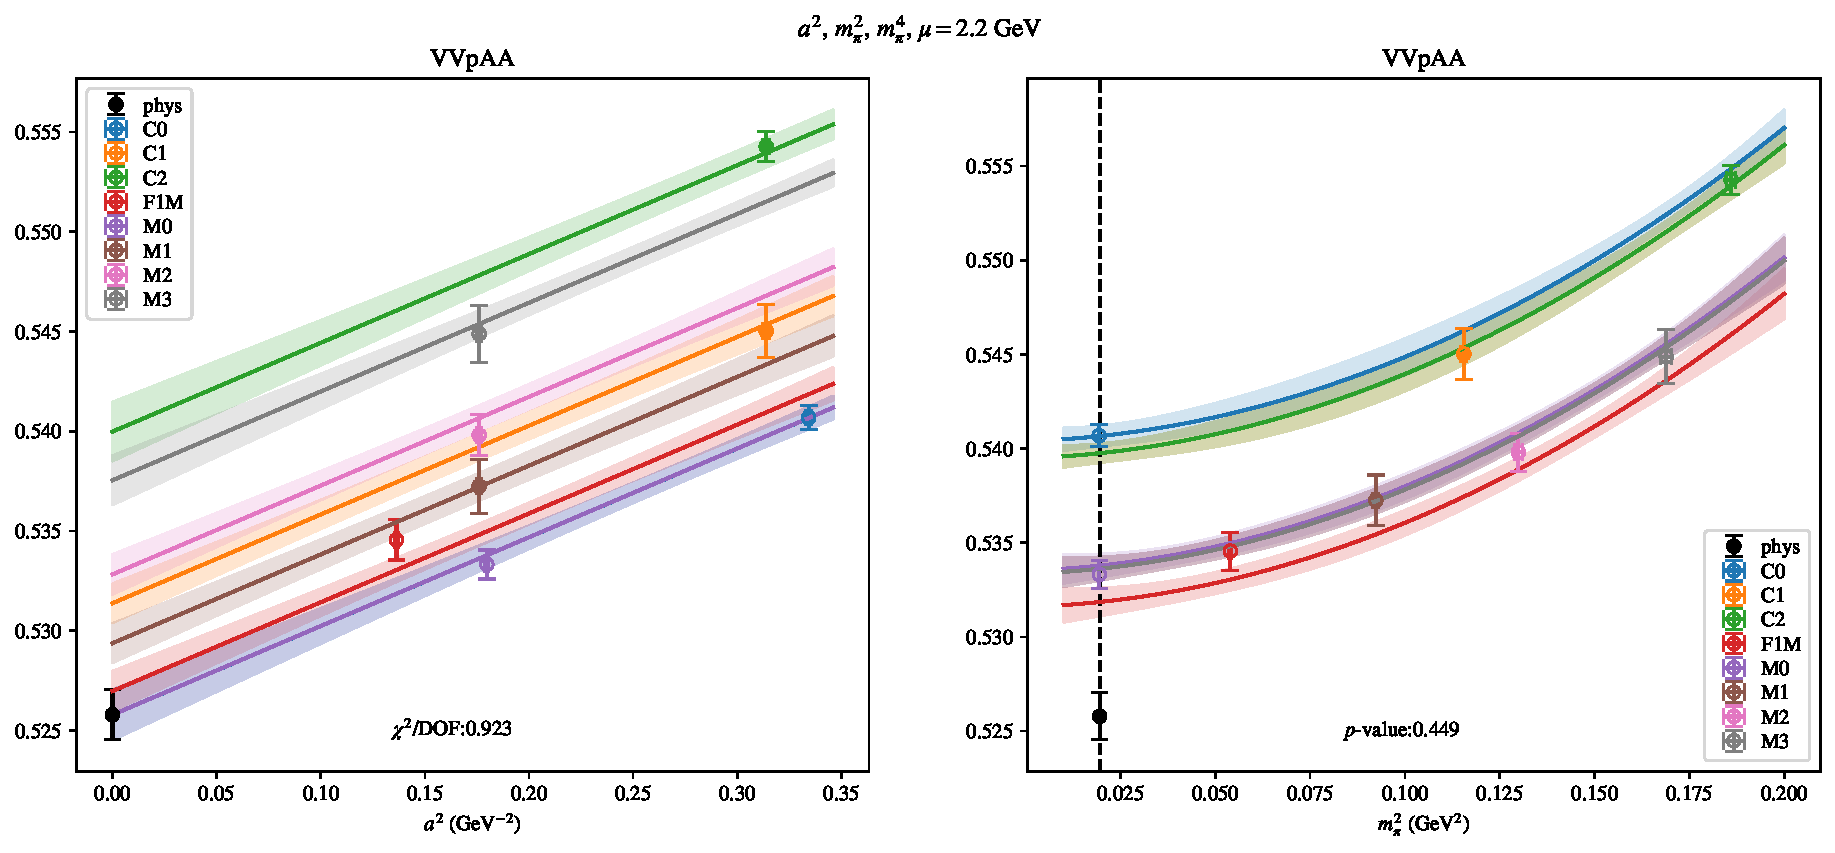
\includepdf[link, pages=-]{VVpAA/SUSY/a2m2m4_22.pdf}
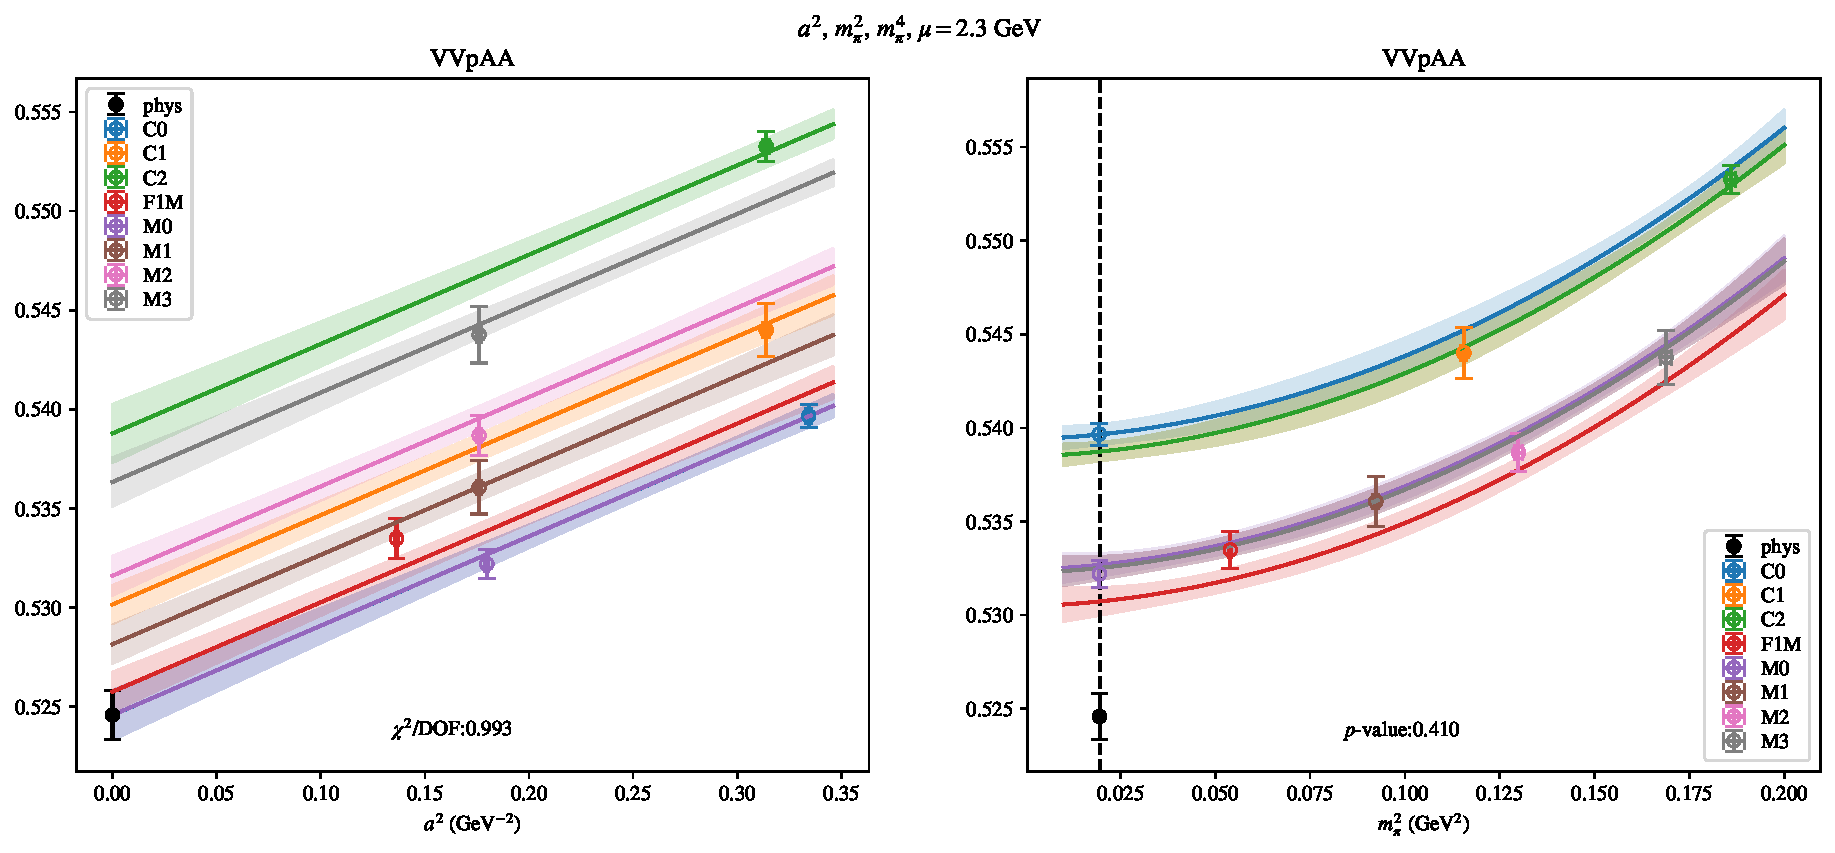
\includepdf[link, pages=-]{VVpAA/SUSY/a2m2m4_23.pdf}
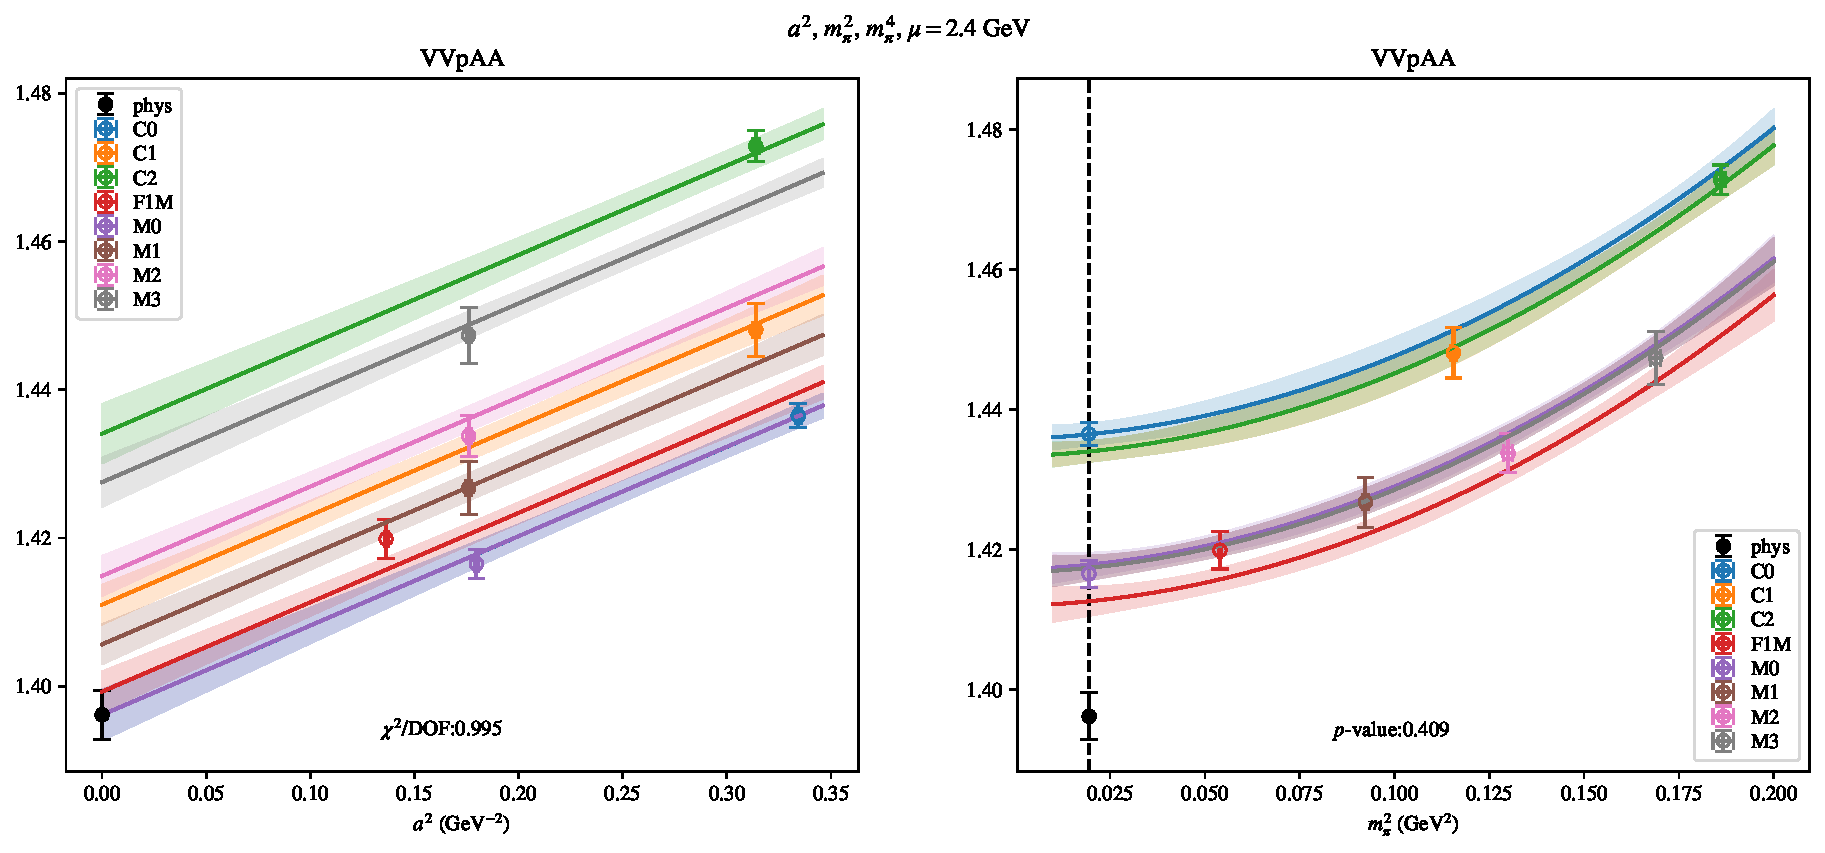
\includepdf[link, pages=-]{VVpAA/SUSY/a2m2m4_24.pdf}
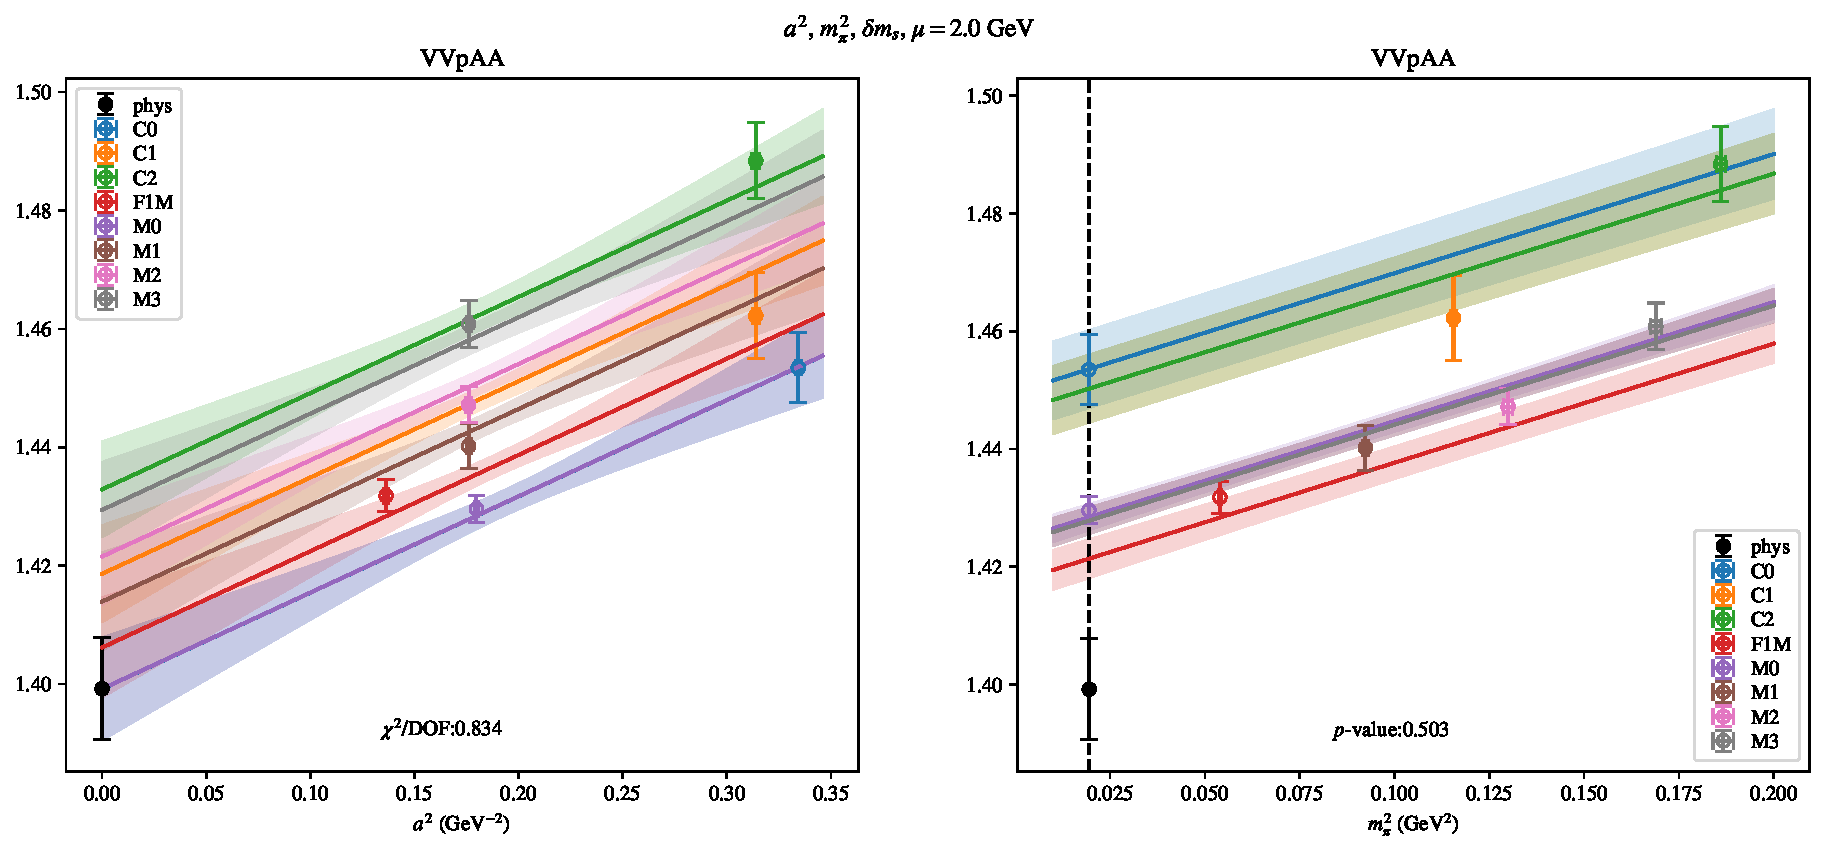
\includepdf[link, pages=-]{VVpAA/SUSY/a2m2delm_20.pdf}
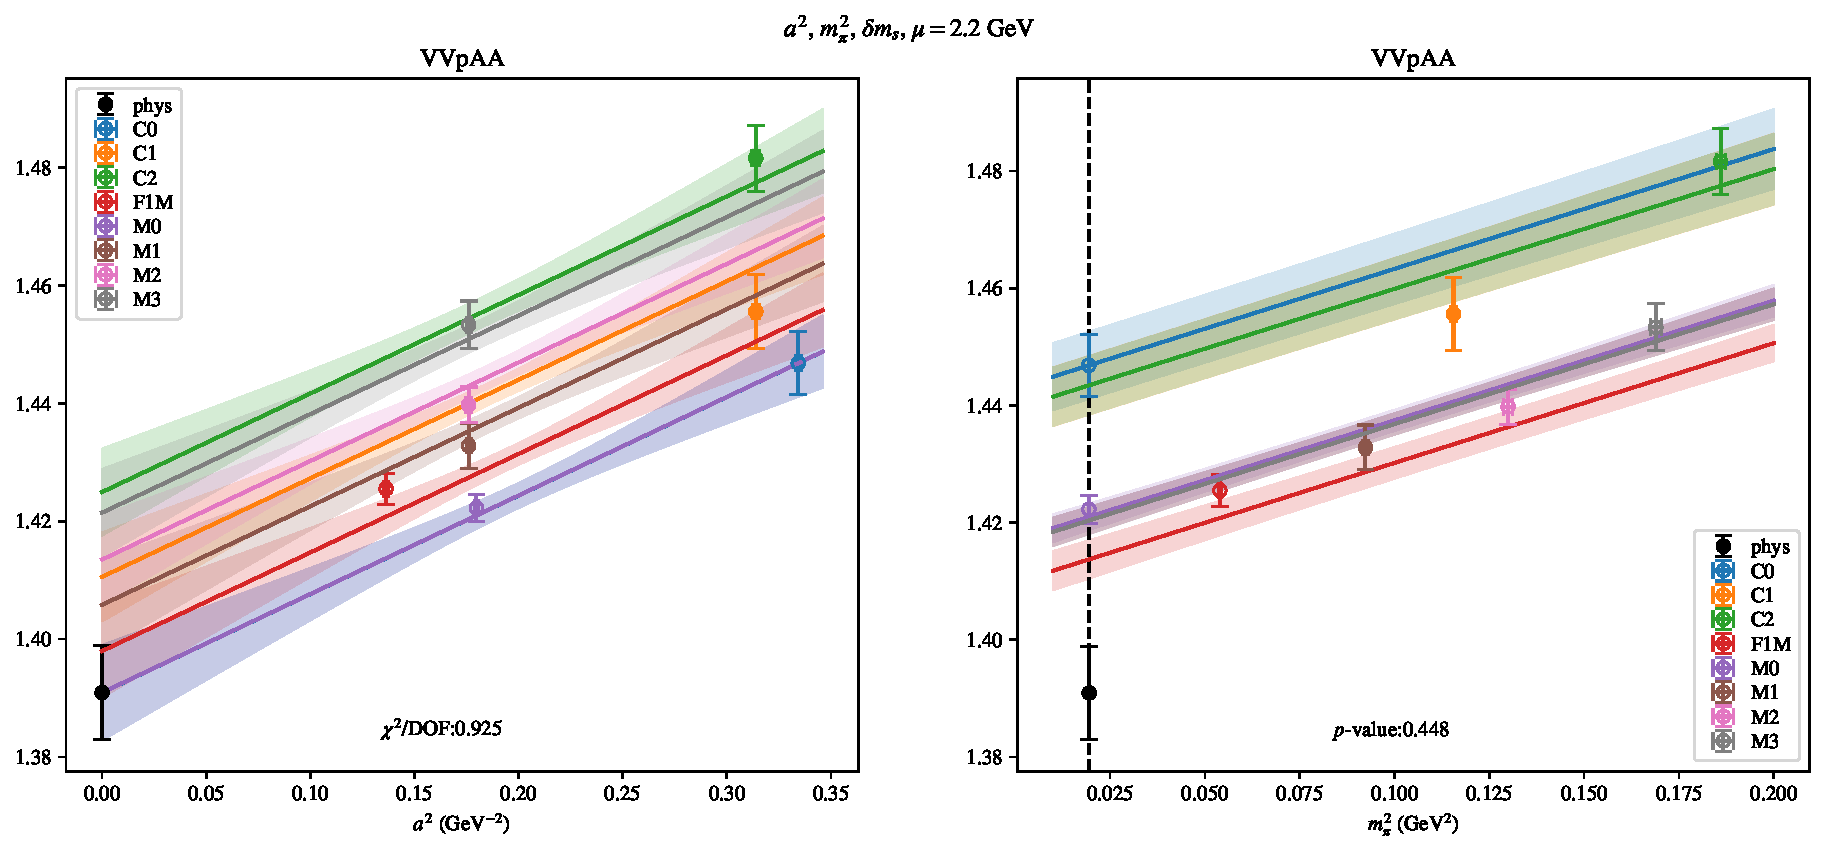
\includepdf[link, pages=-]{VVpAA/SUSY/a2m2delm_22.pdf}
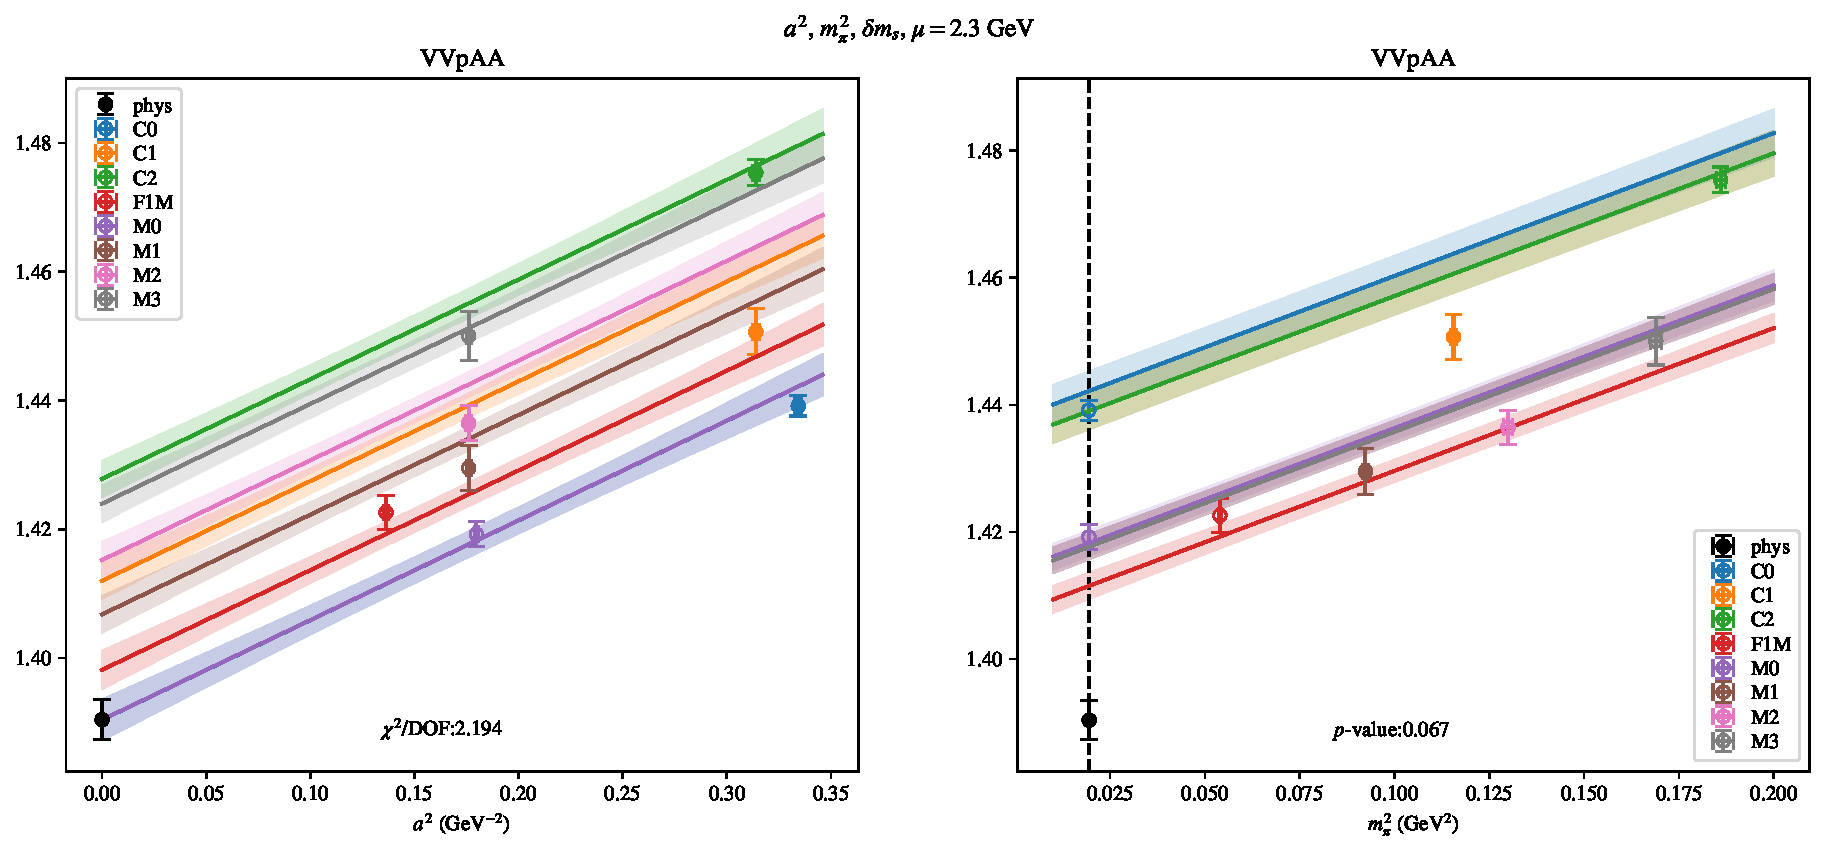
\includepdf[link, pages=-]{VVpAA/SUSY/a2m2delm_23.pdf}
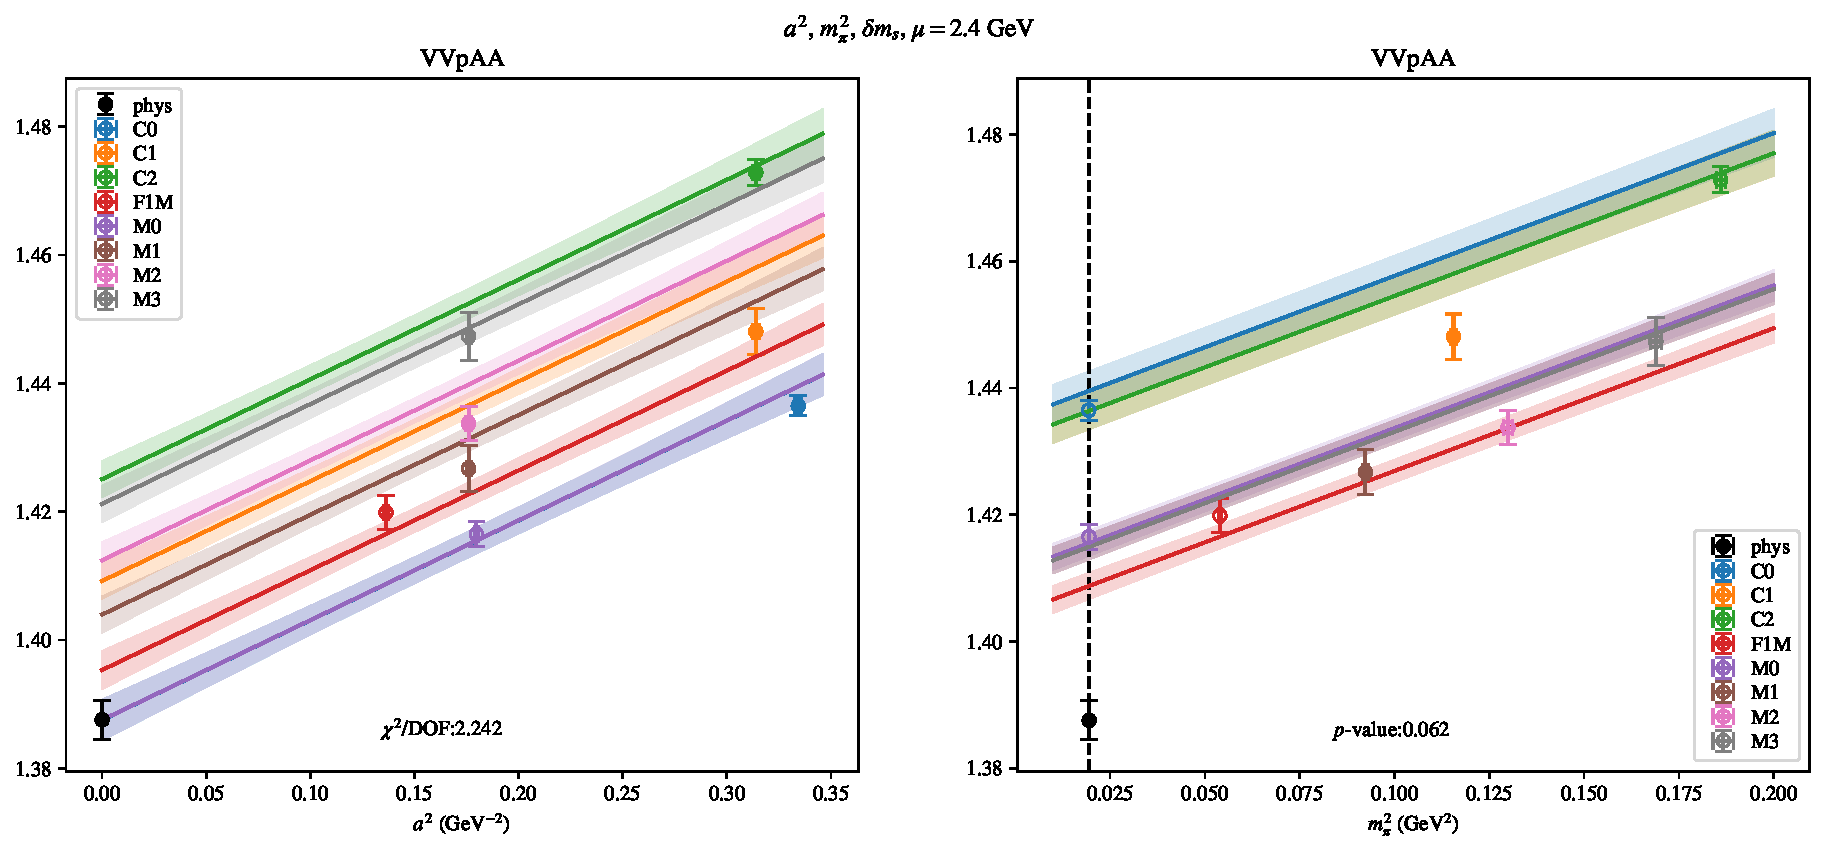
\includepdf[link, pages=-]{VVpAA/SUSY/a2m2delm_24.pdf}
\clearpage
\section{$\mathcal{B}_2$}
\begin{table}[h!]
\begin{center}
\begin{tabular}{|c|c|c|c|c|c|c|}
\hline
$\mu$ (GeV) & $a^2$, $m_\pi^2$& $a^2$, $m_\pi^2$ (no C)& $a^2$, $a^4$, $m_\pi^2$& $a^2$, $m_\pi^2$ (no M3, C2)& $a^2$, $m_\pi^2$, $m_\pi^4$& $a^2$, $m_\pi^2$, $\delta m_s$\\
\hline
2.0& \hyperlink{VVmAA/SUSY/a2m2_20.pdf.1}{\textbf{-0.926(20)}: 0.682 (0.637)} & \hyperlink{VVmAA/SUSY/a2m2noC_20.pdf.1}{\textbf{-0.92(11)}: 0.745 (0.475)} & \hyperlink{VVmAA/SUSY/a2a4m2_20.pdf.1}{\textbf{-0.92(17)}: 0.837 (0.501)} & \hyperlink{VVmAA/SUSY/a2m2mcut_20.pdf.1}{\textbf{-0.925(20)}: 0.607 (0.61)} & \hyperlink{VVmAA/SUSY/a2m2m4_20.pdf.1}{\textbf{-0.925(21)}: 0.5 (0.736)} & \hyperlink{VVmAA/SUSY/a2m2delm_20.pdf.1}{\textbf{-0.926(23)}: 0.842 (0.498)}\\
2.2& \hyperlink{VVmAA/SUSY/a2m2_22.pdf.1}{\textbf{-0.907(19)}: 1.563 (0.167)} & \hyperlink{VVmAA/SUSY/a2m2noC_22.pdf.1}{\textbf{-0.91(10)}: 0.873 (0.418)} & \hyperlink{VVmAA/SUSY/a2a4m2_22.pdf.1}{\textbf{-0.90(16)}: 1.949 (0.099)} & \hyperlink{VVmAA/SUSY/a2m2mcut_22.pdf.1}{\textbf{-0.906(19)}: 1.505 (0.211)} & \hyperlink{VVmAA/SUSY/a2m2m4_22.pdf.1}{\textbf{-0.906(19)}: 1.198 (0.309)} & \hyperlink{VVmAA/SUSY/a2m2delm_22.pdf.1}{\textbf{-0.906(22)}: 1.867 (0.113)}\\
2.3& \hyperlink{VVmAA/SUSY/a2m2_23.pdf.1}{\textbf{-0.898(18)}: 2.247 (0.047)} & \hyperlink{VVmAA/SUSY/a2m2noC_23.pdf.1}{\textbf{-0.909(96)}: 1.109 (0.33)} & \hyperlink{VVmAA/SUSY/a2a4m2_23.pdf.1}{\textbf{-0.90(15)}: 2.796 (0.025)} & \hyperlink{VVmAA/SUSY/a2m2mcut_23.pdf.1}{\textbf{-0.897(18)}: 2.34 (0.071)} & \hyperlink{VVmAA/SUSY/a2m2m4_23.pdf.1}{\textbf{-0.896(19)}: 1.966 (0.097)} & \hyperlink{VVmAA/SUSY/a2m2delm_23.pdf.1}{\textbf{-0.897(21)}: 2.618 (0.033)}\\
2.4& \hyperlink{VVmAA/SUSY/a2m2_24.pdf.1}{\textbf{-0.890(18)}: 2.787 (0.016)} & \hyperlink{VVmAA/SUSY/a2m2noC_24.pdf.1}{\textbf{-0.902(94)}: 1.352 (0.259)} & \hyperlink{VVmAA/SUSY/a2a4m2_24.pdf.1}{\textbf{-0.89(15)}: 3.476 (0.008)} & \hyperlink{VVmAA/SUSY/a2m2mcut_24.pdf.1}{\textbf{-0.890(18)}: 2.983 (0.03)} & \hyperlink{VVmAA/SUSY/a2m2m4_24.pdf.1}{\textbf{-0.889(19)}: 2.577 (0.036)} & \hyperlink{VVmAA/SUSY/a2m2delm_24.pdf.1}{\textbf{-0.889(20)}: 3.25 (0.011)}\\
\hline
\end{tabular}
\caption{Physical point value from chiral and continuum extrapolation at renormalisation scale $\mu$. Entries are \textbf{value(error)}: $\chi^2/\text{DOF}$ ($p$-value).}
\end{center}
\end{table}
\begin{table}[h!]
\begin{center}
\begin{tabular}{|c c|c|c|c|c|c|c|}
\hline
$\mu$ (GeV) &  & $a^2$, $m_\pi^2$& $a^2$, $m_\pi^2$ (no C)& $a^2$, $a^4$, $m_\pi^2$& $a^2$, $m_\pi^2$ (no M3, C2)& $a^2$, $m_\pi^2$, $m_\pi^4$& $a^2$, $m_\pi^2$, $\delta m_s$\\
\hline
\multirow{2}{0.5in}{2.0} & $\alpha$ & 0.3720(95)& 0.374(77)& 0.41(18)& 0.3736(94)& 0.3752(97)& 0.371(10)\\
 & $\beta$ & 0.00768(37)& 0.00760(83)& 0.00771(41)& 0.00817(54)& 0.0092(11)& 0.00768(37)\\
\hline
\multirow{2}{0.5in}{2.2} & $\alpha$ & 0.4163(93)& 0.358(67)& 0.39(16)& 0.4168(93)& 0.4206(95)& 0.418(10)\\
 & $\beta$ & 0.00749(23)& 0.00700(54)& 0.00747(25)& 0.00794(38)& 0.00922(94)& 0.00751(23)\\
\hline
\multirow{2}{0.5in}{2.3} & $\alpha$ & 0.4398(92)& 0.363(65)& 0.40(16)& 0.4395(93)& 0.4444(95)& 0.442(10)\\
 & $\beta$ & 0.00760(21)& 0.00700(46)& 0.00758(23)& 0.00804(36)& 0.00936(92)& 0.00764(22)\\
\hline
\multirow{2}{0.5in}{2.4} & $\alpha$ & 0.4592(91)& 0.377(65)& 0.43(16)& 0.4585(93)& 0.4642(95)& 0.462(10)\\
 & $\beta$ & 0.00765(19)& 0.00701(40)& 0.00763(21)& 0.00807(34)& 0.00938(90)& 0.00769(20)\\
\hline
\end{tabular}
\caption{Fit values of coefficients in $Q = Q_{phys} + \mathbf{\alpha} a^2 + \mathbf{\beta}\left(\frac{m_\pi^2}{f_\pi^2}-\frac{m_{\pi,PDG}^2}{f_\pi^2}\right) + \ldots$.}
\end{center}
\end{table}
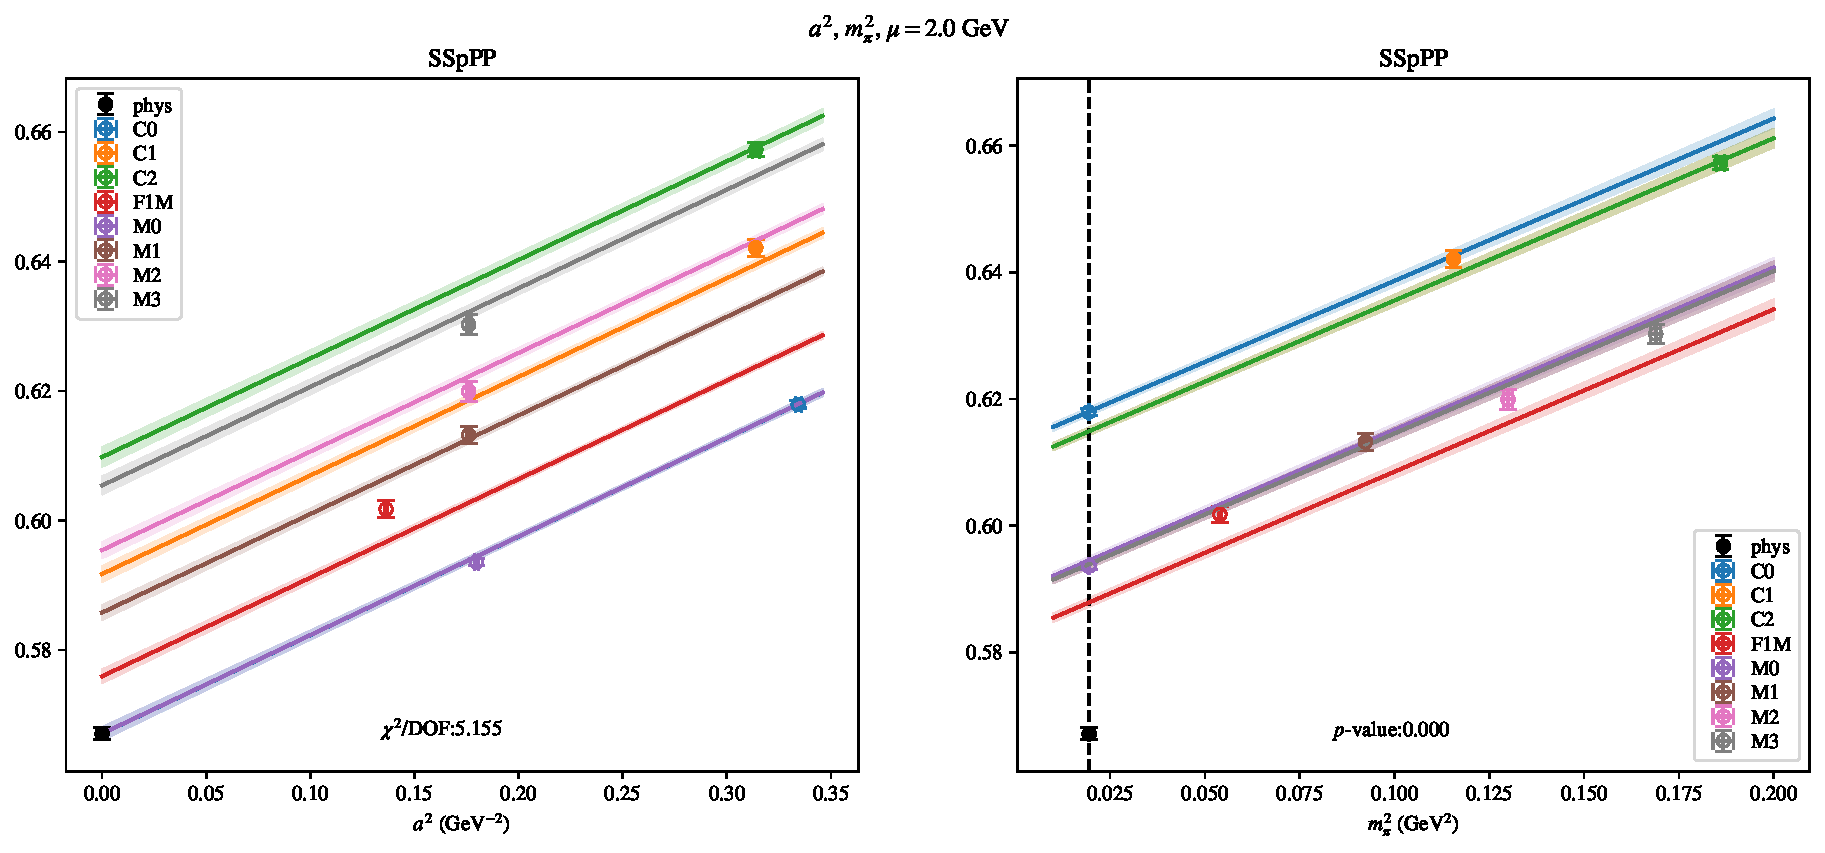
\includepdf[link, pages=-]{VVmAA/SUSY/a2m2_20.pdf}
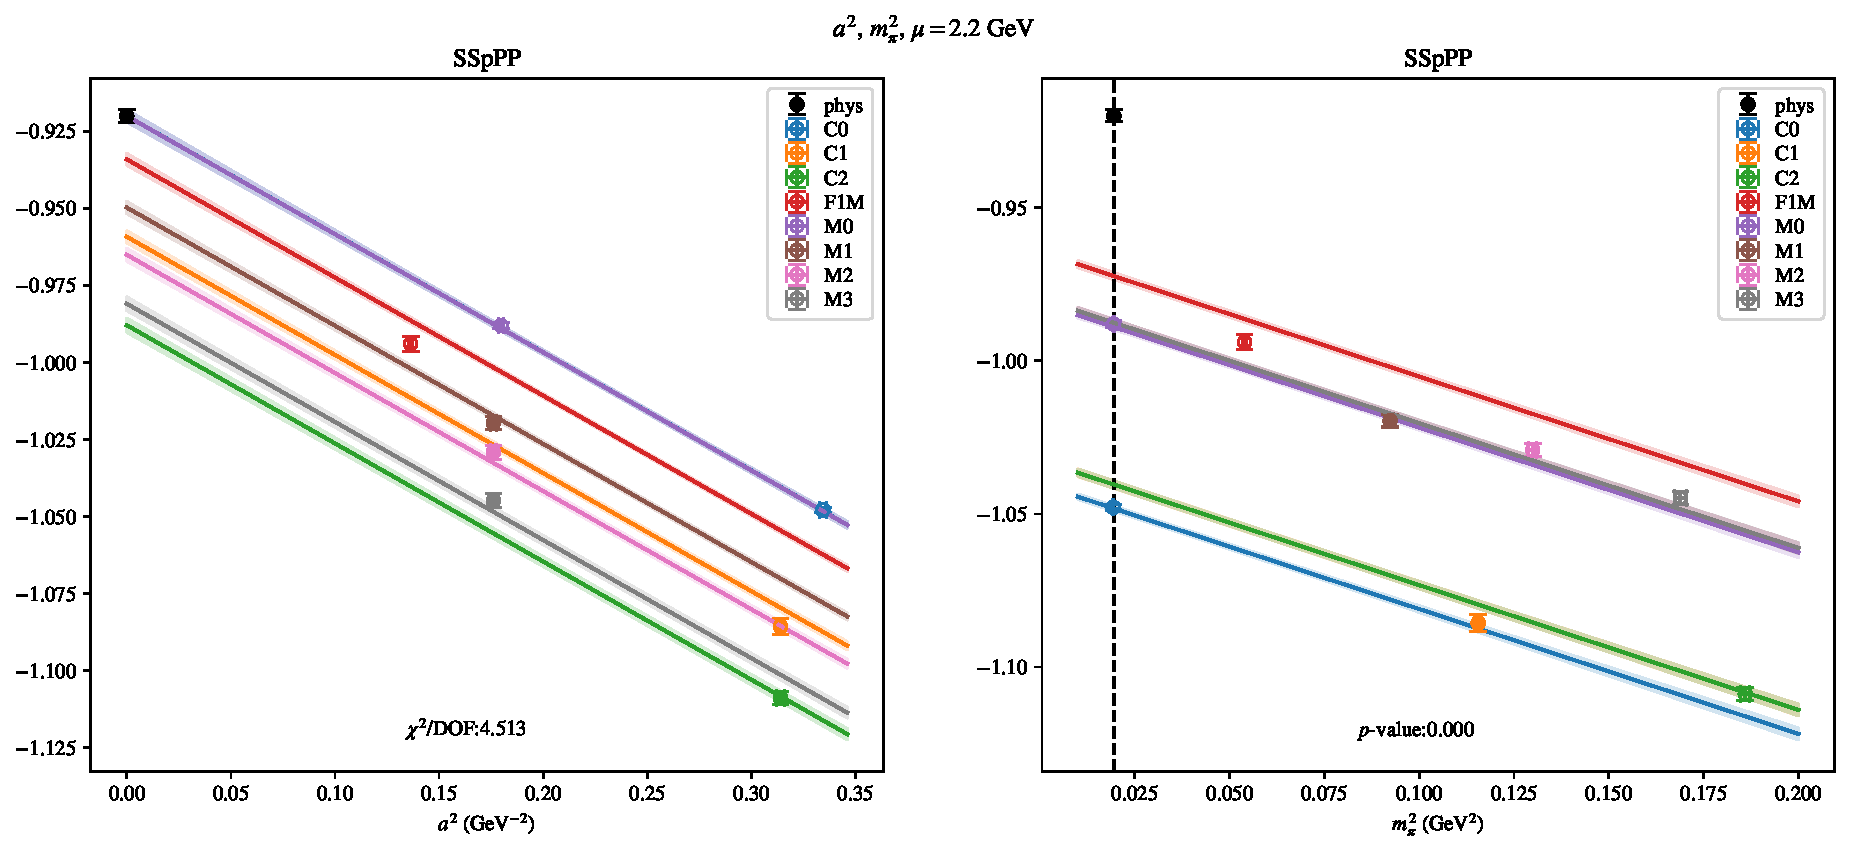
\includepdf[link, pages=-]{VVmAA/SUSY/a2m2_22.pdf}
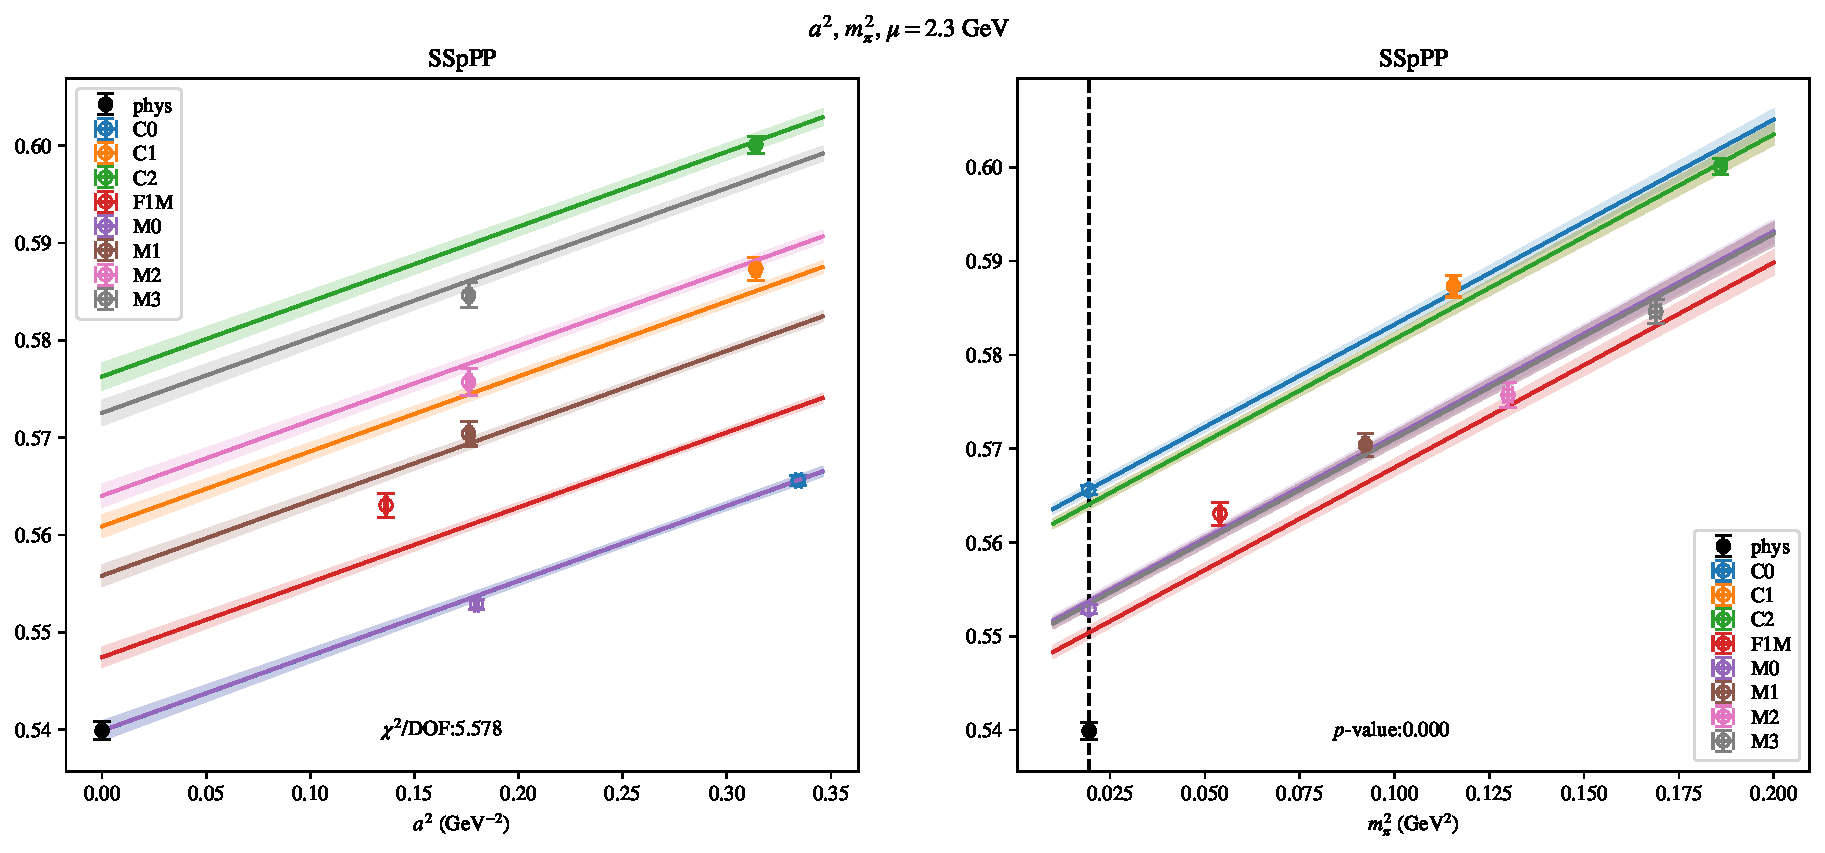
\includepdf[link, pages=-]{VVmAA/SUSY/a2m2_23.pdf}
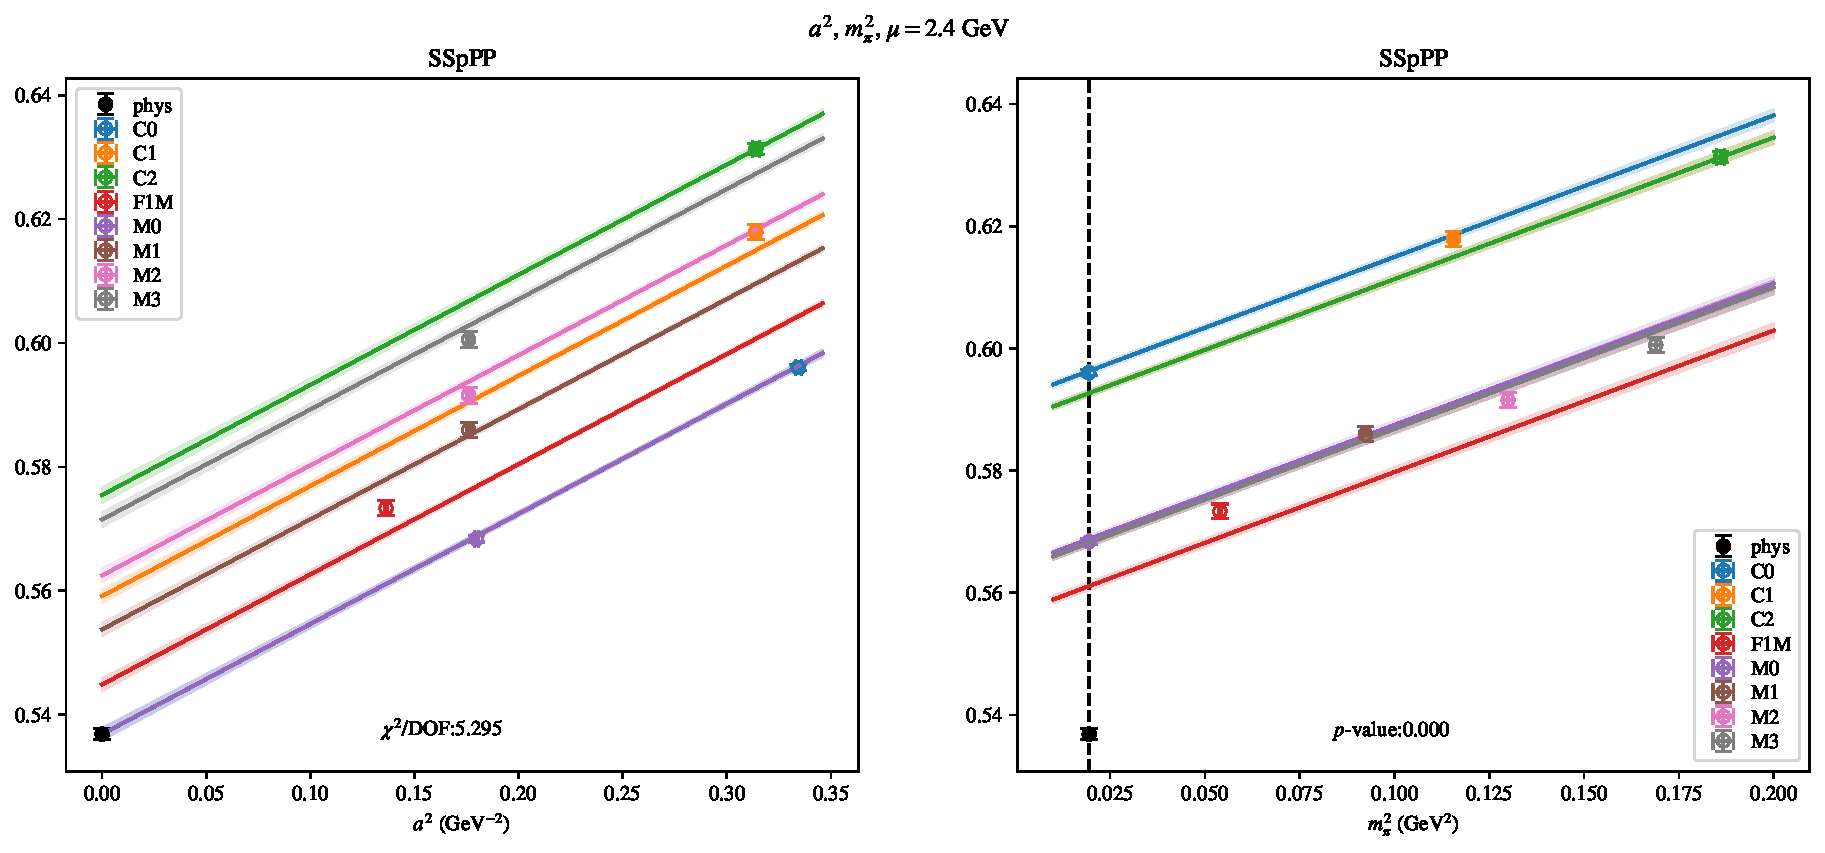
\includepdf[link, pages=-]{VVmAA/SUSY/a2m2_24.pdf}
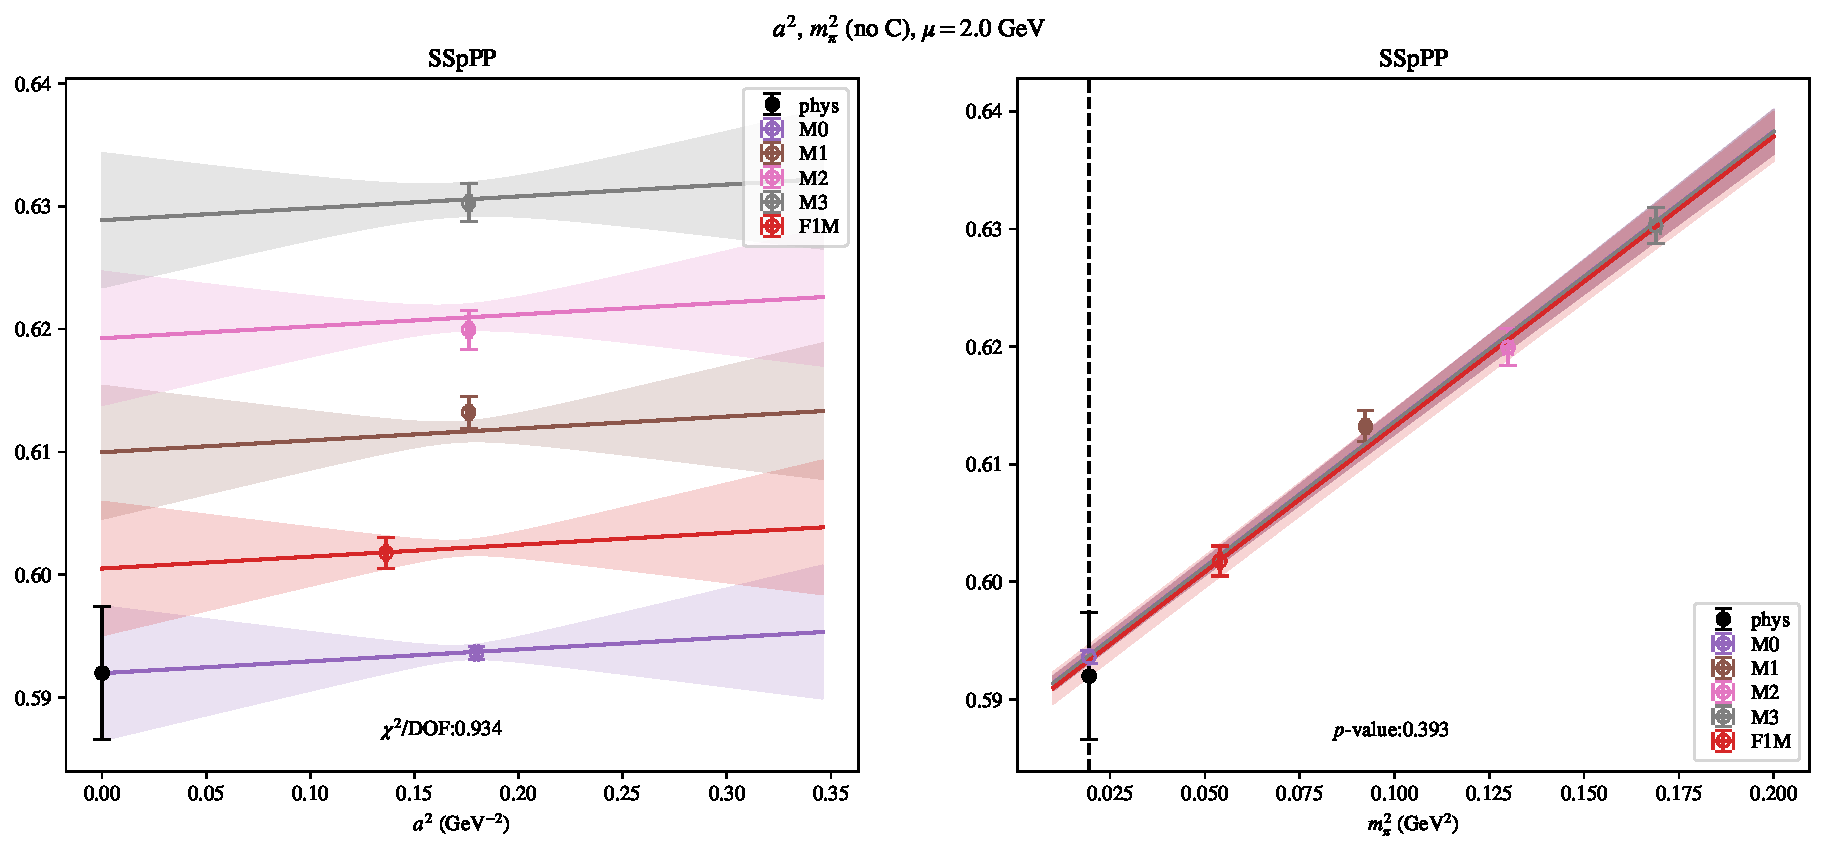
\includepdf[link, pages=-]{VVmAA/SUSY/a2m2noC_20.pdf}
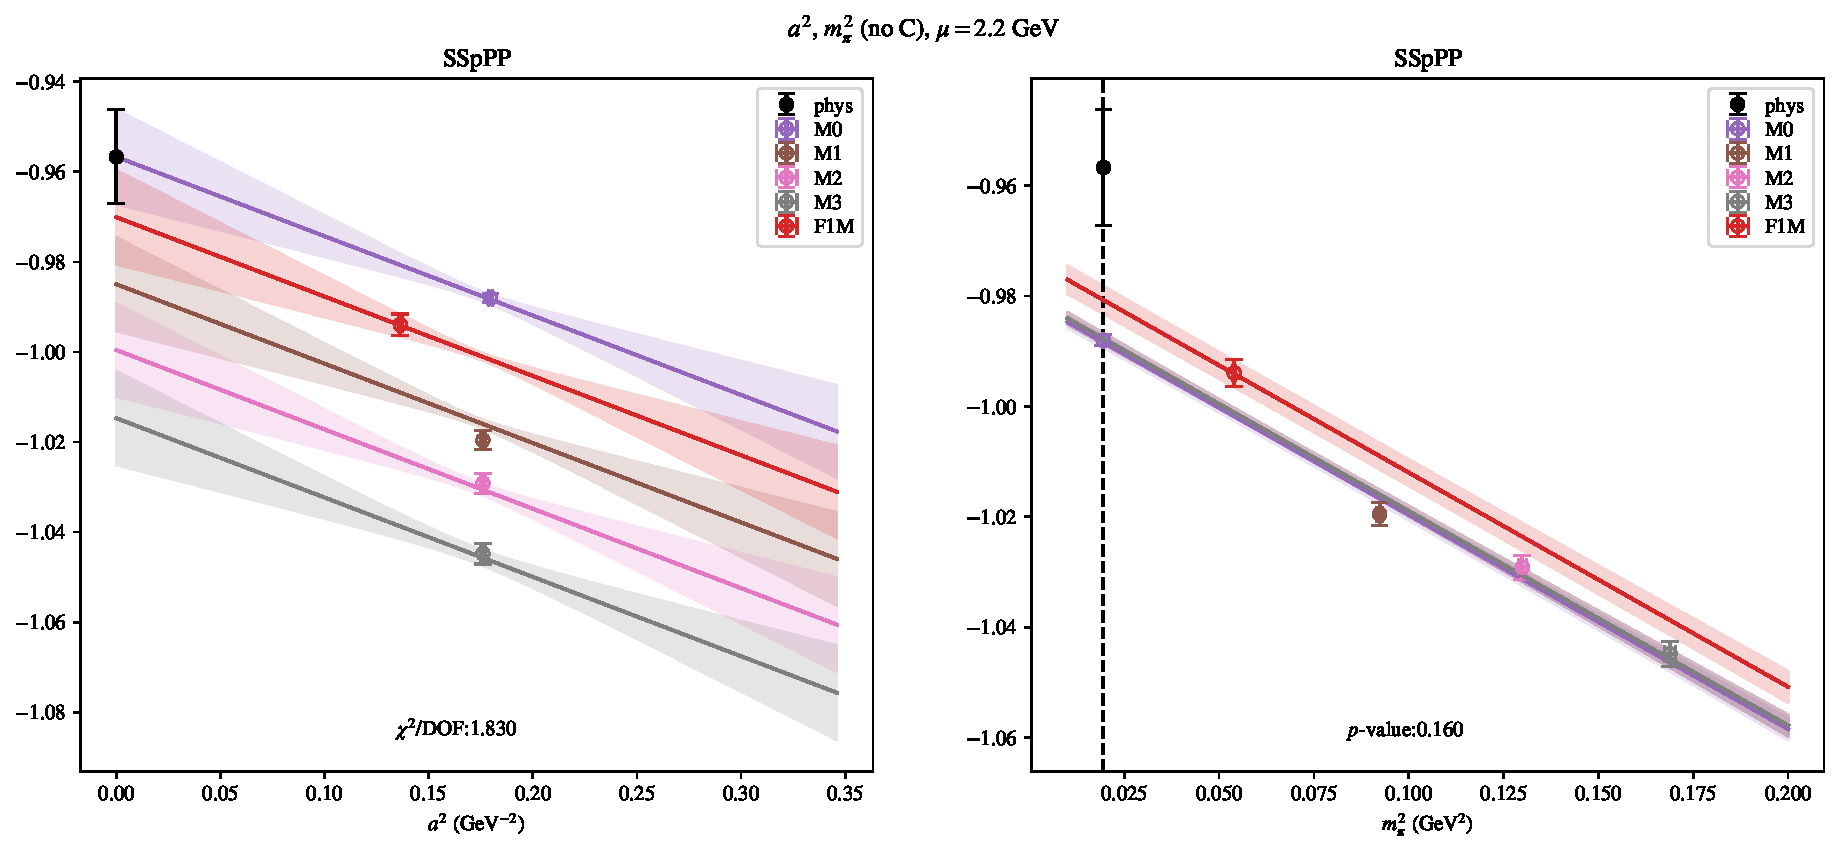
\includepdf[link, pages=-]{VVmAA/SUSY/a2m2noC_22.pdf}
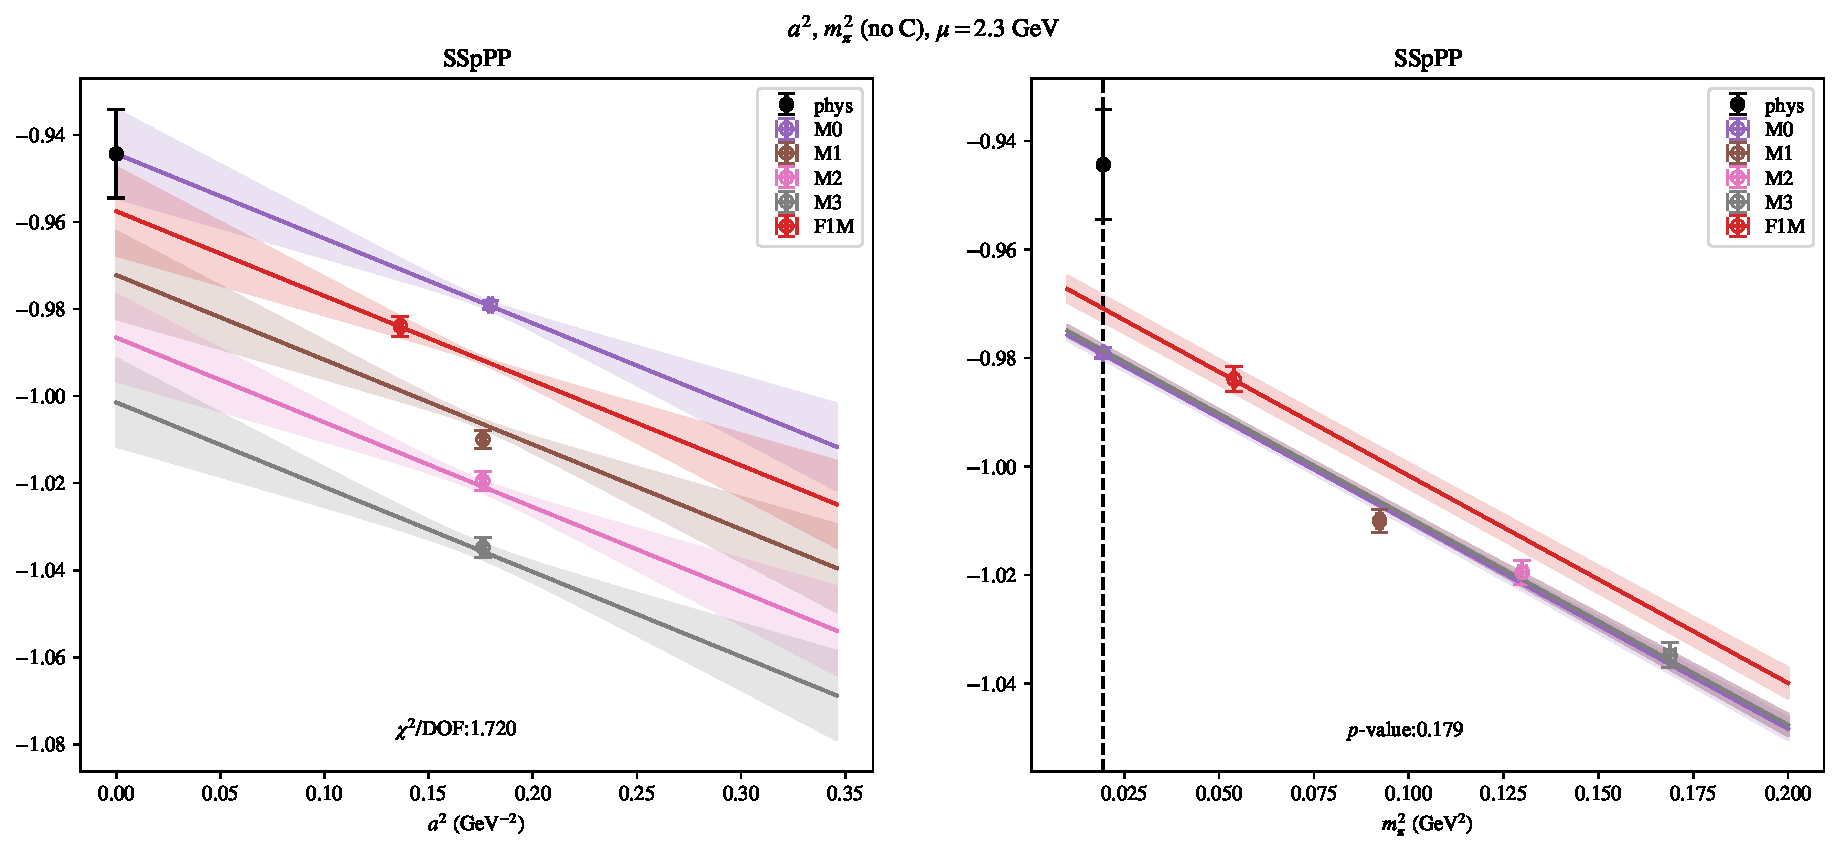
\includepdf[link, pages=-]{VVmAA/SUSY/a2m2noC_23.pdf}
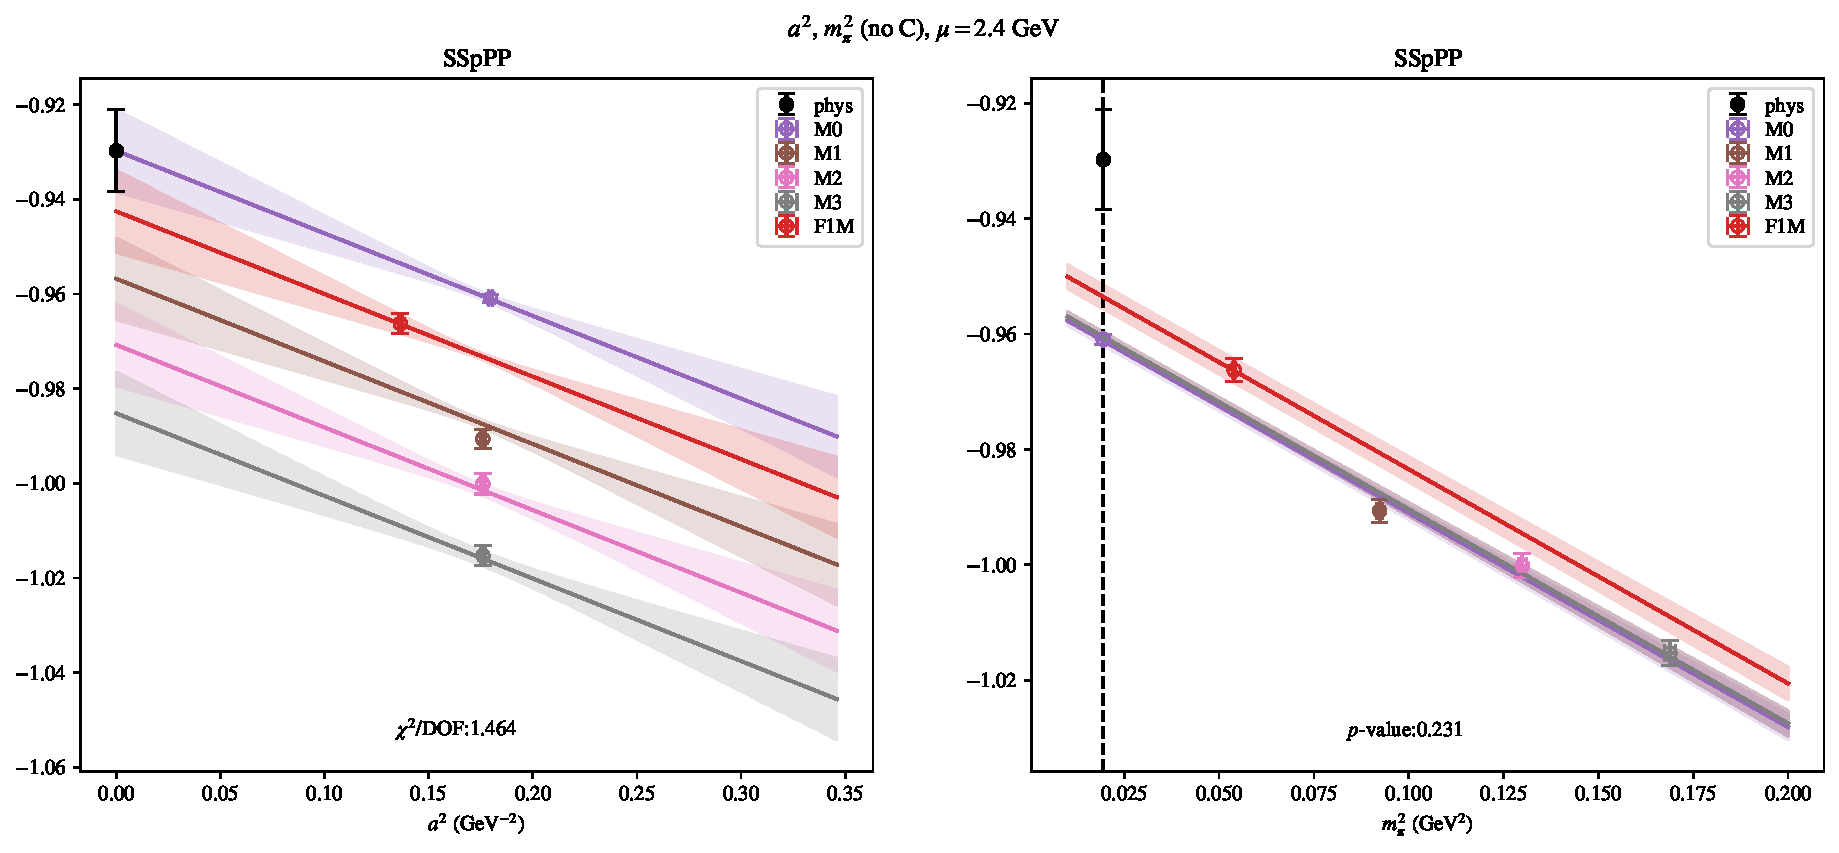
\includepdf[link, pages=-]{VVmAA/SUSY/a2m2noC_24.pdf}
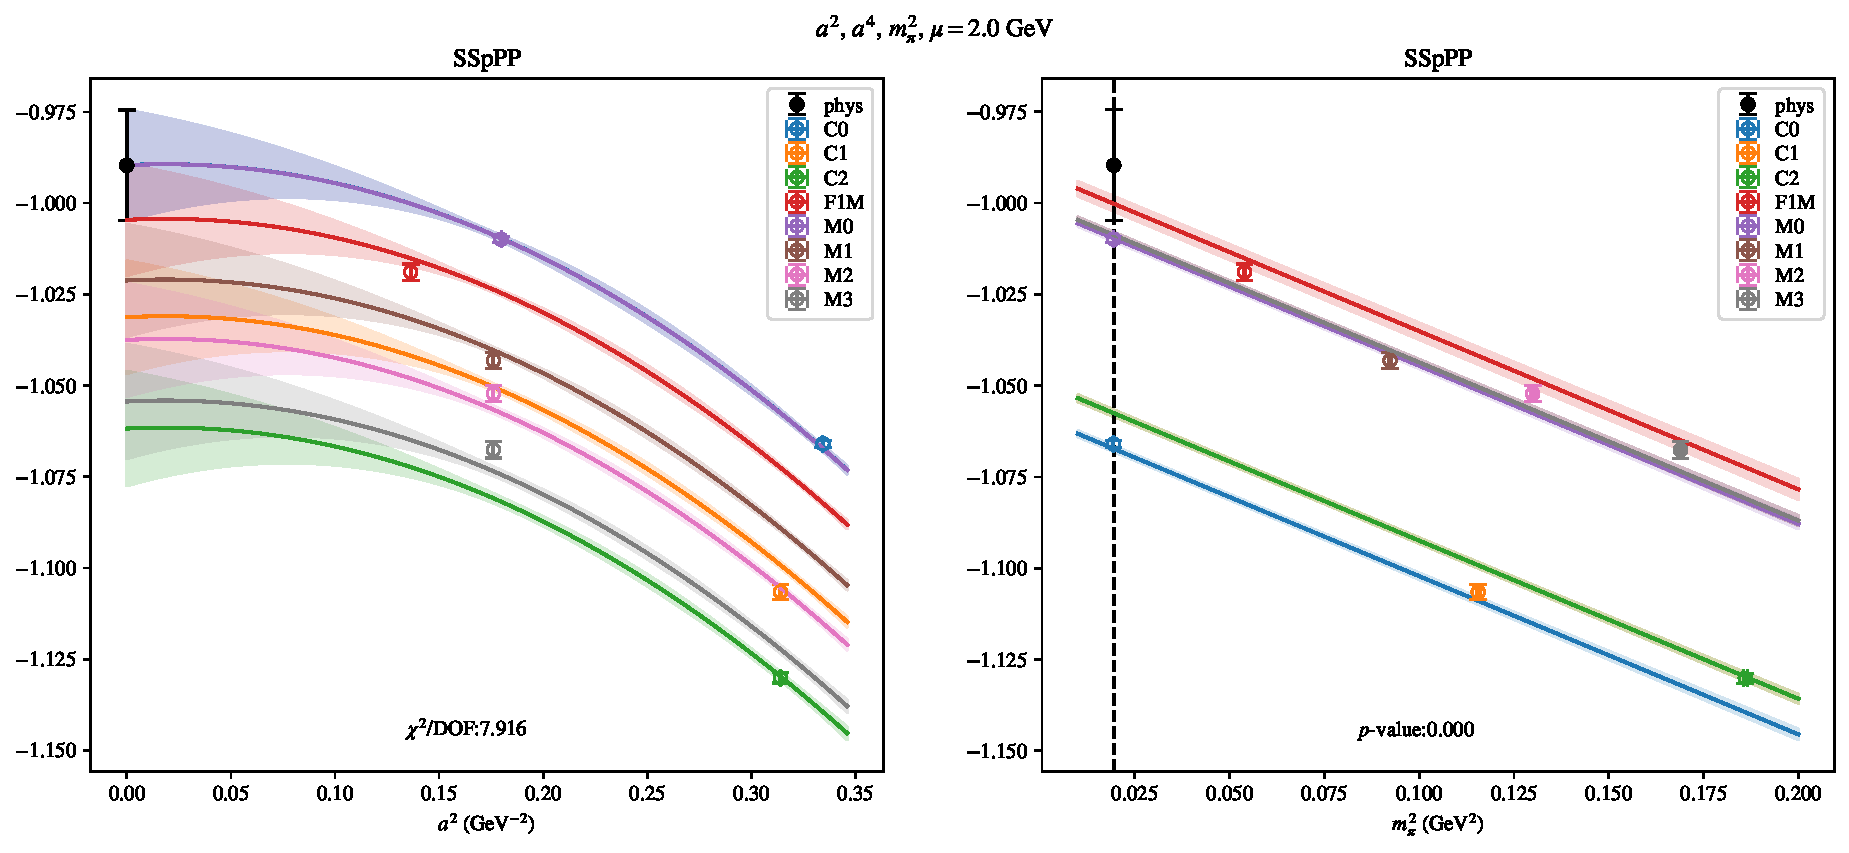
\includepdf[link, pages=-]{VVmAA/SUSY/a2a4m2_20.pdf}
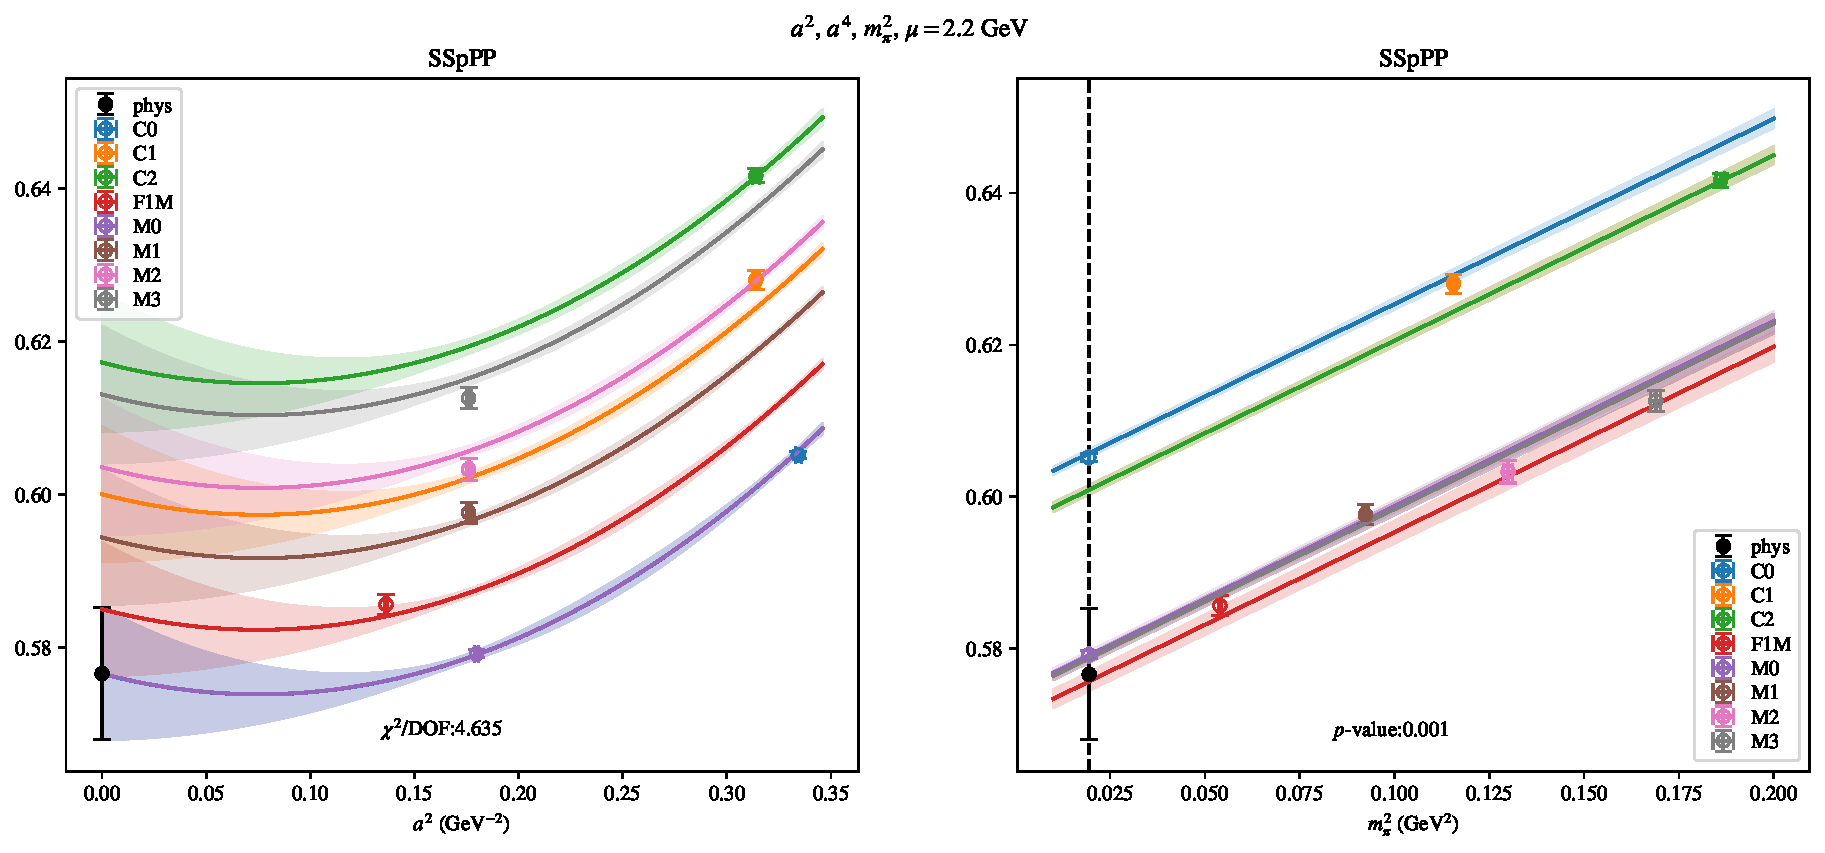
\includepdf[link, pages=-]{VVmAA/SUSY/a2a4m2_22.pdf}
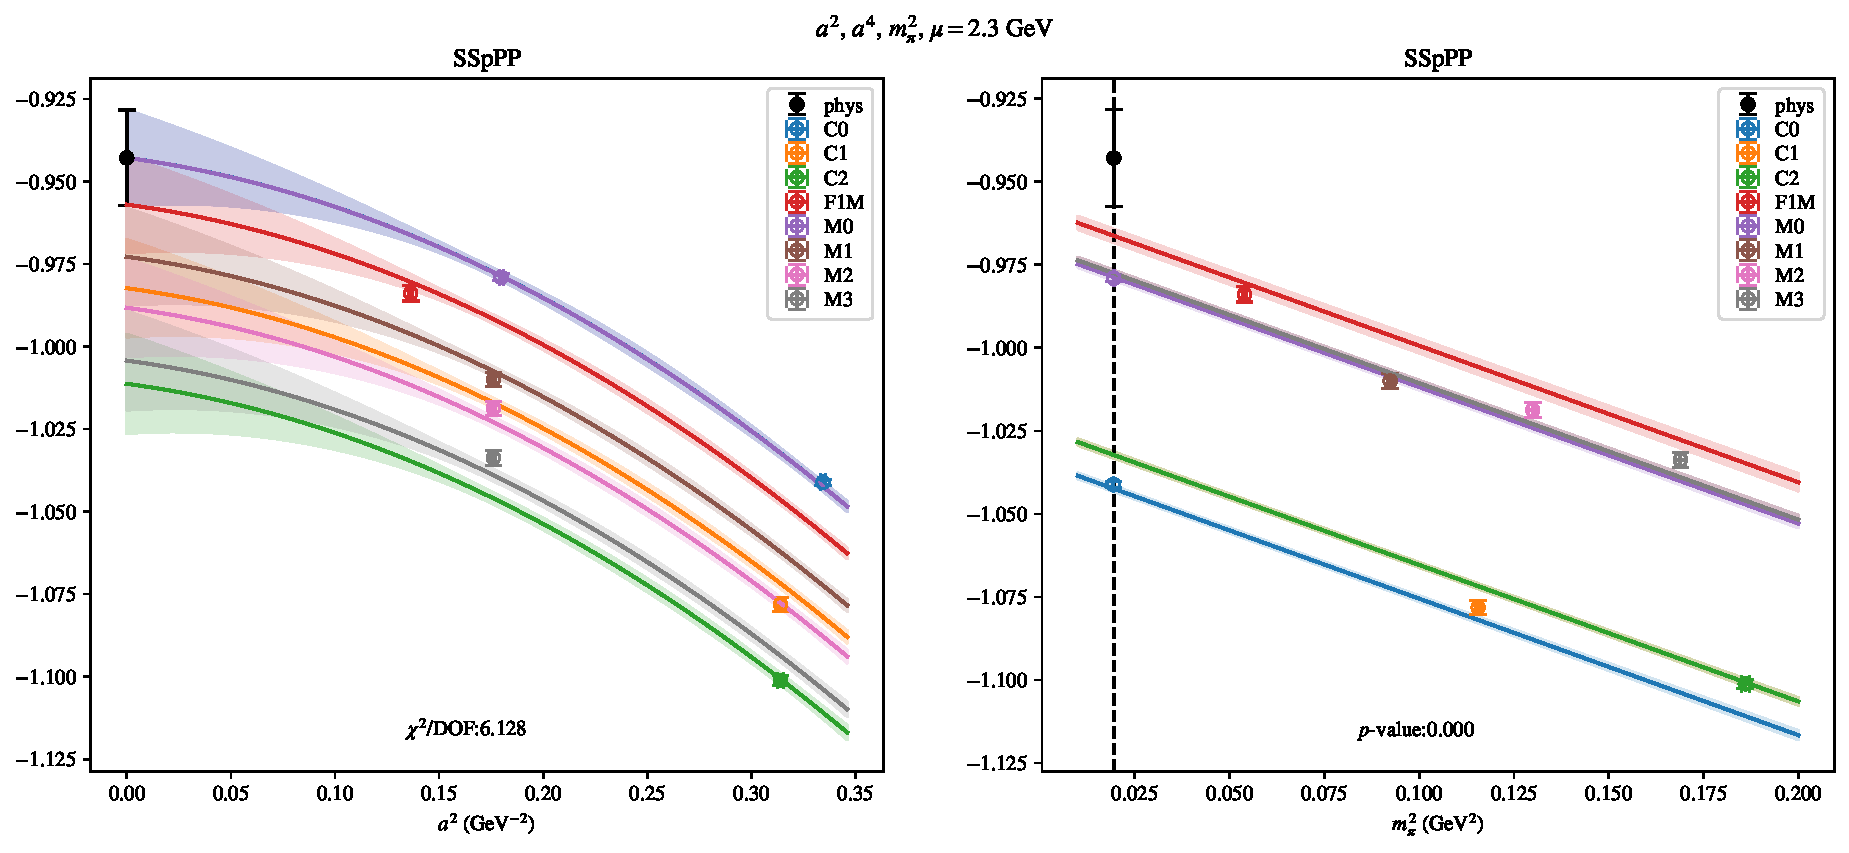
\includepdf[link, pages=-]{VVmAA/SUSY/a2a4m2_23.pdf}
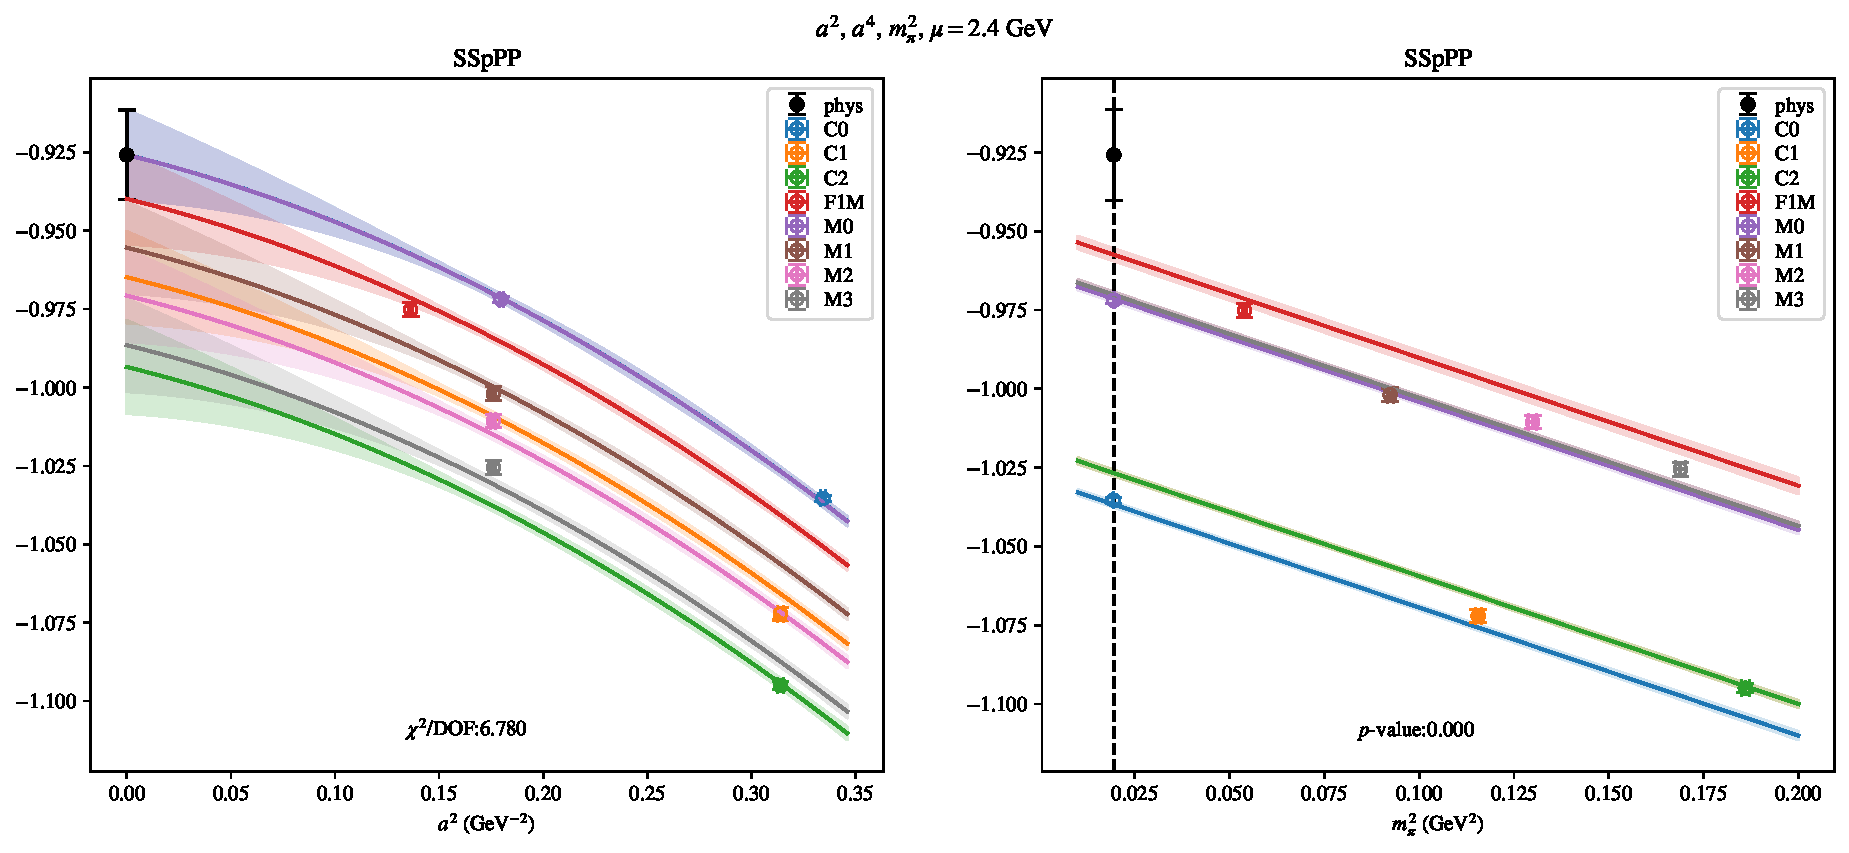
\includepdf[link, pages=-]{VVmAA/SUSY/a2a4m2_24.pdf}
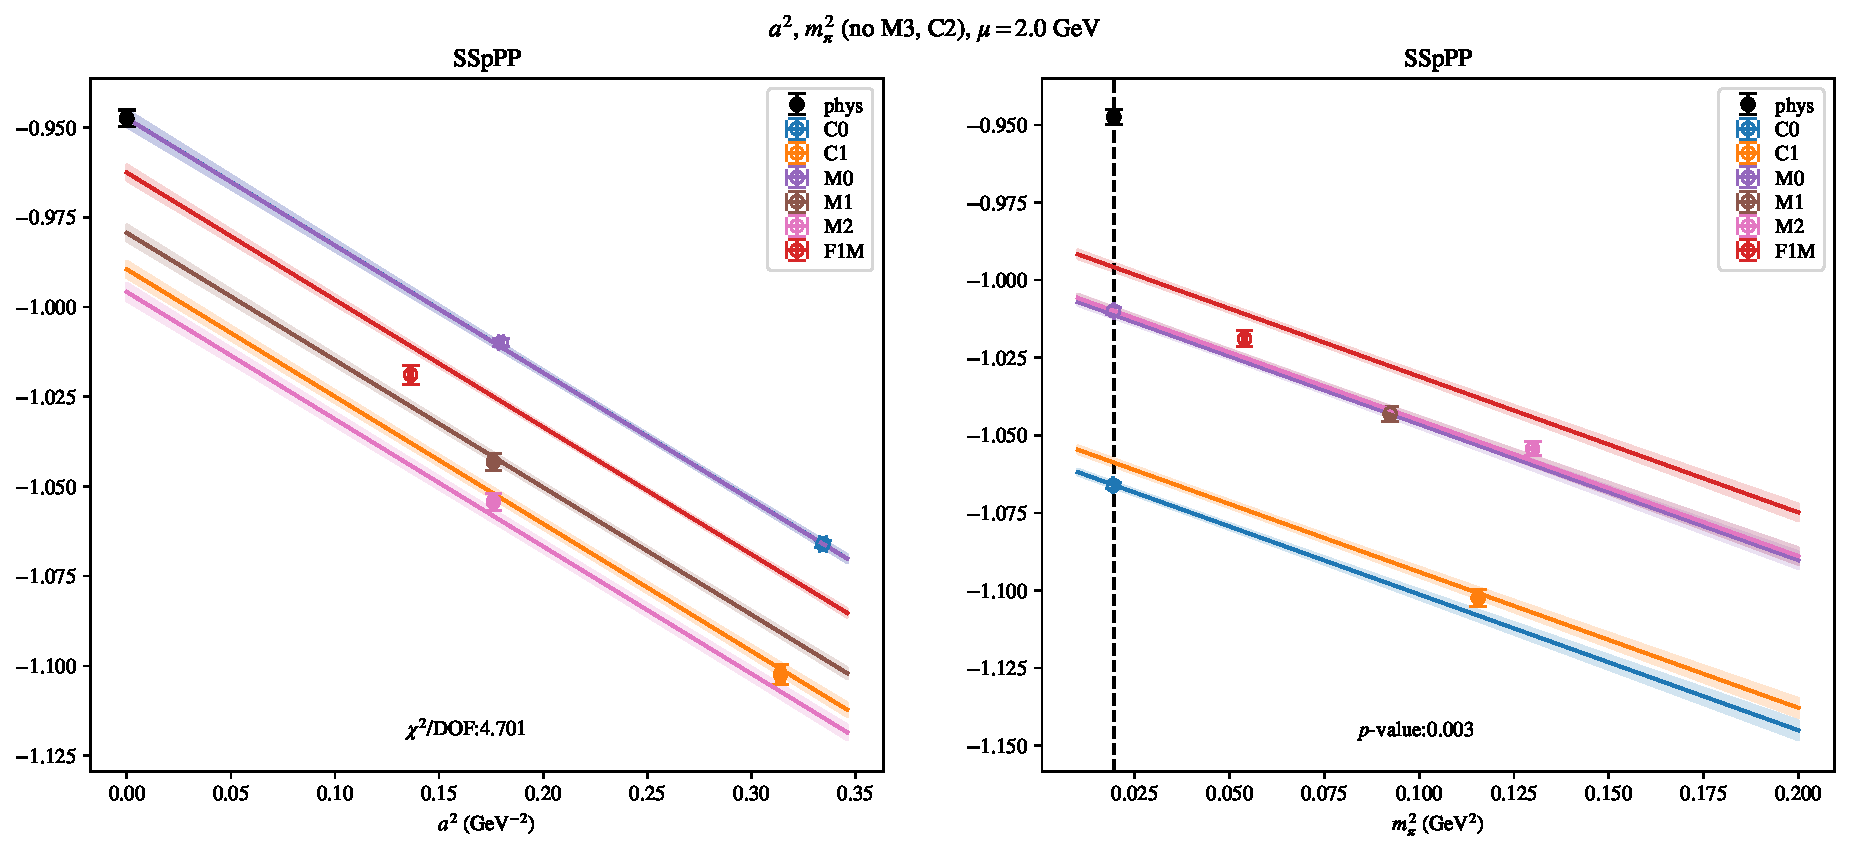
\includepdf[link, pages=-]{VVmAA/SUSY/a2m2mcut_20.pdf}
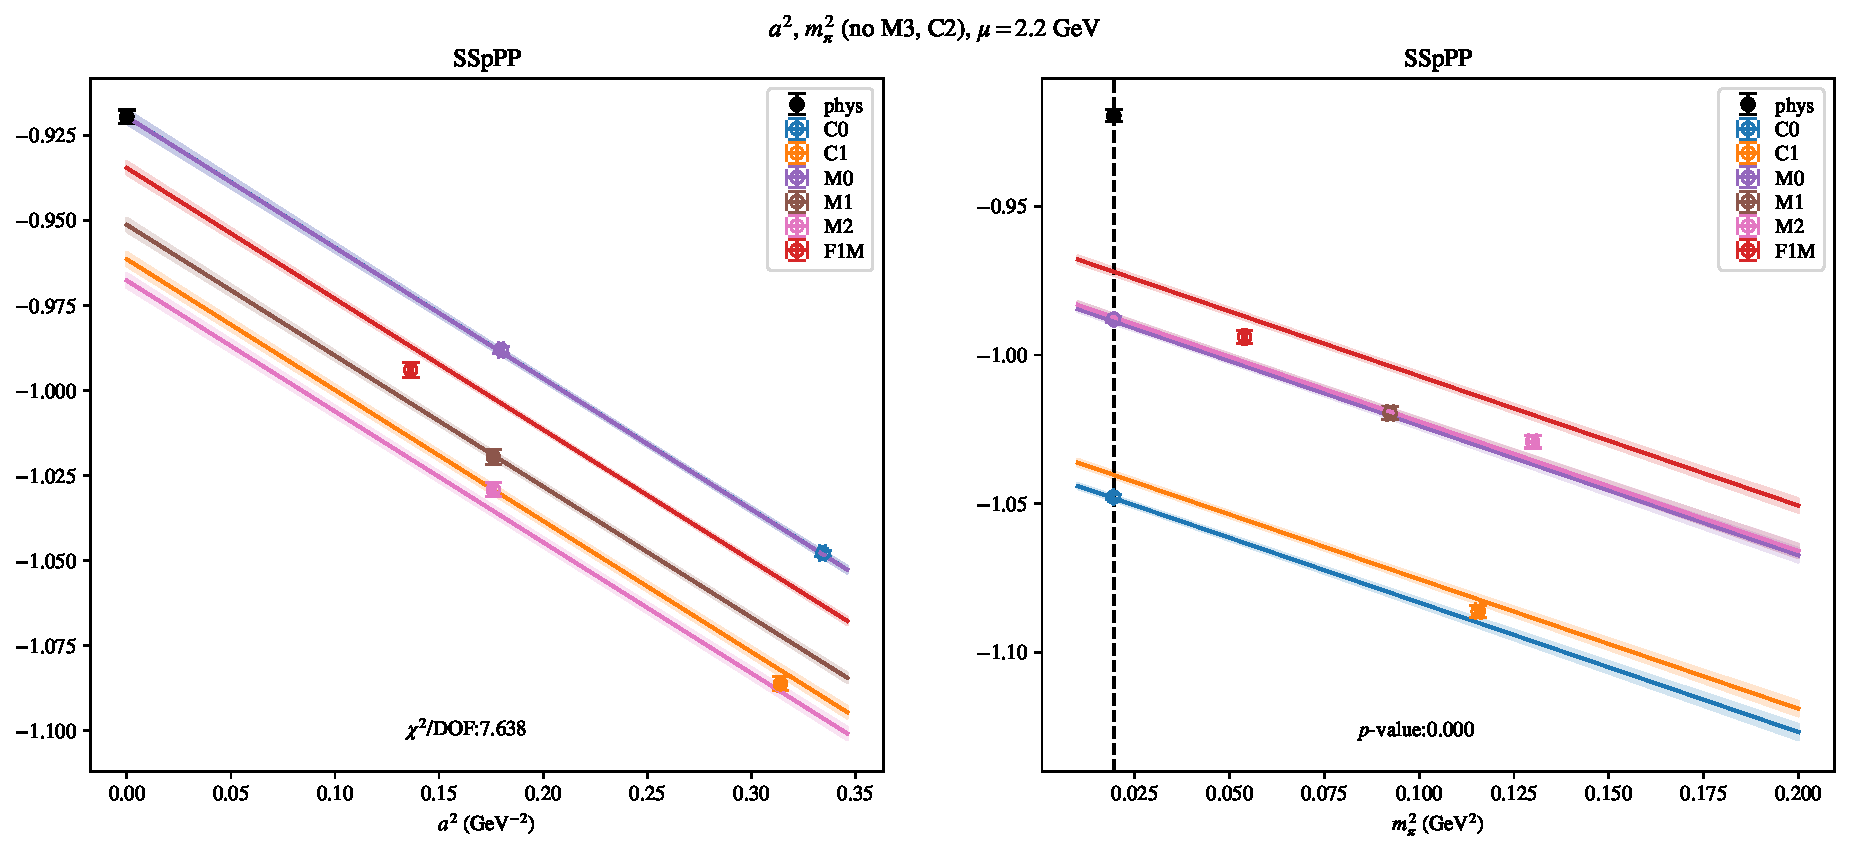
\includepdf[link, pages=-]{VVmAA/SUSY/a2m2mcut_22.pdf}
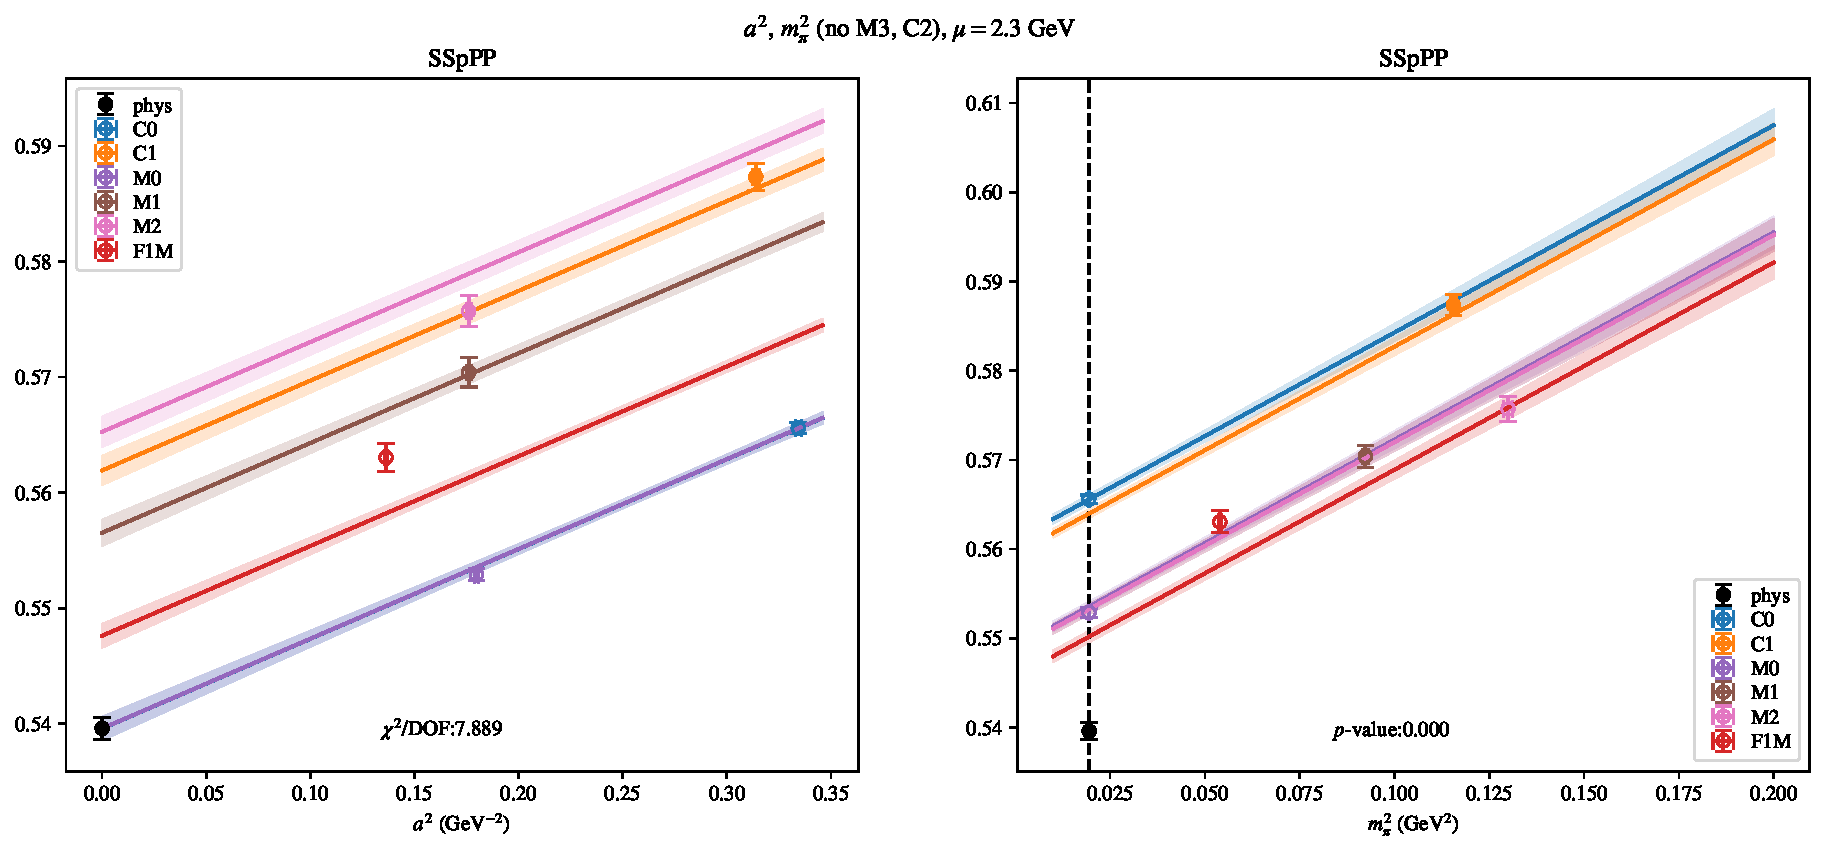
\includepdf[link, pages=-]{VVmAA/SUSY/a2m2mcut_23.pdf}
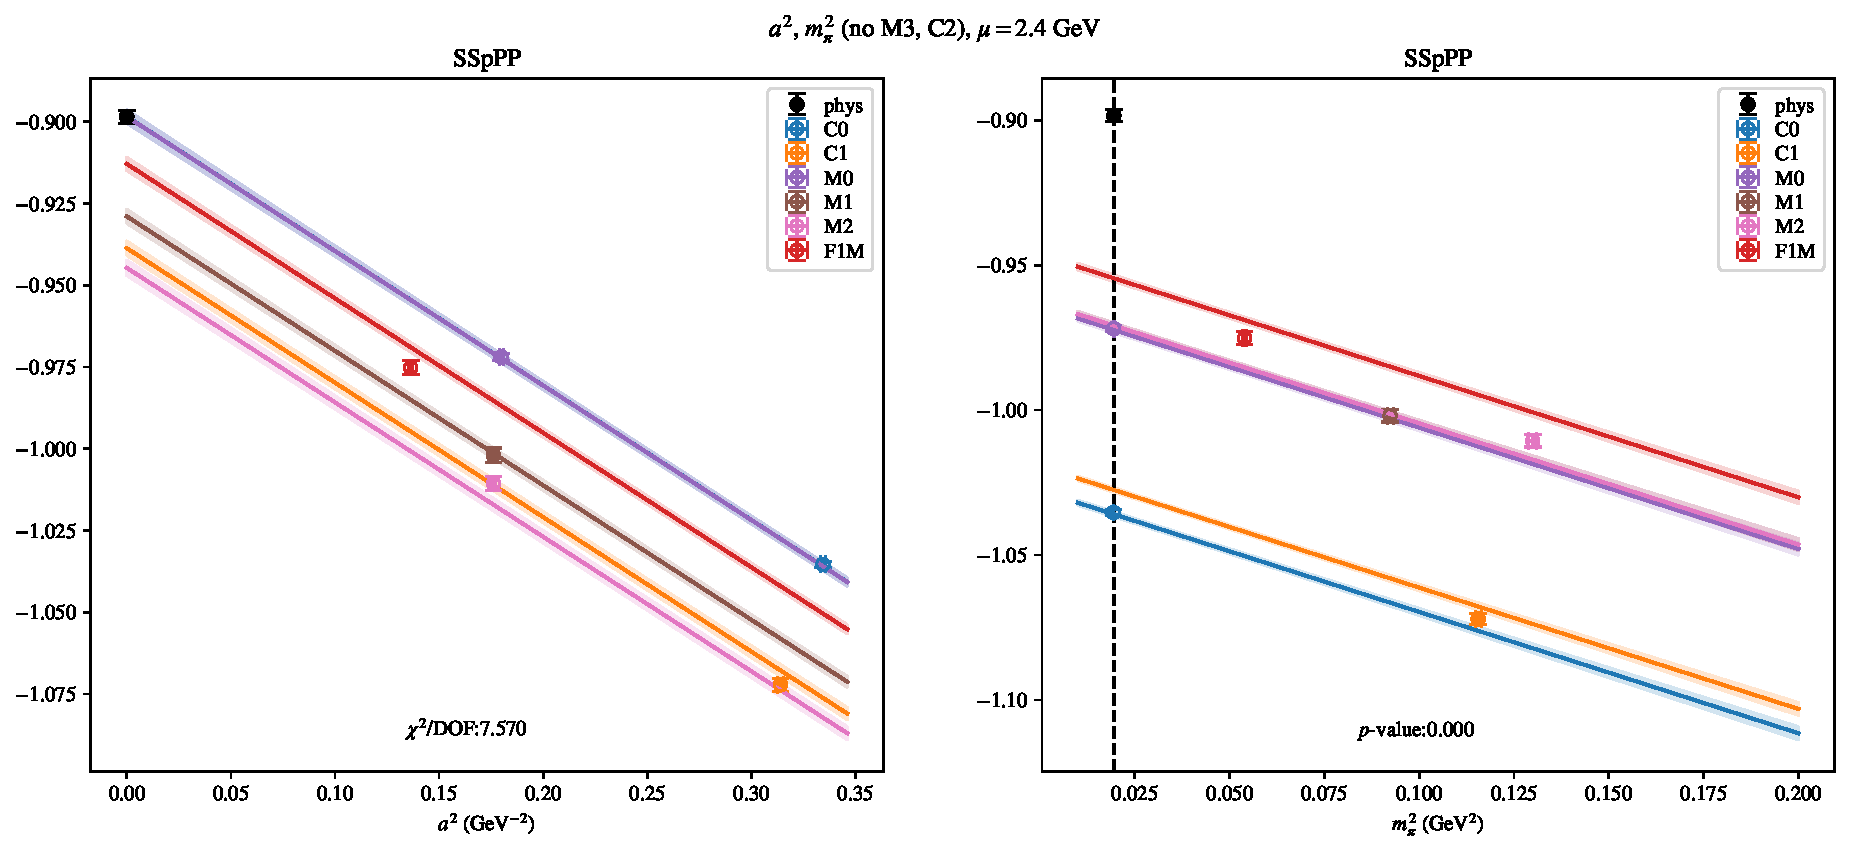
\includepdf[link, pages=-]{VVmAA/SUSY/a2m2mcut_24.pdf}
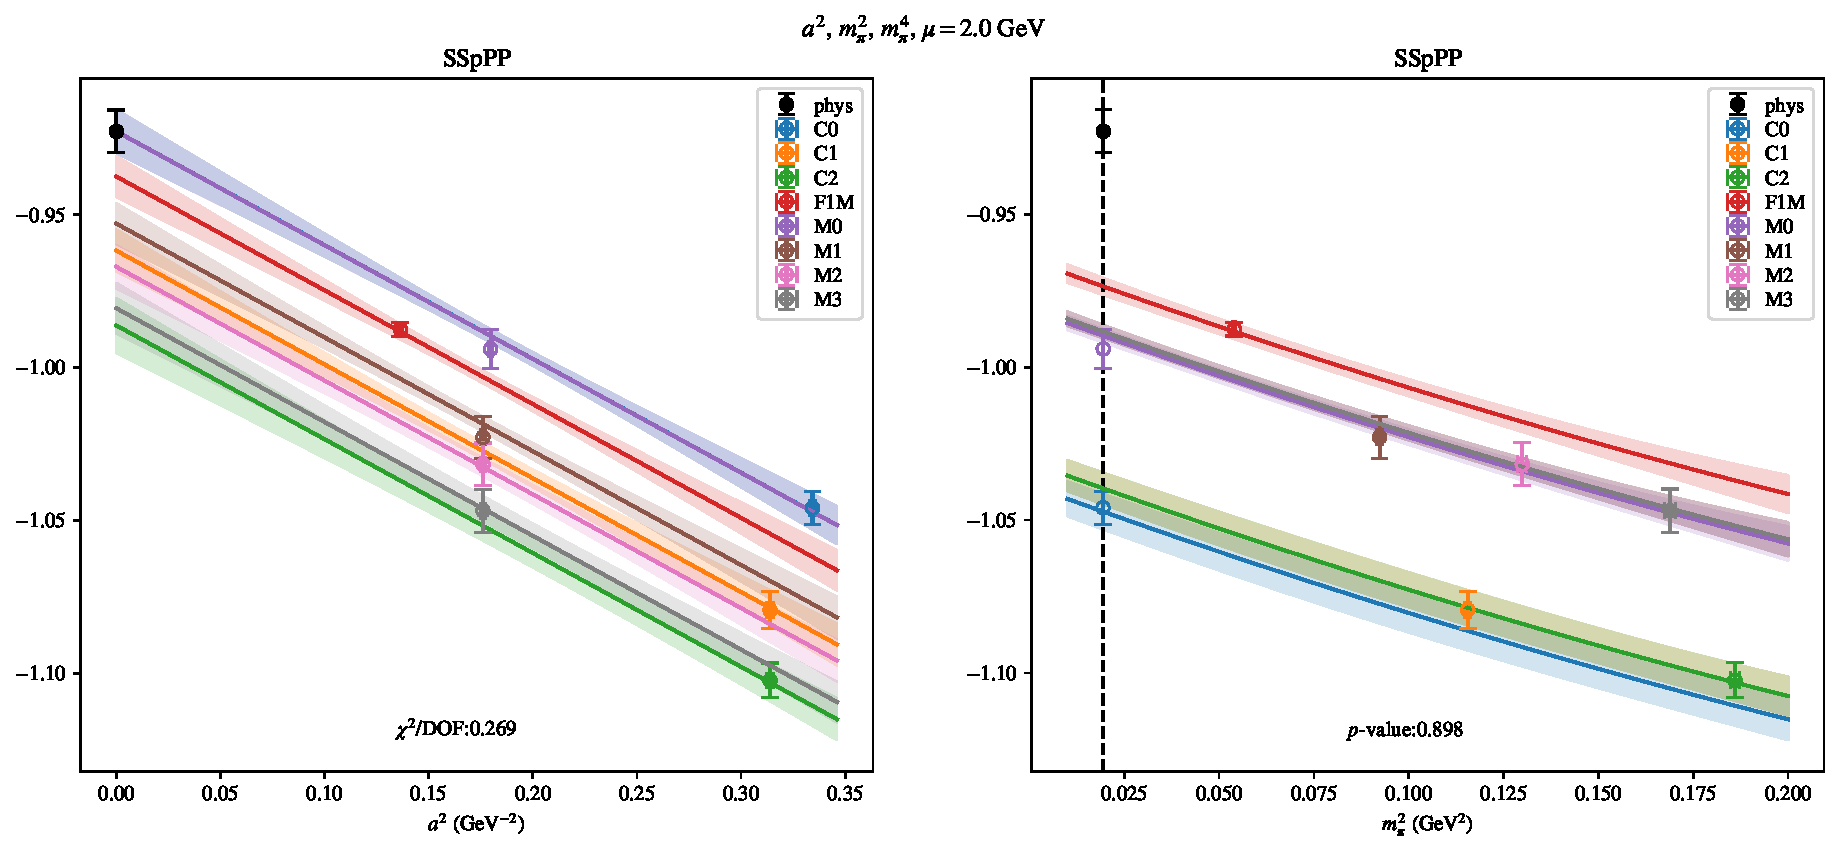
\includepdf[link, pages=-]{VVmAA/SUSY/a2m2m4_20.pdf}
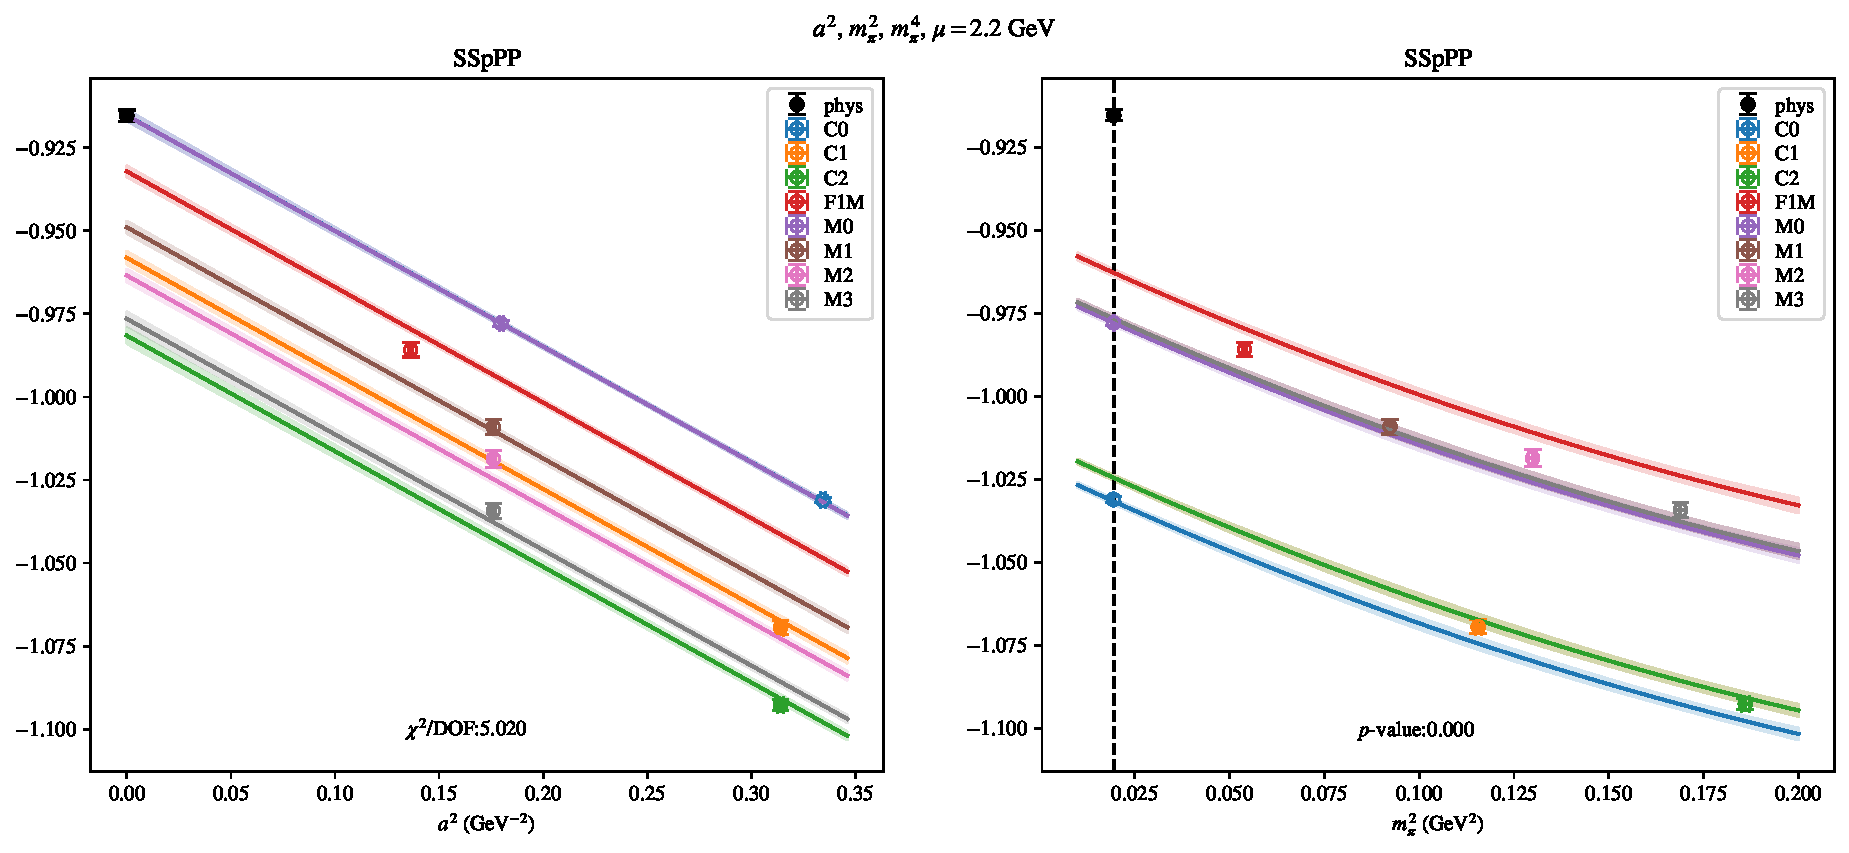
\includepdf[link, pages=-]{VVmAA/SUSY/a2m2m4_22.pdf}
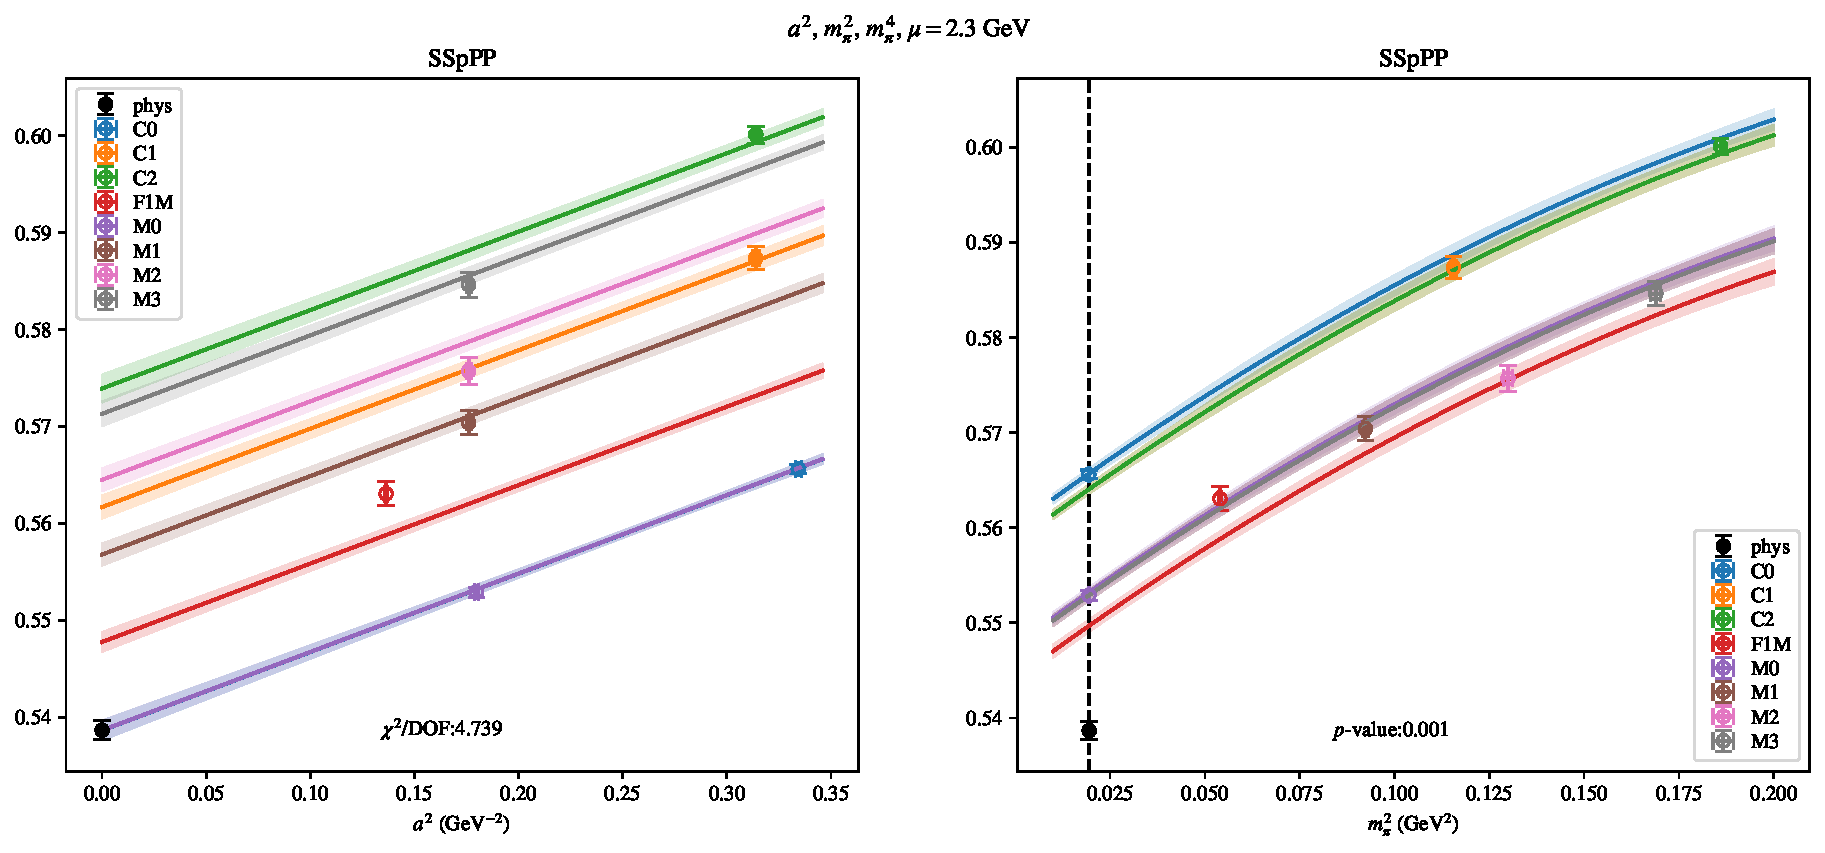
\includepdf[link, pages=-]{VVmAA/SUSY/a2m2m4_23.pdf}
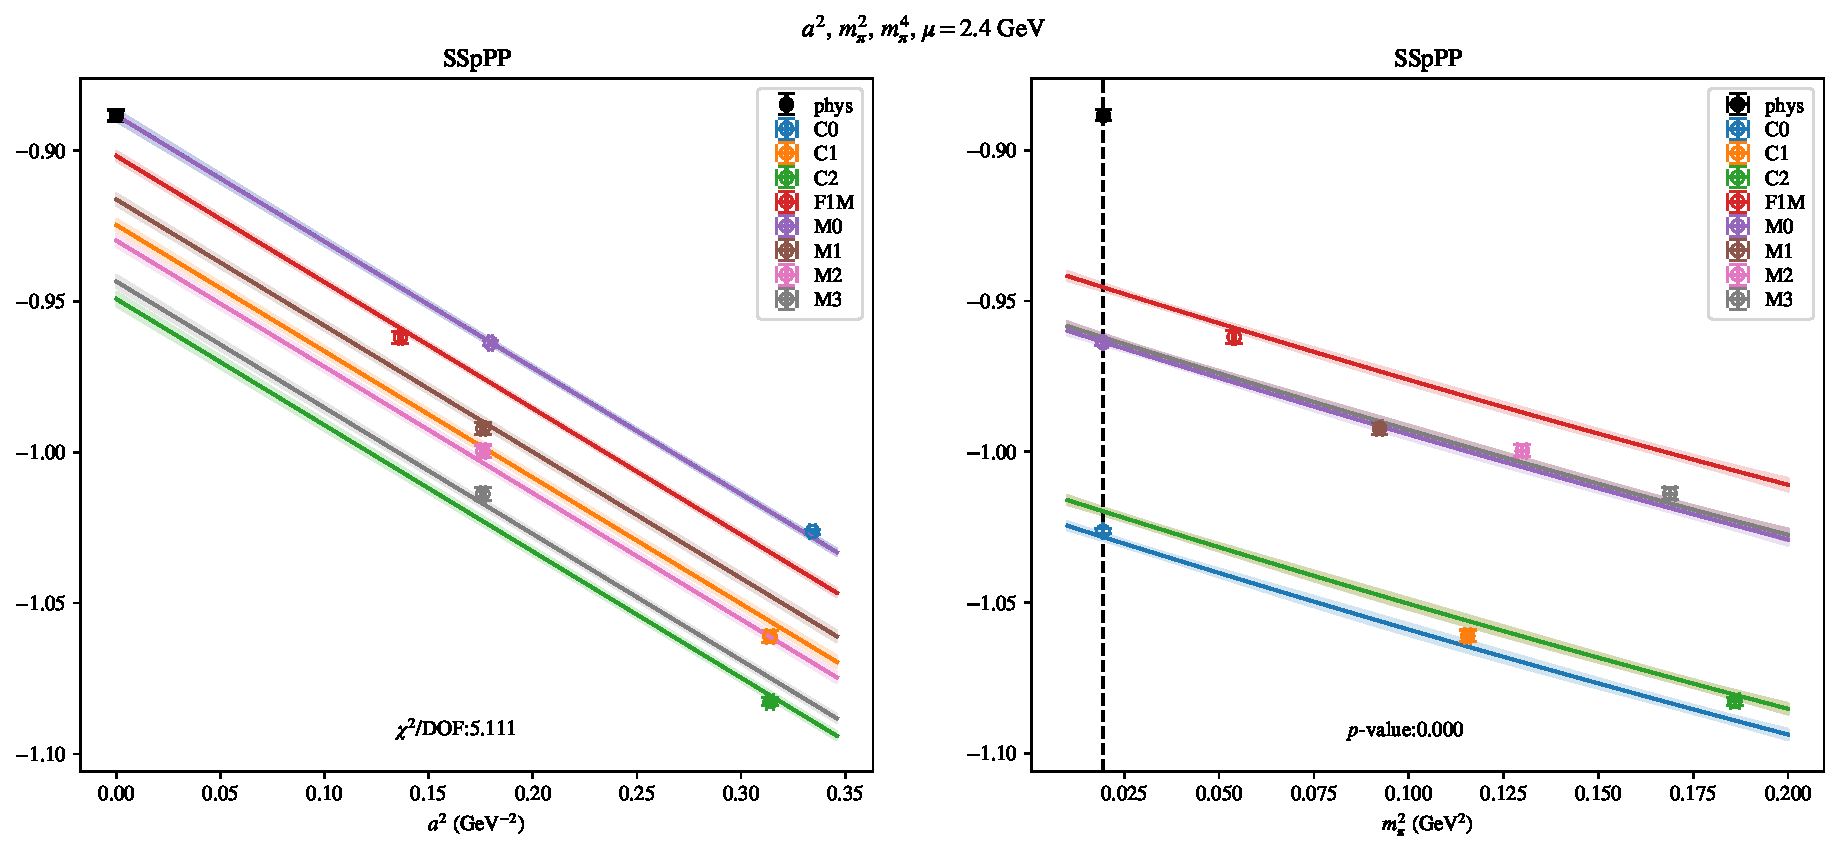
\includepdf[link, pages=-]{VVmAA/SUSY/a2m2m4_24.pdf}
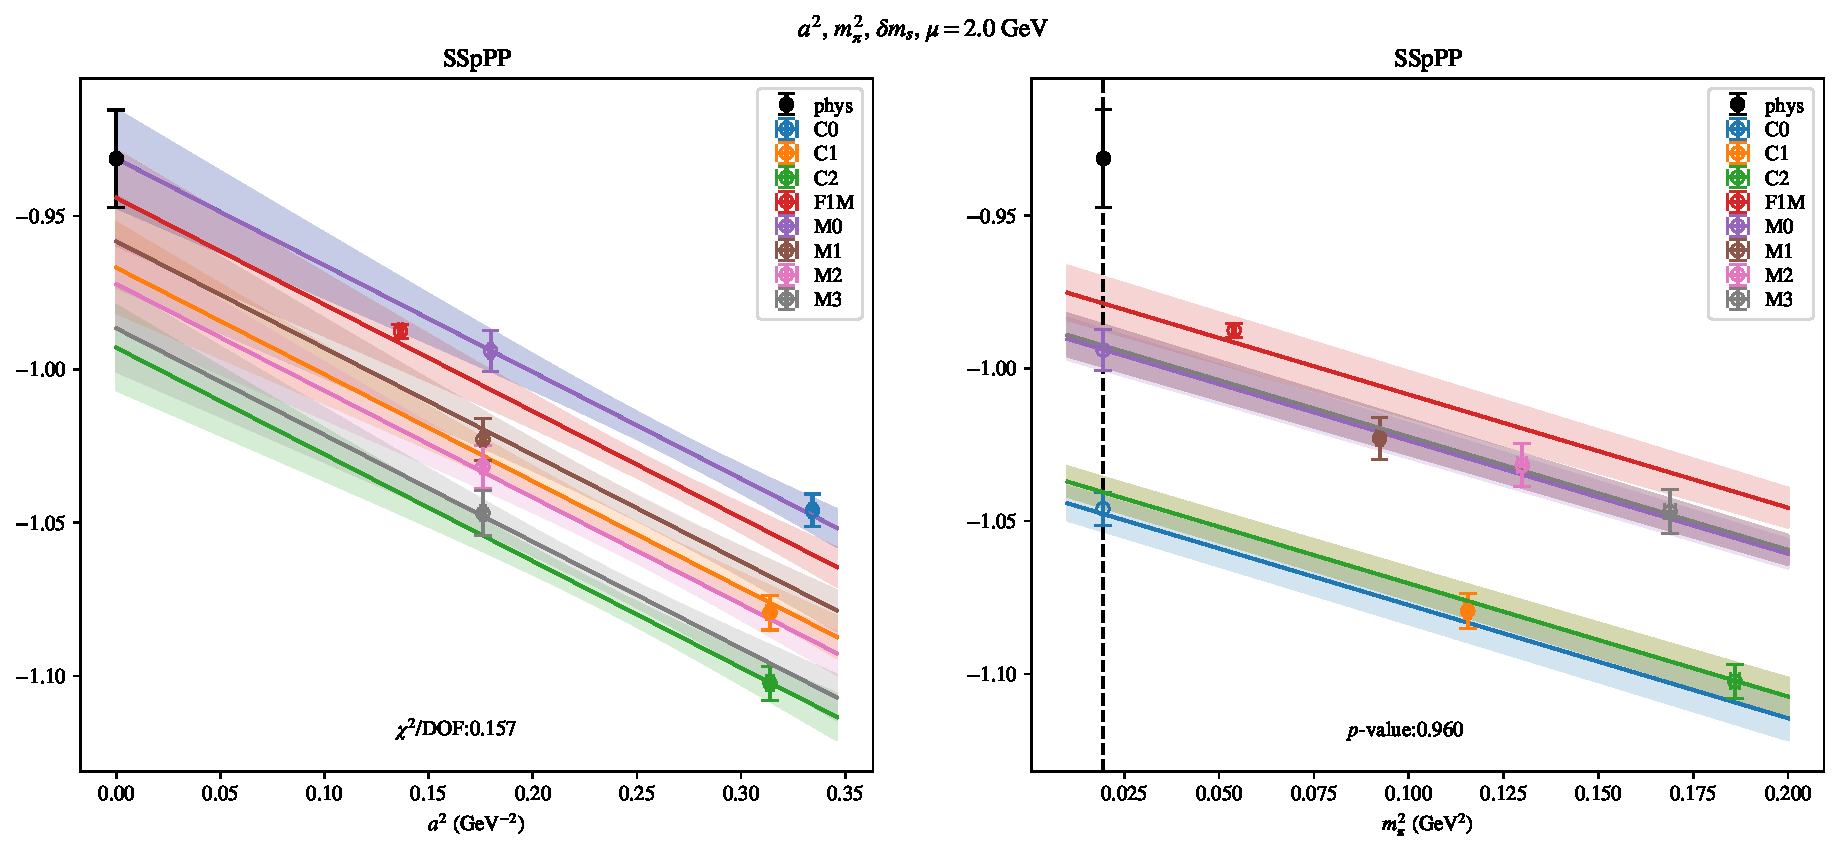
\includepdf[link, pages=-]{VVmAA/SUSY/a2m2delm_20.pdf}
\includepdf[link, pages=-]{VVmAA/SUSY/a2m2delm_22.pdf}
\includepdf[link, pages=-]{VVmAA/SUSY/a2m2delm_23.pdf}
\includepdf[link, pages=-]{VVmAA/SUSY/a2m2delm_24.pdf}
\clearpage
\section{$\mathcal{B}_3$}
\begin{table}[h!]
\begin{center}
\begin{tabular}{|c|c|c|c|c|c|c|}
\hline
$\mu$ (GeV) & $a^2$, $m_\pi^2$& $a^2$, $m_\pi^2$ (no C)& $a^2$, $a^4$, $m_\pi^2$& $a^2$, $m_\pi^2$ (no M3, C2)& $a^2$, $m_\pi^2$, $m_\pi^4$& $a^2$, $m_\pi^2$, $\delta m_s$\\
\hline
2.0& \hyperlink{SSmPP/SUSY/a2m2_20.pdf.1}{\textbf{0.28191(73)}: 0.96 (0.441)} & \hyperlink{SSmPP/SUSY/a2m2noC_20.pdf.1}{\textbf{0.2816(36)}: 1.31 (0.27)} & \hyperlink{SSmPP/SUSY/a2a4m2_20.pdf.1}{\textbf{0.2815(57)}: 1.199 (0.309)} & \hyperlink{SSmPP/SUSY/a2m2mcut_20.pdf.1}{\textbf{0.28165(75)}: 0.72 (0.54)} & \hyperlink{SSmPP/SUSY/a2m2m4_20.pdf.1}{\textbf{0.28149(78)}: 0.578 (0.678)} & \hyperlink{SSmPP/SUSY/a2m2delm_20.pdf.1}{\textbf{0.28195(85)}: 1.195 (0.311)}\\
2.2& \hyperlink{SSmPP/SUSY/a2m2_22.pdf.1}{\textbf{0.27370(69)}: 1.946 (0.083)} & \hyperlink{SSmPP/SUSY/a2m2noC_22.pdf.1}{\textbf{0.2766(32)}: 1.566 (0.209)} & \hyperlink{SSmPP/SUSY/a2a4m2_22.pdf.1}{\textbf{0.2757(53)}: 2.387 (0.049)} & \hyperlink{SSmPP/SUSY/a2m2mcut_22.pdf.1}{\textbf{0.27348(71)}: 1.464 (0.222)} & \hyperlink{SSmPP/SUSY/a2m2m4_22.pdf.1}{\textbf{0.27314(74)}: 0.952 (0.433)} & \hyperlink{SSmPP/SUSY/a2m2delm_22.pdf.1}{\textbf{0.27351(81)}: 2.32 (0.054)}\\
2.3& \hyperlink{SSmPP/SUSY/a2m2_23.pdf.1}{\textbf{0.26979(68)}: 2.639 (0.022)} & \hyperlink{SSmPP/SUSY/a2m2noC_23.pdf.1}{\textbf{0.2740(30)}: 1.916 (0.147)} & \hyperlink{SSmPP/SUSY/a2a4m2_23.pdf.1}{\textbf{0.2730(52)}: 3.173 (0.013)} & \hyperlink{SSmPP/SUSY/a2m2mcut_23.pdf.1}{\textbf{0.26961(71)}: 2.34 (0.071)} & \hyperlink{SSmPP/SUSY/a2m2m4_23.pdf.1}{\textbf{0.26920(73)}: 1.583 (0.176)} & \hyperlink{SSmPP/SUSY/a2m2delm_23.pdf.1}{\textbf{0.26950(79)}: 2.991 (0.018)}\\
2.4& \hyperlink{SSmPP/SUSY/a2m2_24.pdf.1}{\textbf{0.26647(67)}: 3.264 (0.006)} & \hyperlink{SSmPP/SUSY/a2m2noC_24.pdf.1}{\textbf{0.2712(30)}: 2.247 (0.106)} & \hyperlink{SSmPP/SUSY/a2a4m2_24.pdf.1}{\textbf{0.2695(52)}: 3.96 (0.003)} & \hyperlink{SSmPP/SUSY/a2m2mcut_24.pdf.1}{\textbf{0.26635(71)}: 3.163 (0.023)} & \hyperlink{SSmPP/SUSY/a2m2m4_24.pdf.1}{\textbf{0.26587(74)}: 2.359 (0.051)} & \hyperlink{SSmPP/SUSY/a2m2delm_24.pdf.1}{\textbf{0.26616(78)}: 3.681 (0.005)}\\
\hline
\end{tabular}
\caption{Physical point value from chiral and continuum extrapolation at renormalisation scale $\mu$. Entries are \textbf{value(error)}: $\chi^2/\text{DOF}$ ($p$-value).}
\end{center}
\end{table}
\begin{table}[h!]
\begin{center}
\begin{tabular}{|c c|c|c|c|c|c|c|}
\hline
$\mu$ (GeV) &  & $a^2$, $m_\pi^2$& $a^2$, $m_\pi^2$ (no C)& $a^2$, $a^4$, $m_\pi^2$& $a^2$, $m_\pi^2$ (no M3, C2)& $a^2$, $m_\pi^2$, $m_\pi^4$& $a^2$, $m_\pi^2$, $\delta m_s$\\
\hline
\multirow{2}{0.5in}{2.0} & $\alpha$ & 0.636(12)& 0.641(82)& 0.64(19)& 0.639(12)& 0.642(12)& 0.635(13)\\
 & $\beta$ & 0.00816(46)& 0.00827(87)& 0.00817(51)& 0.00885(63)& 0.0105(13)& 0.00816(46)\\
\hline
\multirow{2}{0.5in}{2.2} & $\alpha$ & 0.742(12)& 0.674(76)& 0.67(19)& 0.745(12)& 0.750(12)& 0.745(14)\\
 & $\beta$ & 0.00806(30)& 0.00770(61)& 0.00802(33)& 0.00879(46)& 0.0108(11)& 0.00809(30)\\
\hline
\multirow{2}{0.5in}{2.3} & $\alpha$ & 0.799(12)& 0.698(74)& 0.68(19)& 0.801(13)& 0.808(13)& 0.803(14)\\
 & $\beta$ & 0.00817(27)& 0.00765(52)& 0.00810(30)& 0.00887(43)& 0.0109(10)& 0.00822(27)\\
\hline
\multirow{2}{0.5in}{2.4} & $\alpha$ & 0.850(12)& 0.737(73)& 0.73(19)& 0.851(13)& 0.859(13)& 0.855(14)\\
 & $\beta$ & 0.00824(26)& 0.00762(45)& 0.00817(28)& 0.00888(40)& 0.0109(10)& 0.00830(26)\\
\hline
\end{tabular}
\caption{Fit values of coefficients in $Q = Q_{phys} + \mathbf{\alpha} a^2 + \mathbf{\beta}\left(\frac{m_\pi^2}{f_\pi^2}-\frac{m_{\pi,PDG}^2}{f_\pi^2}\right) + \ldots$.}
\end{center}
\end{table}
\includepdf[link, pages=-]{SSmPP/SUSY/a2m2_20.pdf}
\includepdf[link, pages=-]{SSmPP/SUSY/a2m2_22.pdf}
\includepdf[link, pages=-]{SSmPP/SUSY/a2m2_23.pdf}
\includepdf[link, pages=-]{SSmPP/SUSY/a2m2_24.pdf}
\includepdf[link, pages=-]{SSmPP/SUSY/a2m2noC_20.pdf}
\includepdf[link, pages=-]{SSmPP/SUSY/a2m2noC_22.pdf}
\includepdf[link, pages=-]{SSmPP/SUSY/a2m2noC_23.pdf}
\includepdf[link, pages=-]{SSmPP/SUSY/a2m2noC_24.pdf}
\includepdf[link, pages=-]{SSmPP/SUSY/a2a4m2_20.pdf}
\includepdf[link, pages=-]{SSmPP/SUSY/a2a4m2_22.pdf}
\includepdf[link, pages=-]{SSmPP/SUSY/a2a4m2_23.pdf}
\includepdf[link, pages=-]{SSmPP/SUSY/a2a4m2_24.pdf}
\includepdf[link, pages=-]{SSmPP/SUSY/a2m2mcut_20.pdf}
\includepdf[link, pages=-]{SSmPP/SUSY/a2m2mcut_22.pdf}
\includepdf[link, pages=-]{SSmPP/SUSY/a2m2mcut_23.pdf}
\includepdf[link, pages=-]{SSmPP/SUSY/a2m2mcut_24.pdf}
\includepdf[link, pages=-]{SSmPP/SUSY/a2m2m4_20.pdf}
\includepdf[link, pages=-]{SSmPP/SUSY/a2m2m4_22.pdf}
\includepdf[link, pages=-]{SSmPP/SUSY/a2m2m4_23.pdf}
\includepdf[link, pages=-]{SSmPP/SUSY/a2m2m4_24.pdf}
\includepdf[link, pages=-]{SSmPP/SUSY/a2m2delm_20.pdf}
\includepdf[link, pages=-]{SSmPP/SUSY/a2m2delm_22.pdf}
\includepdf[link, pages=-]{SSmPP/SUSY/a2m2delm_23.pdf}
\includepdf[link, pages=-]{SSmPP/SUSY/a2m2delm_24.pdf}
\clearpage
\section{$\mathcal{B}_4$}
\begin{table}[h!]
\begin{center}
\begin{tabular}{|c|c|c|c|c|c|c|}
\hline
$\mu$ (GeV) & $a^2$, $m_\pi^2$& $a^2$, $m_\pi^2$ (no C)& $a^2$, $a^4$, $m_\pi^2$& $a^2$, $m_\pi^2$ (no M3, C2)& $a^2$, $m_\pi^2$, $m_\pi^4$& $a^2$, $m_\pi^2$, $\delta m_s$\\
\hline
2.0& \hyperlink{SSpPP/SUSY/a2m2_20.pdf.1}{\textbf{1.7996(29)}: 19.012 (0.0)} & \hyperlink{SSpPP/SUSY/a2m2noC_20.pdf.1}{\textbf{1.672(15)}: 0.134 (0.874)} & \hyperlink{SSpPP/SUSY/a2a4m2_20.pdf.1}{\textbf{1.596(21)}: 1.117 (0.346)} & \hyperlink{SSpPP/SUSY/a2m2mcut_20.pdf.1}{\textbf{1.8014(29)}: 27.796 (0.0)} & \hyperlink{SSpPP/SUSY/a2m2m4_20.pdf.1}{\textbf{1.8073(30)}: 13.852 (0.0)} & \hyperlink{SSpPP/SUSY/a2m2delm_20.pdf.1}{\textbf{1.8138(32)}: 0.249 (0.91)}\\
2.2& \hyperlink{SSpPP/SUSY/a2m2_22.pdf.1}{\textbf{1.8059(28)}: 15.663 (0.0)} & \hyperlink{SSpPP/SUSY/a2m2noC_22.pdf.1}{\textbf{1.696(13)}: 0.638 (0.528)} & \hyperlink{SSpPP/SUSY/a2a4m2_22.pdf.1}{\textbf{1.631(21)}: 1.406 (0.229)} & \hyperlink{SSpPP/SUSY/a2m2mcut_22.pdf.1}{\textbf{1.8070(28)}: 23.604 (0.0)} & \hyperlink{SSpPP/SUSY/a2m2m4_22.pdf.1}{\textbf{1.8114(29)}: 13.666 (0.0)} & \hyperlink{SSpPP/SUSY/a2m2delm_22.pdf.1}{\textbf{1.8183(32)}: 0.828 (0.507)}\\
2.3& \hyperlink{SSpPP/SUSY/a2m2_23.pdf.1}{\textbf{1.8081(28)}: 15.164 (0.0)} & \hyperlink{SSpPP/SUSY/a2m2noC_23.pdf.1}{\textbf{1.702(13)}: 0.824 (0.439)} & \hyperlink{SSpPP/SUSY/a2a4m2_23.pdf.1}{\textbf{1.636(20)}: 1.212 (0.303)} & \hyperlink{SSpPP/SUSY/a2m2mcut_23.pdf.1}{\textbf{1.8092(28)}: 23.139 (0.0)} & \hyperlink{SSpPP/SUSY/a2m2m4_23.pdf.1}{\textbf{1.8133(29)}: 13.626 (0.0)} & \hyperlink{SSpPP/SUSY/a2m2delm_23.pdf.1}{\textbf{1.8197(32)}: 1.089 (0.36)}\\
2.4& \hyperlink{SSpPP/SUSY/a2m2_24.pdf.1}{\textbf{1.8096(27)}: 14.186 (0.0)} & \hyperlink{SSpPP/SUSY/a2m2noC_24.pdf.1}{\textbf{1.707(13)}: 0.955 (0.385)} & \hyperlink{SSpPP/SUSY/a2a4m2_24.pdf.1}{\textbf{1.645(20)}: 1.418 (0.225)} & \hyperlink{SSpPP/SUSY/a2m2mcut_24.pdf.1}{\textbf{1.8103(28)}: 21.876 (0.0)} & \hyperlink{SSpPP/SUSY/a2m2m4_24.pdf.1}{\textbf{1.8143(28)}: 13.497 (0.0)} & \hyperlink{SSpPP/SUSY/a2m2delm_24.pdf.1}{\textbf{1.8203(31)}: 1.208 (0.305)}\\
\hline
\end{tabular}
\caption{Physical point value from chiral and continuum extrapolation at renormalisation scale $\mu$. Entries are \textbf{value(error)}: $\chi^2/\text{DOF}$ ($p$-value).}
\end{center}
\end{table}
\begin{table}[h!]
\begin{center}
\begin{tabular}{|c c|c|c|c|c|c|c|}
\hline
$\mu$ (GeV) &  & $a^2$, $m_\pi^2$& $a^2$, $m_\pi^2$ (no C)& $a^2$, $a^4$, $m_\pi^2$& $a^2$, $m_\pi^2$ (no M3, C2)& $a^2$, $m_\pi^2$, $m_\pi^4$& $a^2$, $m_\pi^2$, $\delta m_s$\\
\hline
\multirow{2}{0.5in}{2.0} & $\alpha$ & 0.0715(63)& 0.516(57)& 1.21(13)& 0.0683(64)& 0.0567(64)& 0.0441(68)\\
 & $\beta$ & -0.0005(31)& 0.00017(64)& -0.0005(35)& -0.0016(44)& -0.0070(94)& -0.0004(31)\\
\hline
\multirow{2}{0.5in}{2.2} & $\alpha$ & 0.0755(61)& 0.454(49)& 1.04(12)& 0.0739(61)& 0.0654(61)& 0.0519(67)\\
 & $\beta$ & -0.0005(19)& -0.0003(46)& -0.0009(22)& -0.0011(31)& -0.0044(77)& -0.0007(19)\\
\hline
\multirow{2}{0.5in}{2.3} & $\alpha$ & 0.0769(60)& 0.443(49)& 1.02(12)& 0.0754(60)& 0.0674(61)& 0.0550(66)\\
 & $\beta$ & -0.0004(18)& -0.0003(38)& -0.0007(21)& -0.0009(29)& -0.0039(73)& -0.0006(17)\\
\hline
\multirow{2}{0.5in}{2.4} & $\alpha$ & 0.0786(59)& 0.431(48)& 0.98(12)& 0.0777(60)& 0.0700(61)& 0.0584(65)\\
 & $\beta$ & -0.0003(15)& -0.0003(33)& -0.0007(18)& -0.0008(26)& -0.0033(70)& -0.0005(15)\\
\hline
\end{tabular}
\caption{Fit values of coefficients in $Q = Q_{phys} + \mathbf{\alpha} a^2 + \mathbf{\beta}\left(\frac{m_\pi^2}{f_\pi^2}-\frac{m_{\pi,PDG}^2}{f_\pi^2}\right) + \ldots$.}
\end{center}
\end{table}
\includepdf[link, pages=-]{SSpPP/SUSY/a2m2_20.pdf}
\includepdf[link, pages=-]{SSpPP/SUSY/a2m2_22.pdf}
\includepdf[link, pages=-]{SSpPP/SUSY/a2m2_23.pdf}
\includepdf[link, pages=-]{SSpPP/SUSY/a2m2_24.pdf}
\includepdf[link, pages=-]{SSpPP/SUSY/a2m2noC_20.pdf}
\includepdf[link, pages=-]{SSpPP/SUSY/a2m2noC_22.pdf}
\includepdf[link, pages=-]{SSpPP/SUSY/a2m2noC_23.pdf}
\includepdf[link, pages=-]{SSpPP/SUSY/a2m2noC_24.pdf}
\includepdf[link, pages=-]{SSpPP/SUSY/a2a4m2_20.pdf}
\includepdf[link, pages=-]{SSpPP/SUSY/a2a4m2_22.pdf}
\includepdf[link, pages=-]{SSpPP/SUSY/a2a4m2_23.pdf}
\includepdf[link, pages=-]{SSpPP/SUSY/a2a4m2_24.pdf}
\includepdf[link, pages=-]{SSpPP/SUSY/a2m2mcut_20.pdf}
\includepdf[link, pages=-]{SSpPP/SUSY/a2m2mcut_22.pdf}
\includepdf[link, pages=-]{SSpPP/SUSY/a2m2mcut_23.pdf}
\includepdf[link, pages=-]{SSpPP/SUSY/a2m2mcut_24.pdf}
\includepdf[link, pages=-]{SSpPP/SUSY/a2m2m4_20.pdf}
\includepdf[link, pages=-]{SSpPP/SUSY/a2m2m4_22.pdf}
\includepdf[link, pages=-]{SSpPP/SUSY/a2m2m4_23.pdf}
\includepdf[link, pages=-]{SSpPP/SUSY/a2m2m4_24.pdf}
\includepdf[link, pages=-]{SSpPP/SUSY/a2m2delm_20.pdf}
\includepdf[link, pages=-]{SSpPP/SUSY/a2m2delm_22.pdf}
\includepdf[link, pages=-]{SSpPP/SUSY/a2m2delm_23.pdf}
\includepdf[link, pages=-]{SSpPP/SUSY/a2m2delm_24.pdf}
\clearpage
\section{$\mathcal{B}_5$}
\begin{table}[h!]
\begin{center}
\begin{tabular}{|c|c|c|c|c|c|c|}
\hline
$\mu$ (GeV) & $a^2$, $m_\pi^2$& $a^2$, $m_\pi^2$ (no C)& $a^2$, $a^4$, $m_\pi^2$& $a^2$, $m_\pi^2$ (no M3, C2)& $a^2$, $m_\pi^2$, $m_\pi^4$& $a^2$, $m_\pi^2$, $\delta m_s$\\
\hline
2.0& \hyperlink{TT/SUSY/a2m2_20.pdf.1}{\textbf{0.49589(82)}: 11.93 (0.0)} & \hyperlink{TT/SUSY/a2m2noC_20.pdf.1}{\textbf{0.4610(51)}: 0.371 (0.69)} & \hyperlink{TT/SUSY/a2a4m2_20.pdf.1}{\textbf{0.4417(72)}: 1.064 (0.372)} & \hyperlink{TT/SUSY/a2m2mcut_20.pdf.1}{\textbf{0.49617(82)}: 17.434 (0.0)} & \hyperlink{TT/SUSY/a2m2m4_20.pdf.1}{\textbf{0.49712(82)}: 9.382 (0.0)} & \hyperlink{TT/SUSY/a2m2delm_20.pdf.1}{\textbf{0.49829(90)}: 0.463 (0.763)}\\
2.2& \hyperlink{TT/SUSY/a2m2_22.pdf.1}{\textbf{0.50301(78)}: 9.9 (0.0)} & \hyperlink{TT/SUSY/a2m2noC_22.pdf.1}{\textbf{0.4736(46)}: 1.21 (0.298)} & \hyperlink{TT/SUSY/a2a4m2_22.pdf.1}{\textbf{0.4566(72)}: 1.275 (0.277)} & \hyperlink{TT/SUSY/a2m2mcut_22.pdf.1}{\textbf{0.50327(76)}: 14.22 (0.0)} & \hyperlink{TT/SUSY/a2m2m4_22.pdf.1}{\textbf{0.50395(76)}: 8.022 (0.0)} & \hyperlink{TT/SUSY/a2m2delm_22.pdf.1}{\textbf{0.50495(86)}: 1.401 (0.231)}\\
2.3& \hyperlink{TT/SUSY/a2m2_23.pdf.1}{\textbf{0.50607(77)}: 10.382 (0.0)} & \hyperlink{TT/SUSY/a2m2noC_23.pdf.1}{\textbf{0.4771(45)}: 1.585 (0.205)} & \hyperlink{TT/SUSY/a2a4m2_23.pdf.1}{\textbf{0.4592(70)}: 1.265 (0.281)} & \hyperlink{TT/SUSY/a2m2mcut_23.pdf.1}{\textbf{0.50636(75)}: 15.161 (0.0)} & \hyperlink{TT/SUSY/a2m2m4_23.pdf.1}{\textbf{0.50701(76)}: 8.679 (0.0)} & \hyperlink{TT/SUSY/a2m2delm_23.pdf.1}{\textbf{0.50789(86)}: 1.918 (0.104)}\\
2.4& \hyperlink{TT/SUSY/a2m2_24.pdf.1}{\textbf{0.50832(77)}: 9.612 (0.0)} & \hyperlink{TT/SUSY/a2m2noC_24.pdf.1}{\textbf{0.4807(44)}: 1.789 (0.167)} & \hyperlink{TT/SUSY/a2a4m2_24.pdf.1}{\textbf{0.4646(70)}: 1.51 (0.196)} & \hyperlink{TT/SUSY/a2m2mcut_24.pdf.1}{\textbf{0.50858(75)}: 13.988 (0.0)} & \hyperlink{TT/SUSY/a2m2m4_24.pdf.1}{\textbf{0.50925(76)}: 8.159 (0.0)} & \hyperlink{TT/SUSY/a2m2delm_24.pdf.1}{\textbf{0.51002(86)}: 1.961 (0.097)}\\
\hline
\end{tabular}
\caption{Physical point value from chiral and continuum extrapolation at renormalisation scale $\mu$. Entries are \textbf{value(error)}: $\chi^2/\text{DOF}$ ($p$-value).}
\end{center}
\end{table}
\begin{table}[h!]
\begin{center}
\begin{tabular}{|c c|c|c|c|c|c|c|}
\hline
$\mu$ (GeV) &  & $a^2$, $m_\pi^2$& $a^2$, $m_\pi^2$ (no C)& $a^2$, $a^4$, $m_\pi^2$& $a^2$, $m_\pi^2$ (no M3, C2)& $a^2$, $m_\pi^2$, $m_\pi^4$& $a^2$, $m_\pi^2$, $\delta m_s$\\
\hline
\multirow{2}{0.5in}{2.0} & $\alpha$ & -0.183(59)& 0.234(65)& 0.87(16)& -0.185(59)& -0.191(59)& -0.199(64)\\
 & $\beta$ & 0.00166(31)& 0.00235(67)& 0.00179(36)& 0.00082(44)& -0.003(10)& 0.00160(31)\\
\hline
\multirow{2}{0.5in}{2.2} & $\alpha$ & -0.224(56)& 0.116(57)& 0.64(15)& -0.225(54)& -0.229(55)& -0.236(61)\\
 & $\beta$ & 0.00136(21)& 0.00154(52)& 0.00124(24)& 0.00073(32)& -0.0021(84)& 0.00120(21)\\
\hline
\multirow{2}{0.5in}{2.3} & $\alpha$ & -0.246(55)& 0.087(54)& 0.62(14)& -0.247(54)& -0.251(54)& -0.257(61)\\
 & $\beta$ & 0.00146(19)& 0.00153(41)& 0.00135(23)& 0.00089(29)& -0.0018(78)& 0.00127(19)\\
\hline
\multirow{2}{0.5in}{2.4} & $\alpha$ & -0.265(55)& 0.048(52)& 0.53(14)& -0.266(54)& -0.270(54)& -0.275(60)\\
 & $\beta$ & 0.00143(18)& 0.00154(35)& 0.00133(21)& 0.00094(27)& -0.0014(74)& 0.00124(18)\\
\hline
\end{tabular}
\caption{Fit values of coefficients in $Q = Q_{phys} + \mathbf{\alpha} a^2 + \mathbf{\beta}\left(\frac{m_\pi^2}{f_\pi^2}-\frac{m_{\pi,PDG}^2}{f_\pi^2}\right) + \ldots$.}
\end{center}
\end{table}
\includepdf[link, pages=-]{TT/SUSY/a2m2_20.pdf}
\includepdf[link, pages=-]{TT/SUSY/a2m2_22.pdf}
\includepdf[link, pages=-]{TT/SUSY/a2m2_23.pdf}
\includepdf[link, pages=-]{TT/SUSY/a2m2_24.pdf}
\includepdf[link, pages=-]{TT/SUSY/a2m2noC_20.pdf}
\includepdf[link, pages=-]{TT/SUSY/a2m2noC_22.pdf}
\includepdf[link, pages=-]{TT/SUSY/a2m2noC_23.pdf}
\includepdf[link, pages=-]{TT/SUSY/a2m2noC_24.pdf}
\includepdf[link, pages=-]{TT/SUSY/a2a4m2_20.pdf}
\includepdf[link, pages=-]{TT/SUSY/a2a4m2_22.pdf}
\includepdf[link, pages=-]{TT/SUSY/a2a4m2_23.pdf}
\includepdf[link, pages=-]{TT/SUSY/a2a4m2_24.pdf}
\includepdf[link, pages=-]{TT/SUSY/a2m2mcut_20.pdf}
\includepdf[link, pages=-]{TT/SUSY/a2m2mcut_22.pdf}
\includepdf[link, pages=-]{TT/SUSY/a2m2mcut_23.pdf}
\includepdf[link, pages=-]{TT/SUSY/a2m2mcut_24.pdf}
\includepdf[link, pages=-]{TT/SUSY/a2m2m4_20.pdf}
\includepdf[link, pages=-]{TT/SUSY/a2m2m4_22.pdf}
\includepdf[link, pages=-]{TT/SUSY/a2m2m4_23.pdf}
\includepdf[link, pages=-]{TT/SUSY/a2m2m4_24.pdf}
\includepdf[link, pages=-]{TT/SUSY/a2m2delm_20.pdf}
\includepdf[link, pages=-]{TT/SUSY/a2m2delm_22.pdf}
\includepdf[link, pages=-]{TT/SUSY/a2m2delm_23.pdf}
\includepdf[link, pages=-]{TT/SUSY/a2m2delm_24.pdf}
\clearpage
\end{document}